% For submission to GPS hello
\documentclass[gpscopy,onehalfspacing,11pt]{ubcdiss}


%% NFSS font specification (New Font Selection Scheme)
\usepackage{times,mathptmx,courier}
\usepackage[scaled=.92]{helvet}

%% Math or theory people may want to include the handy AMS macros
\usepackage{amssymb}
\usepackage{amsmath}
\usepackage{amsfonts}
\usepackage{enumitem}
\usepackage{pdflscape}
\usepackage{marginnote}
% \usepackage{awesomebox} 
% \usepackage{fontawesome5}

\usepackage{pifont}
\usepackage{multirow}

\usepackage{nicefrac}

% https://stackoverflow.com/questions/1673942/latex-table-positioning
\usepackage{float}
\restylefloat{table}


\usepackage{nicefrac}
\usepackage{afterpage}

%%%%%%%%%%%%%%%%%%%%%%%%%%%%%%%%%%%%%%%%%%%%%%%%%%%%%%%%%%%%%%%%%%%%%%

\usepackage[table]{xcolor}
\usepackage{multicol}
\usepackage[para]{threeparttable}

%%%%%%%%%%%%%%%%%%%%%%%%%%%%%%%%%%%%%%%%%%%%%%%%%%%%%%%%%%%%%%%%%%%%%%
\usepackage{checkend}	% better error messages on left-open environments

% https://stackoverflow.com/questions/2739159/inserting-a-pdf-file-in-latex
% https://tex.stackexchange.com/questions/401031/pdfpages-clashes-with-graphicx-latex-error-option-clash-for-package-graphicx
\PassOptionsToPackage{pdftex}{graphicx}
\usepackage{pdfpages} % include pdf pages from another file. good for appendix, ERB files

% \usepackage[pdftex]{graphicx} % for incorporating external images
% declare the path(s) where your graphic files are
\graphicspath{ {./fig/} }
% % and their extensions so you won't have to specify these with
% % every instance of \includegraphics
\DeclareGraphicsExtensions{.png,PNG,.pdf,.jpg,.jpeg}


%% booktabs: provides some special commands for typesetting tables as used
%% in excellent journals.  Ignore the examples in the Lamport book!
\usepackage{booktabs}

\usepackage{listings}
\lstset{basicstyle=\sffamily\scriptsize,showstringspaces=false,fontadjust}

%% The acronym package provides support for defining acronyms, providing
\usepackage[printonlyused,nohyperlinks]{acronym}
\renewcommand{\acsfont}[1]{{\scshape \MakeTextLowercase{#1}}}

\usepackage{color}
\definecolor{greytext}{gray}{0.5}
\definecolor{lightgray}{gray}{0.9}

\usepackage{comment}

\usepackage[numbers,sort&compress]{natbib}
\newcommand{\citeeg}[1]{\citep[e.g.,][]{#1}}

%% The titlesec package provides commands to vary how chapter and
\usepackage[compact]{titlesec}
\titleformat*{\section}{\singlespacing\raggedright\bfseries\Large}
\titleformat*{\subsection}{\singlespacing\raggedright\bfseries\large}
\titleformat*{\subsubsection}{\singlespacing\raggedright\bfseries}
\titleformat*{\paragraph}{\singlespacing\raggedright\itshape}

%% The caption package provides support for varying how table and
\usepackage[format=hang,indention=-1cm,labelfont={bf},margin=1em]{caption}

%% url: for typesetting URLs and smart(er) hyphenation.
%% \url{http://...} 
\usepackage{url}
\urlstyle{sf}	% typeset urls in sans-serif


%%%%%%%%%%%%%%%%%%%%%%%%%%%%%%%%%%%%%%%%%%%%%%%%%%%%%%%%%%%%%%%%%%%%%%
%% Other possibly useful packages

\usepackage{soul}
\usepackage{lipsum}
\usepackage[framemethod=tikz]{mdframed}
\usepackage{hanging}
% \usepackage{tikz}


% https://tex.stackexchange.com/questions/172475/how-can-i-define-a-custom-tcolorbox-environment-with-color-as-a-parameter
% https://tex.stackexchange.com/questions/66154/how-to-construct-a-coloured-box-with-rounded-corners
\usepackage[most]{tcolorbox}
% \newtcolorbox{rndbox}{colback=red!5!white,colframe=red!75!black}

\newtcolorbox{rndbox}[1]{coltitle=black,colframe=blackcolor,fonttitle=\bfseries,title=#1}
%  https://tex.stackexchange.com/questions/19646/how-to-typeset-special-apple-mac-keyboard-symbols
\usepackage{menukeys}

% https://tex.stackexchange.com/questions/316334/after-clearpage-move-the-figure-to-the-top
\usepackage{afterpage}

\usepackage[bookmarks,bookmarksnumbered,%
    allbordercolors={0.8 0.8 0.8},%
    pagebackref,linktocpage%
    ]{hyperref}

    
%% The following change how the the back-references text is typeset in a
\newcommand{\nocitations}{\relax}

\renewcommand*{\backrefsep}{,~}%
\renewcommand*{\backreftwosep}{,~}% ', and~'
\renewcommand*{\backreflastsep}{,~}% ' and~'
\renewcommand*{\backrefalt}[4]{%
\textcolor{greytext}{\ifcase #1%
\nocitations%
\or
\(\rightarrow\) page #2%
\else
\(\rightarrow\) pages #2%
\fi}}

% https://tex.stackexchange.com/questions/10102/multiple-references-to-the-same-footnote-with-hyperref-support-is-there-a-bett/10116#10116
\usepackage{cleveref} 
\crefformat{footnote}{#2\footnotemark[#1]#3}


% \usepackage{epigraph}


%% The following uses most defaults, which causes hyperlinks to be
% \usepackage[bookmarks,bookmarksnumbered]{hyperref}

% \usepackage[bookmarks,bookmarksnumbered,pdfborder={0 0 0}]{hyperref}

%% The following disables all hyperlinking, but still enabled use of
%% \autoref{}
%\usepackage[draft]{hyperref}

%% The following commands causes chapter and section references to
%% uppercase the part name.
\renewcommand{\chapterautorefname}{Chapter}
\renewcommand{\sectionautorefname}{Section}
\renewcommand{\subsectionautorefname}{Section}
\renewcommand{\subsubsectionautorefname}{Section}

%%%%%%%%%%%%%%%%%%%%%%%%%%%%%%%%%%%%%%%%%%%%%%%%%%%%%%%%%%%%%%%%%%%%%%
%% Some special settings that controls how text is typeset
%%
% \raggedbottom		% pages don't have to line up nicely on the last line
% \sloppy		% be a bit more relaxed in inter-word spacing
% \clubpenalty=10000	% try harder to avoid orphans
% \widowpenalty=10000	% try harder to avoid widows
% \tolerance=1000

%% And include some of our own useful macros
% This file provides examples of some useful macros for typesetting
% dissertations.  None of the macros defined here are necessary beyond
% for the template documentation, so feel free to change, remove, and add
% your own definitions.
%
% We recommend that you define macros to separate the semantics
% of the things you write from how they are presented.  For example,
% you'll see definitions below for a macro \file{}: by using
% \file{} consistently in the text, we can change how filenames
% are typeset simply by changing the definition of \file{} in
% this file.
% 
%% The following is a directive for TeXShop to indicate the main file
%%!TEX root = diss.tex

\newcommand{\NA}{\textsc{n/a}}	% for "not applicable"
\newcommand{\eg}{e.g.,\ }	% proper form of examples (\eg a, b, c)
\newcommand{\ie}{i.e.,\ }	% proper form for that is (\ie a, b, c)
\newcommand{\etal}{\emph{et al}}

% Some useful macros for typesetting terms.
\newcommand{\file}[1]{\texttt{#1}}
\newcommand{\class}[1]{\texttt{#1}}
\newcommand{\latexpackage}[1]{\href{http://www.ctan.org/macros/latex/contrib/#1}{\texttt{#1}}}
\newcommand{\latexmiscpackage}[1]{\href{http://www.ctan.org/macros/latex/contrib/misc/#1.sty}{\texttt{#1}}}
\newcommand{\env}[1]{\texttt{#1}}
\newcommand{\BibTeX}{Bib\TeX}

% Define a command \doi{} to typeset a digital object identifier (DOI).
% Note: if the following definition raise an error, then you likely
% have an ancient version of url.sty.  Either find a more recent version
% (3.1 or later work fine) and simply copy it into this directory,  or
% comment out the following two lines and uncomment the third.
\DeclareUrlCommand\DOI{}
\newcommand{\doi}[1]{\href{http://dx.doi.org/#1}{\DOI{doi:#1}}}
%\newcommand{\doi}[1]{\href{http://dx.doi.org/#1}{doi:#1}}

% Useful macro to reference an online document with a hyperlink
% as well with the URL explicitly listed in a footnote
% #1: the URL
% #2: the anchoring text
\newcommand{\webref}[2]{\href{#1}{#2}\footnote{\url{#1}}}

% epigraph is a nice environment for typesetting quotations
\makeatletter
\newenvironment{epigraph}{%
	\begin{flushright}
	\begin{minipage}{\columnwidth-0.75in}
	\begin{flushright}
	\@ifundefined{singlespacing}{}{\singlespacing}%
    }{
	\end{flushright}
	\end{minipage}
	\end{flushright}}
\makeatother

% \FIXME{} is a useful macro for noting things needing to be changed.
% The following definition will also output a warning to the console
\newcommand{\FIXME}[1]{\typeout{**FIXME** #1}\textbf{[FIXME: #1]}}

% END

% Modified \textcircled solution
\newcommand*\circled[1]{\raisebox{.5pt}{\textcircled{\raisebox{-.9pt} {#1}}}}


% https://tex.stackexchange.com/questions/172475/how-can-i-define-a-custom-tcolorbox-environment-with-color-as-a-parameter
\definecolor{mycolor}{rgb}{0.122, 0.435, 0.698}
\definecolor{blackcolor}{rgb}{0, 0, 0}
\definecolor{lightgray}{gray}{0.9}

\definecolor{error}{HTML}{FFD5D4}
\definecolor{relevant}{HTML}{E0F8C7}
\definecolor{steelblue}{RGB}{0, 0, 152}
\definecolor{royalblue}{RGB}{65,105,225}
\definecolor{rufous}{rgb}{0.66, 0.11, 0.03}

\newmdenv[innerlinewidth=0.5pt, roundcorner=1pt,linecolor=blackcolor,innerleftmargin=4pt,
innerrightmargin=4pt,innertopmargin=4pt,innerbottommargin=4pt]{mybox}



% Author's comments
\newcommand{\gm}[1]{\textcolor{orange}{{\textit{GM: #1}}}}
\newcommand{\gcm}[1]{\textcolor{orange}{{\textit{GM: #1}}}}
\newcommand{\art}[1]{\textcolor{steelblue}{{\textit{AM: #1}}}}


% Bullet while on draft mode
\newcommand{\blt}{\smallskip \textbullet ~}


% Counters
\newcounter{rq}

\newcommand{\RQ}[1]{\textit{RQ\the\numexpr\arabic{rq}\relax}}


\newcommand{\red}[1]{\textcolor{red}{#1}}
\newcommand{\rev}[1]{\textcolor{steelblue}{#1}}
\newcommand{\orange}[1]{\textcolor{orange}{#1}}


\definecolor{Brow}{HTML}{792500}


% Highlight package, default colour set to ligthgray
\sethlcolor{lightgray}

% https://tex.stackexchange.com/questions/50792/a-better-pm-symbol
\makeatletter
\newcommand{\mypm}{\mathbin{\mathpalette\@mypm\relax}}
\newcommand{\@mypm}[2]{\ooalign{%
  \raisebox{.1\height}{$#1+$}\cr
  \smash{\raisebox{-.6\height}{$#1-$}}\cr}}
\makeatother


% https://tex.stackexchange.com/questions/22798/nice-looking-empty-set
\let\oldemptyset\emptyset
\let\emptyset\varnothing

\usepackage{pifont}% http://ctan.org/pkg/pifont
\newcommand{\cmark}{\ding{51}}%
\newcommand{\xmark}{\ding{55}}%

\newtcolorbox{bluequote}{enhanced,
  boxrule=0pt,
  frame hidden,
  borderline west={4pt}{0pt}{lightgray},
  colback=white,
  sharp corners,
  right=0pt, 
  top=0pt, 
  bottom=0pt}


% https://tex.stackexchange.com/questions/69148/how-to-insert-title-in-mdframed
\newenvironment{frameEnv}[1]
  {\mdfsetup{
    frametitle={\colorbox{white}{\space#1\space}},
    frametitlefont=\ttfamily,
	  innertopmargin=1pt,
    frametitleaboveskip=-\ht\strutbox,
    frametitlealignment=\center
    }
  \begin{mdframed}%
  }
  {\end{mdframed}}


\newtcolorbox{keyobs}[1][]{
  breakable,  
  colback=white,
  colbacktitle=white,
  coltitle=black,
  fonttitle=\bfseries,
  bottomrule=0pt,
  toprule=0pt,
  leftrule=3pt,
  rightrule=0pt,
  titlerule=0pt,
  arc=0pt,
  outer arc=0pt,
  colframe=black,
}



\newcommand{\boldparagraph}[2]{%
  \medskip%
  \begin{hangparas}{.0in}{0}%
    \textbf{#1} #2%
  \end{hangparas}%
}%





% example of minipage

% \begin{figure}
%   \centering
%   \begin{minipage}{.5\textwidth}
%       \centering
%       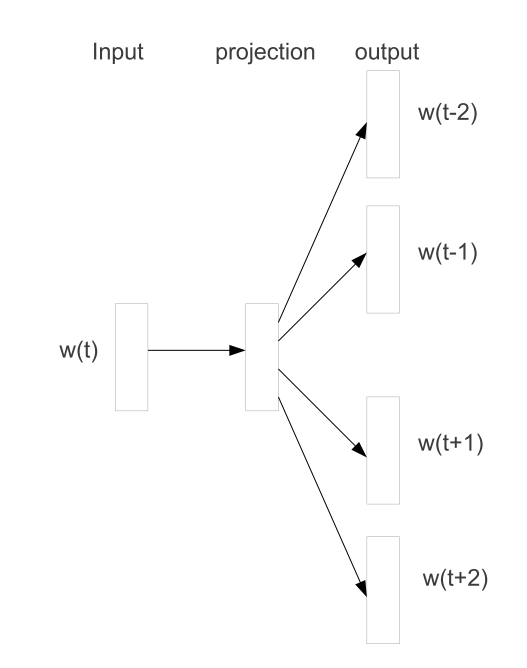
\includegraphics[width=0.5\linewidth, height=0.2\textheight]{fig/cp5/skip-gram-architecture}
%       \caption{The Skip-gram model architecture~\cite{Mikolov2013}}
%       \label{fig:skip-gram}
%   \end{minipage}%
%   \begin{minipage}{0.5\textwidth}
%       \centering
%       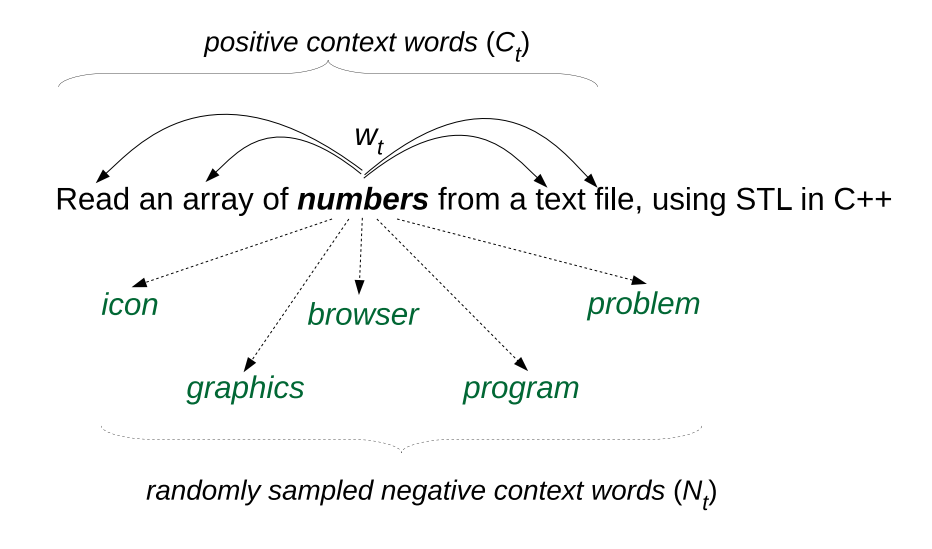
\includegraphics[width=\linewidth, height=0.2\textheight]{fig/cp5/ye-skip-gram-example}
%       \caption{Positive and negative training examples~\cite{Ye2016}}
%       \label{fig:skip-gram-example}
%   \end{minipage}
% \end{figure}



%%%%%%%%%%%%%%%%%%%%%%%%%%%%%%%%%%%%%%%%%%%%%%%%%%%%%%%%%%%%%%%%%%%%%%

\title{Supporting a Developer's Discovery \\ of Task-Relevant Information}
%\subtitle{If you want a subtitle}

\author{Arthur de Sousa Marques}
\previousdegree{B. Computer Science, Universidade Federal de Campina Grande, 2013}
\previousdegree{M. Computer Science,  Universidade Federal de Campina Grande, 2014}

% What is this dissertation for?
\degreetitle{Doctor of Philosophy}

\institution{The University of British Columbia}
\campus{Vancouver}

\faculty{The Faculty of Science}
\department{Computer Science}
\submissionmonth{August}
\submissionyear{2022}

% details of your examining committee
\examiningcommittee{Gail C. Murphy}{Supervisor}
\examiningcommittee{Muhammad Abdul-Mageed}{Supervisory Committee Member}
\examiningcommittee{Reid Holmes}{Supervisory Committee Member}
\examiningcommittee{Magnus Monolith, Other Department}{Additional Examiner} % TODO

% details of your supervisory committee
\supervisorycommittee{Reid Holmes}{Supervisory Committee Member}
\supervisorycommittee{Muhammad Abdul-Mageed}{Supervisory Committee Member}

%% hyperref package provides support for embedding meta-data in .PDF
%% files
\hypersetup{
  pdftitle={ (DRAFT: \today)},
  pdfauthor={Arthur Marques},
  pdfkeywords={Your keywords here}
}

%%%%%%%%%%%%%%%%%%%%%%%%%%%%%%%%%%%%%%%%%%%%%%%%%%%%%%%%%%%%%%%%%%%%%%

\begin{document}

% TODO uncomment
% \maketitle

% \makecommitteepage

% 

\chapter*{Abstract}

The information that a developer seeks to aid in the completion of a task typically exists across different kinds of software artifacts that include substantial natural language text. For instance,
artifacts vary from conversational discussions about bug reports to tutorial descriptions of features in a library.
In the artifacts that a developer consults, only some portions of the text will be useful to a developer's task
and locating such portions can be time-consuming as the artifacts can include substantial text to peruse organized in different ways. For example, it might be easier to locate information
in tutorial artifacts with structured headings whereas artifacts consisting of developer conversations might need to be read in detail. 
% \\

Given the limited time developers have to spend on any task, researchers have 
attempted to aid the developers by proposing a range of techniques to automate the identification of relevant text. 
However, this prior work is generally constrained to one or only a few types of artifacts.  
Enabling a developer access to artifact-specific approaches is difficult to deploy
and support to the multitude of artifact types that is constantly evolving
is challenging, if not impractical.
% \\

In this dissertation, we propose a set of generalizable techniques to aid developers in locating a portion of text that might be useful for a task. These techniques are based on semantic patterns that arise from the empirical analysis of the text relevant to a task in multiple kinds of artifacts, leading us to propose techniques that incorporate the semantics of words and sentences to identify text likely relevant to a developer's task automatically.
We evaluate the proposed techniques assessing the extent to which they identify text that developers deem relevant in different kinds of artifacts associated with Android development tasks. We then investigate how a tool that embeds the most promising semantic-based technique might assist developers while they perform a task. Results show that semantic-based techniques perform equivalently well across multiple artifact types and that a tool that automates the provision of task-relevant text assists developers in effectively completing a software development task.
    


% \cleardoublepage

% %% The following is a directive for TeXShop to indicate the main file
%%!TEX root = diss.tex

%% https://www.grad.ubc.ca/current-students/dissertation-thesis-preparation/preliminary-pages
%% 
%% LAY SUMMARY Effective May 2017, all theses and dissertations must
%% include a lay summary.  The lay or public summary explains the key
%% goals and contributions of the research/scholarly work in terms that
%% can be understood by the general public. It must not exceed 150
%% words in length.

\chapter{Lay Summary}

A software developer usually relies on web pages to find information that helps them complete a software task. 
However, only portions of the text in these web pages might be helpful to the developer's current task.
Finding the relevant parts can be difficult and require much time. The approaches that help developers perform this activity are limited to certain types of web pages, such as community forums, tutorials, and others. 
This thesis explores how we can find information relevant to a developer's tasks in a more general manner. 
First, we study text that developers find relevant to a task. 
Then we propose techniques that find such text automatically. 
We report how a tool built using one of these techniques helps developers perform a task. 
Results show that developers find that the text  identified automatically by the tool has helpful information that assists them in completing a software task.

% \cleardoublepage

% %% The following is a directive for TeXShop to indicate the main file
%%!TEX root = diss.tex

\chapter{Preface}

All of the work presented in this thesis was conducted in the Software Practices
Lab at the University of British Columbia, Point Grey campus.
Parts of the research presented in this dissertation has been previously published in the following articles:


% \begin{small}
\begin{enumerate}
    \item  Arthur Marques, ``\textit{Helping developers search and locate task-relevant information in natural language documents}'', 27th ACM Joint Meeting on European Software Engineering Conference and Symposium on the Foundations of Software Engineering (ESEC/FSE), 2019, pp. 1168-1171, doi: 10.1145/3338906.3341459
    \item  Arthur Marques, Nick C. Bradley and Gail C. Murphy, ``\textit{Characterizing Task-Relevant Information in Natural Language Software Artifacts}'', IEEE International Conference on Software Maintenance and Evolution (ICSME), 2020, pp. 476-487, doi: 10.1109/ICSME46990.2020.00052.
    \item  Arthur Marques, Giovanni Viviani and Gail C. Murphy, ``\textit{Assessing Semantic Frames to Support Program Comprehension Activities}'',  IEEE/ACM 29th International Conference on Program Comprehension (ICPC), 2021, pp. 13-24, doi: 10.1109/ICPC52881.2021.00011.
    \item   Arthur Marques and Gail C. Murphy, ``\textit{Evaluating the Use of Semantics for Identifying Task-relevant Textual Information}'',  2022 IEEE International Conference on Software Analysis, Evolution and Reengineering (SANER), 2022, pp. 240-251, doi: 10.1109/SANER53432.2022.00039
\end{enumerate}
% \end{small}




Part of this work involved other collaborators. Nick C. Bradley contributed in
the interview analysis described in Chapter~\ref{ch:characterizing}.
Alison Li, Katharine Kerr, and Tarc{\'i}sio Teixeira helped 
in the creation of the dataset presented in Chapter~\ref{ch:android-corpus}.
Giovanni Viviani helped in the analysis, design and implementation of the 
semantic parser used in Chapter~\ref{ch:identifying}.
Shaunak Tulshibagwale helped implementing some of the 
data gathering scripts for the 
corpora presented in Chapters~\ref{ch:identifying} and~\ref{ch:assisting}, respectively.
The scripts that gathered data from Stack Overflow are an extension of 
 Nadi and Treude's scripts~\cite{nadi2019Rep}.
Muhammad Abdul-Mageed was a supervisory committee member and helped providing access to the 
Compute Canada research grid used in the design and evaluation of the
approaches described in  Chapter~\ref{ch:identifying}.
Gail C. Murphy was the supervisory author on this project
and was involved throughout the project in concept formation, data analysis, and
manuscript composition.




All projects and associated methods were approved by the University of British Columbia's Research
Ethics Board [certificates \#H18-02104 and \#H19-04054].



% \cleardoublepage

% \tableofcontents
% \cleardoublepage	% required by tocloft package

% \listoftables
% \cleardoublepage	% required by tocloft package

% \listoffigures
% \cleardoublepage	% required by tocloft package

%% The following is a directive for TeXShop to indicate the main file
%%!TEX root = diss.tex

\chapter{Glossary}

This glossary uses the handy \latexpackage{acroynym} package to automatically
maintain the glossary.  It uses the package's \texttt{printonlyused}
option to include only those acronyms explicitly referenced in the
\LaTeX\ source.  To change how the acronyms are rendered, change the
\verb+\acsfont+ definition in \verb+diss.tex+.

% use \acrodef to define an acronym, but no listing
\acrodef{UI}{user interface}
\acrodef{UBC}{University of British Columbia}

% The acronym environment will typeset only those acronyms that were
% *actually used* in the course of the document
\begin{acronym}[ANOVA]
\acro{ANOVA}[ANOVA]{Analysis of Variance\acroextra{, a set of
  statistical techniques to identify sources of variability between groups}}
\acro{API}{application programming interface}
\acro{CTAN}{\acroextra{The }Common \TeX\ Archive Network}
\acro{DOI}{Document Object Identifier\acroextra{ (see
    \url{http://doi.org})}}
\acro{GPS}[GPS]{Graduate and Postdoctoral Studies}
\acro{PDF}{Portable Document Format}
\acro{RCS}[RCS]{Revision control system\acroextra{, a software
    tool for tracking changes to a set of files}}
\acro{TLX}[TLX]{Task Load Index\acroextra{, an instrument for gauging
  the subjective mental workload experienced by a human in performing
  a task}}
\acro{UML}{Unified Modelling Language\acroextra{, a visual language
    for modelling the structure of software artefacts}}
\acro{URL}{Unique Resource Locator\acroextra{, used to describe a
    means for obtaining some resource on the world wide web}}
\acro{W3C}[W3C]{\acroextra{the }World Wide Web Consortium\acroextra{,
    the standards body for web technologies}}
\acro{XML}{Extensible Markup Language}
\end{acronym}

% You can also use \newacro{}{} to only define acronyms
% but without explictly creating a glossary
% 
% \newacro{ANOVA}[ANOVA]{Analysis of Variance\acroextra{, a set of
%   statistical techniques to identify sources of variability between groups.}}
% \newacro{API}[API]{application programming interface}
% \newacro{GOMS}[GOMS]{Goals, Operators, Methods, and Selection\acroextra{,
%   a framework for usability analysis.}}
% \newacro{TLX}[TLX]{Task Load Index\acroextra{, an instrument for gauging
%   the subjective mental workload experienced by a human in performing
%   a task.}}
% \newacro{UI}[UI]{user interface}
% \newacro{UML}[UML]{Unified Modelling Language}
% \newacro{W3C}[W3C]{World Wide Web Consortium}
% \newacro{XML}[XML]{Extensible Markup Language}
	% always input, since other macros may rely on it

% \textspacing		% begin one-half or double spacing

% %% The following is a directive for TeXShop to indicate the main file
%%!TEX root = diss.tex

\chapter{Acknowledgments}



I cannot express how much I am grateful for my supervisor, Gail Murphy. I feel incredibly privileged to have been supervised by someone so respectful, attentive, and inspiring. Thank you. 

I am equally grateful for all the support my family and my partner, Lisley Siqueira, provided me over the last six years. Moving to an entirely new country and starting our life together was a rollercoaster, yet it was a journey full of love, empathy and self-discovery. 

I am thankful to my supervisory committee, Reid Holmes and Muhammad Abdul-Mageed, for all their support and feedback over the last years. Their curiosity encouraged me to explore and learn many new things. I am also thankful to the members of my examining committee, Luanne Sinnamon, Alexander Summers, and Christina von Flach, for their time and effort in reading my thesis and providing insightful feedback. 

I am indebted to many of the friends and colleagues I made at the University of British Columbia, the Software Practices Lab, the Library Research Commons, the Oakridge Adventist Church, and the Vancouver DnD Collective. Many thanks to old-time friends who kept in touch despite being spread across the globe. I cannot name all of you, but I want to thank you all.


Thanks to all the Computer Science Department staff and Elise Vredenbregt for helping with hectic calendars. I would also like to acknowledge the Natural Sciences and Engineering Research Council of Canada for supporting this work. 


\begin{flushright}
Arthur Marques

October 2022
\end{flushright}


\clearpage

\thispagestyle{empty}
\vspace*{\fill}
\begin{flushright}
\emph{To my partner, Lisley Siqueira}
\end{flushright}
\vspace*{\fill}




\clearpage
\thispagestyle{empty}
\vspace*{\fill}

\begin{flushright}
    \emph{Hoje longe, muitas l\'egua}

    \emph{Numa triste solid\~ao}

    \emph{Espero a chuva cair de novo}

    \emph{Pra mim vortar' pro meu sert\~ao}

    --- Asa Branca, song by Luiz Gonzaga
\end{flushright}
\vspace*{\fill}

\clearpage

%%%%%%%%%%%%%%%%%%%%%%%%%%%%%%%%%%%%%%%%%%%%%%%%%%%%%%%%%%%%%%%%%%%%%%

% Body of Thesis (not all sections may apply)
\mainmatter

\acresetall	% reset all acronyms used so far

\setcounter{chapter}{0}
\setcounter{rq}{1}


\chapter{Introduction}
\label{ch:introduction}


\textbf{Thesis statement:} \textit{
    A developer can more effectively complete a software development task when provided
    with text extracted from natural language software artifacts that 
    automatic techniques determine as relevant to the developer's task 
    according to the meaning, or semantics, of the text.    
}



\clearpage



\setcounter{chapter}{1}


\chapter{Related Work}
\label{ch:related-work}



Information foraging~\cite{Pirolli1999}, or the process through which an individual 
obtains knowledge that assists them accomplish a task often experiences paradigm shifts. 
At times, 
an information need was directed to a library clerk 
who would direct an individual towards 
sections of the library with books pertinent to the question 
posed by a person~\cite{saracevic1975}.
Then, when the \acf{web}~\cite{berners1994web} became popular,
individuals started to rely on search engines 
to seek information~\cite{Page1999} now digitally stored in the form of web pages.
Searching for pertinent artifacts, be them books or web pages, 
is one of the first steps to address an information need,
which we detail in Section~\ref{cp2:searching}.


Then, in possession of a pertinent artifact, careful 
inspection of its content might lead a person 
to find the information that they sought. 
However, due to some of the challenges
associated with finding pertinent information within 
an artifact discussed in the previous chapter, researchers from several 
disciplines have considered means to help 
in this activity. 
In Section~\ref{cp2:general-approaches}, 
we detail approaches from related work
that have investigated how to automatically identify relevant text. 
Then, in Section~\ref{cp2:task-approaches}, 
we hone in approaches 
for automating the identification of text 
likely relevant to a software task.




% Most of the techniques that extract information from natural language software artifacts
% are examples of applications that help developers in performing 
% software development activities~\cite{Meyer2017}. 
Given how 
natural language artifacts have become intrinsically
tied to software development~\cite{umarji2008archetypal},
we conclude this chapter with an overview of 
other applications that make use of textual data
to help developers
across many of the tasks in their daily work (Section~\ref{cp2:dev-productivity}).
\art{v4.0}


% In the last chapter, we introduced some of the challenges
% associated with finding
% information relevant to a developer's task.
% In this chapter, we provide background information on 
% a number of empirical studies that give insight into
% the data available in natural language software artifacts 
% and we also present 
% automated tools that extract text from these artifacts.
% In Section~\ref{cp2:text-in-se}, we begin by providing an  
% overview of the types of textual analysis in the literature
% then, in Sections~\ref{cp2:general-approaches}
% and~\ref{cp2:task-approaches}, we
% detail general textual approaches 
% and task-specific approaches
% that identify and extract text from natural language software artifacts, respectively.
% First, we provide an overview on the kinds of approaches 
% used to extract data from natural language software artifacts.
% Then, we detail how these approaches 
% have been used for automating the identification of text 
% likely relevant to a software task~\cite{a}.







\section{Finding Pertinent Artifacts}
\label{cp2:searching}


We start by considering how an individual finds 
artifacts, or documents, which might 
address an information need. 
For this, information foraging theory~\cite{Pirolli1999} explains how a person navigates through  
a search space looking for information patches  based on 
a set of cues about the effort and gains that a patch provides to them~\cite{Pirolli1999}.
A patch can represent both search results or the content within an artifact
and \textit{explicit} or \textit{implicit} factors affect judging the relevance 
of an information patch~\cite{saracevic1975}.
For example,
consider an electronic library catalog and a search for `\textit{android notifications}'.
Figure~\ref{fig:library-catalogue} shows two hypothetical results for this search
to help ilustrate explicit and implicit factors.
An explicit factor might represent how the keywords in the `\textit{subject and genre}' 
directly match one of the keywords used in the query. An implicit factor might represent 
a person's background or previous knowledge, such as how 
the person performing this search 
might know that the first book targets a more general population and 
that it might not be helpful for a software developer.





\vspace{3mm}
\begin{figure}[H]
\noindent\fbox{%
\parbox{\textwidth}{%
{\ttfamily% 
    \begin{scriptsize}
        \begin{enumerate}[itemindent=-1em,leftmargin=1em]
            \item \textbf{Android for Dummies} 

            Author: Gookin, Dan 

            Location: Britannia Branch Library 

            LC Call No.: 004.167 A57G6ad 

            Subject and genre: Android (electronic resource), Smartphone, Mobile computing

            % Synopsis: This book will tell you pretty much everything you need to know about your Android smartphone or tablet in an equally friendly manner, because that's the best way to learn how to get the most from your Android

        \end{enumerate}          
    \end{scriptsize}
    }%
}}
\noindent\fbox{%
\parbox{\textwidth}{%
{\ttfamily% 
    \begin{scriptsize}
        \begin{enumerate}[itemindent=-1em,leftmargin=1em]\setcounter{enumi}{1}
            \item \textbf{Learning Android} 

            Author: Gargenta, Marko 

            Location: Champlain Heights Branch Library 

            LC Call No.: 005.44 A5G2L1 

            Subject and genre: Android (electronic resource), Application software (development), Mobile computing

            % Synopsis: Presents an introduction on the fundamentals of Android to create a variety of applications.

        \end{enumerate}
    \end{scriptsize}
    }%
}}
\caption{Sample library catalog with two results associated with the keyword `android' }
\label{fig:library-catalogue}
\end{figure}




A similar search could be performed on a web search engine\footnote{e.g., \href{https://www.google.com/}{Google} or \href{https://www.bing.com/}{Microsoft Bing}}
and for both library catalogs or web searches, researchers have investigated 
what affects how a person finds pertinent results and their decision to inspect them.
For example, in electronic library catalogs,
Hildreth observed how keyword searches were used more than any other type of searches (e.g., by author or by title)~\cite{hildreth1997}
while other 
others studies observed impatience and near-random search habits in novice librarians~\cite{novotny2004don}.
In contemporary web search engines, researchers have  also 
investigated how individuals formulate queries~\cite{gross2005have, bendersky2012},
how prior knowledge helps them
to more efficiently perform searches~\cite{DeGraaf2014},
and what search results they inspect, going to the lengths
of using eye-tracking technology for this purpose~\cite{Cutrell2007, marcos2015}.



With the prominence of web search engines, other search problems also gained attention.
For example,  Carbonell and Goldstein pioneered the need 
to investigate both the relevance and novelty of search results~\cite{Carbonell1998}.
That is, on one hand, if one returns only relevant resources, it may be the case that all results contain redundant information 
which might leave some information needs unanswered. 
On the other hand, if the search results are too diverse, it might be difficult for an individual 
to find information that corroborates and consolidates some conclusion~\cite{clark2013relevance}.  
This has led researchers to investigated 
how to balance the relevance and novelty of the results retrieved
by a web search~\cite{najork2001, rafiei2010, vieira2011}
and commercial search engines have since considered how to strike a balance
between relevance and novelty.





Across these general studies, and also in software engineering-specific studies~\cite{Starke2009, Brandt2009a, DeGraaf2014},
a common trend is that the identification of good search terms is as, or even more
important than the search algorithm itself~\cite{Kevic2014}. 
Nonetheless, identifying good search terms is often challenging~\cite{novotny2004don, Haiduc2013} and 
as a consequence, many searches are unsuccessful or retrieve resources that 
a person loses time inspecting only to find that they are not pertinent to the task at hand.
This indicates that individuals usually inspect multiple types of artifacts 
before finding relevant information, further motivating
the work presented in this thesis.



% which contrasted how more experienced users were able to better translate an information 
% need into keyword searches that retrieved useful results









\section{Automated Textual Approaches}
\label{cp2:general-approaches}


This section provides a general overview of 
background information on automated textual approaches
applied to natural language software artifacts. 




\subsection{Pattern Matching Approaches}
\label{cp2:pattern-matching}


Regularities in the terms and in the syntactic structure of the 
might be automatically identified via pattern matching.
Pattern matching approaches use regular expressions describing a sequence of tokens that represent
the text to be identified~\cite{Bavota2016}. 
We describe two tools, Krec~\cite{Robillard2015}  and DeMIBuD~\cite{Chaparro2017}, that
illustrate how software engineering 
researchers use pattern matching in conjunction with the lexical or linguistic elements 
in the text to automatically identify 
text useful to certain software development activities.
    


Knowledge Recommender (Krec)~\cite{Robillard2015} 
is an example of a
 tool that uses lexical patterns to 
 automatically detect relevant text in  API documentation. 
Krec's premise is that relevant sentences contain a code element, such as a method or class signature.
These code elements are identifiable via regular expressions 
and Krec contains a catalog of 361 unique patterns 
that identify threats and directives on how to use some API element.
For example, Krec uses the pattern {\small \textit{$\{$may}, \textit{efficient}, \textit{code element regex$\}$}} 
to identify sentences giving instructions about an efficient way to 
perform some operation. 



{\small DeMIBuD} is a linguistic-based approach that 
automatically detect sentences discussing steps to reproduce 
a bug or the bug's expected behaviour~\cite{Chaparro2017}.
It uses a set of 154 discourse patterns
derived from nearly 3,000 bug reports 
to identify such sentences. 
For example, the pattern 
{\small \textit{$\{$subject}, \textit{should/shall (not)}, \textit{complement$\}$}}
captures common ways with which developers describe a system's expected behaviour
and empirical assessment of the patterns used by the tool has shown that it 
detects sentences of interest in bug reports with high accuracy.






Although the heuristics and regular expressions used in these and other studies~\cite{nadi2020, Maalej2013}
are lightweight and effective~\cite{Bavota2016}, 
pattern-matching approaches 
are often specific to certain kinds of domains and types of artifact~\cite{fucci2019}, 
limiting their use in the design of a generalizable technique.







\subsection{Machine Learning Approaches}
\label{cp2:machine-learning}


Regularities in the text or in an artifact's meta-data can also be 
engineered into features that \acf{ML} 
approaches can leverage to automatically identify and classify
text useful to certain software development activities. 



Researchers pose the problem of identifying text 
in a natural language artifact 
as a binary classification problem. 
That is, the use of a number of features 
to predict whether the text is (or not)
relevant to some context~\cite{aa}.
In software engineering, 
binary classifiers have been used for,
for example, classify text that describes steps to reproduce a bug~\cite{Chaparro2016} or 
classify text that explains a certain API element, as when 
Petrosyan et al. used 
 sentence-level features
and meta-data features in a classifier 
that 
identifies explanations about an API element  in a web tutorial~\cite{Petrosyan2015}.




Other classification problems predict which class, out of many, some input text belongs to. 
This type of classification, referred to as multinomial or multi-class classification, 
is of particular interest if 
we consider the taxonomies described in Section~\ref{cp2:text-in-se}.
For example, Arya et al. identified 16 categories of  information available
in open source GitHub issues (e.g., workarounds, solution discussion, task progress, etc.)~\cite{Arya2019}
and they proposed a multinomial classifier 
to automatically identify such categories.








Although valuable, these classifiers are instances of supervised learning methods.
They require training data so that a classifier predicts the correct outcome 
and the cost and effort of hiring skilled workers to produce 
the labeled data for these and other supervised learning approaches
has been a major limitation to their usage in software engineering research~\cite{Arpteg2018, ferreira2021}. As an alternative,
researchers have also explored 
 unsupervised learning methods---\acs{ML} techniques that do not required training data---for the automatic 
identification or classification of the text in natural language artifacts~\cite{aa}.





A common application of unsupervised learning in software engineering
considers the automatic generation of text summaries.
Most often, automatic summaries are produced 
using extractive techniques that select a subset of 
the sentences of an artifact that will compose the summary~\cite{a}.
Among other natural language artifacts,
extractive summarization techniques
have been applied to Stack Overflow posts~\cite{a}, coding tutorials~\cite{a},
or bug reports, as
when Lotufo et al. 
considered the kinds of sentences a developer would find relevant 
to understand a bug report when pressed with time~\cite{Lotufo2012},
and proposed an unsupervised summarization approach 
based on the PageRank algorithm~\cite{Page1999}
to identify these sentences. 




A second set of unsupervised methods focus on clustering data.
These techniques identify 
subsets in the data that have similar properties or features 
and techniques such as \acf{LDA}~\cite{blei2003latent}  have been used both to 
bootstrap the categorization of information in 
natural language artifacts and as part of tools that identify 
portions of the text in an artifact that are helpful to some context. 
As an example of the former, 
 Allamanis and Sutton
applied \acs{LDA}
to gain insight into the types of questions 
asked on Stack Overflow~\cite{Allamanis2013}.
For the latter, tools such as FRAPT
use \acs{LDA} to identity topics in a web tutorial
and then extract sentences explaining API elements from each of the topics identified~\cite{Jiang2017}.


Despite the significant contributions of these and other studies,
one substantial challenge inherent to the supervised and 
unsupervised \acs{ML} approaches 
is that researchers must engineer which 
features their \acs{ML} technique will use~\cite{ferreira2021}.
Hence, \acs{ML} approaches have limitations similar to the pattern 
matching approaches when we consider 
the specificity and cost of engineering such features
for a variety of kinds of artifacts.






\subsection{Deep Learning Approaches}
\label{cp2:deep-learning}





In contrast to the human-engineered features,
\acf{DL} approaches allow the automatic extraction of features 
from training data through a set of mathematical transformations~\cite{Deng2018, zhang2021deep}.
This makes 
deep learning an interesting 
approach to
uncover regularities 
that might not obvious or easily identified
by software engineering researchers,
thus allowing \acs{DL}
to automate the identification of text in natural language software artifacts
with these `hidden' properties. 




Given the wide range of studies that both propose \acs{DL} models~\cite{aa} and that use 
these models for a certain purpose (e.g., machine translation~\cite{lopez2008translation}), 
we focus
on \acs{DL} applications in the 
software engineering domain~\cite{ferreira2021, li2018deep, watson2022}.
First, we discuss neural embeddings and then we present 
neural network models 
for the same range of problems discussed in the machine learning approaches (Section~\ref{cp2:machine-learning}).






A common application of \acs{DL} in software engineering is the usage of neural, or word, embeddings~\cite{Mikolov2013}
for information retrieval purposes. 
Neural, or word, embeddings produce vector representations in a continuous space,
where words with similar meanings are typically close in the vector space model~\cite{harris1954distributional, mikolov2013efficient}. 
Researchers have found that word
embeddings mitigate lexical mismatches in the text found across different 
natural language software artifacts,
using them as a way to compare the semantic similarity of the text~\cite{mihalcea2006}.
Guided by the recent success of word embeddings 
for a variety of software development 
activities, as shown by Ye et al.'s evaluation of word embeddings
for bug localization~\cite{Ye2016}
or Huang and colleagues' study on 
the usage of word embeddings for API recommendation~\cite{Huang2018},
Chapter~\ref{ch:identifying} 
describes how we incorporate word embeddings in the 
design of techniques that automate the identification of task-relevant text. 






Many other \acs{DL} studies in software engineering~\cite{ferreira2021,li2018deep, watson2022}
use neural network architectures 
in binary or multinomial classifiers as well as in extractive text summarization.
For example, Li et al. used an auto-encoder~\cite{liou2014autoencoder}
to produced more accurate and diverse summaries 
for bug reports~\cite{li2018deep} while 
Fucci et al. used a 
recurrent neural network (\acs{RNN}) with 
\acf{LSTM}~\cite{hochreiter1997lstm}
to identify the types of information available in 
API documentation~\cite{fucci2019}.


While \acs{LSTM}s and other \acs{DL} architectures 
handle dependencies between the words of a sentence, 
state-of-the-art architectures such as \acf{BERT}~\cite{Devlin2018Bert}
can also handle dependencies between sentences
and Ara{\'u}jo et al. used \acs{BERT} in sentence pairs 
representing system requirements and user reviews 
to automatically extract requirements from 
mobile application reviews~\cite{Araujo2021}.
We consider that 
establishing relationships 
between sentence pairs is 
a potential way to determine 
sentences from a natural language artifact 
that are relevant to some input task 
and Chapter~\ref{ch:identifying}
further describes how 
we use \acs{BERT} for this goal.



% \section{Automatic Approaches for Identifying Text in Natural Language Software Artifacts}
\label{cp2:text-approaches}



Information useful to a software task can be buried in irrelevant text or attached to 
non-intuitive blocks of text, making it difficult to discover~\cite{Robillard2015}.
Researchers have long recognized the value of assisting developers in 
identifying information of relevance in this natural language
text.
In this section, we detail tools and approaches from related work.




\subsection{Pattern Matching Approaches}
\label{cp2:pattern-matching}


Pattern matching approaches rely on regular expressions describing a sequence of tokens that represent
 a relevant text fragment~\cite{Bavota2016}. Tokens can either represent words or linguistic elements 
extracted using \acf{NLP}.
    
    
As examples  of pattern matching approaches,  {\small DeMIBuD}~\cite{Chaparro2017}
 and Knowledge Recommender (Krec)~\cite{Maalej2013, Robillard2015} are tools that detect relevant sentences in bug reports and API documentation, respectively. 
These tools derive a set of patterns from annotated data and use them as part of heuristics 
that identify relevant text. Krec assumes that any relevant sentence mentions a 
code element (e.g., a class or method name) and it uses  361 unique patterns
to 
detect relevant sentences in API documentation~\cite{Robillard2015}.
In a similar manner, {\small DeMIBuD} uses a set of 154 discourse patterns to detect sentences 
relevant to understanding a bugs observed or expected behaviour and steps to reproduce it,
which are essential to bug triaging tasks.




In Stack Overflow posts,
Nadi and Treude~\cite{nadi2020} have both applied the original set of patterns from Krec~\cite{Robillard2015} 
and proposed heuristics that rely on the conditionality of the text
to identify sentences that help a developer 
decide whether they want to carefully inspect a Stack Overflow posts or skip over it. 



Although the heuristics and regular expressions used in the aforementioned studies 
are often light-weight and effective~\cite{Bavota2016, Maalej2013}, 
pattern matching approaches are often specific to one kind of domain and 
type of artifact~\cite{fucci2019}. 





\subsection{Summarization Approaches}
\label{cp2:summarization}



Extractive text summarization techniques are used in natural language artifacts in software engineering to
produce a summary of the artifact's content. These summaries aim to represent key information that may help a developer complete their task~\cite{Bavota2016}.
There are summarization techniques based on both supervised and unsupervised learning~\cite{moreno2017}
and one can summarize the entire content of an artifact
or content specific input query, as in query-based summarization~\cite{Huang2018, Goldsteinet1999}.




A number of summarization approaches target bug reports and GitHub issues, largely
focusing on key information within these artifacts. 
Rastkar and colleagues~\cite{Rastkar2010} use a supervised learning approach to summarize the content 
of bug reports showing that conversational features used to summarize emails~\cite{Murray2008}
can also be applied to bug reports while
Lotufo et al.~\cite{Lotufo2012} proposed an unsupervised summarization approach 
that automates the identification of sentences that a developer would first read when
a inspecting bug report.



While many of the approaches described above
largely rely on  lexical aspects in text, researchers have also made use
of structured textual information in the artifacts~\cite{Ponzanelli2015, Treude2016, chen2016}. 
For example, Ponzanelli et al. 
proposed a summarization technique that mixes natural language text and structured data 
available on Stack Overflow
to produce more accurate summaries for Stack Overflow answers~\cite{Ponzanelli2015}. 
As another example, DeepSum~\cite{Li2018} pre-processes a bug report dividing sentences 
containing software elements, the reporter of the bug, and any other sentences 
in the bug report to produce summaries containing more diverse information.




A smaller number of summarization approaches have focused
producing task specific summaries.
These approaches pose the problem of finding task-relevant text 
as a query-based extractive summarization problem and
tools such as AnswerBot~\cite{Xu2017}
identify relevant text in Stack Overflow posts 
based on 
the content of the text, how similar that content is with regards to a input query (i.e., task)
and the structured data available on each of the answers in a Stack Overflow post 
(i.e., number of votes or whether an answer is the accepted answer).
Chapter~\ref{ch:identifying}
compares AnswerBot to the techniques that we explore in this thesis.



\subsection{Machine Learning Approaches}
\label{cp2:machine-learning}


\acf{ML} approaches take the text of a natural language software artifact and identify 
the sentences likely relevant to a particular software task using \textit{unsupervised} or 
\textit{supervised learning} methods~\cite{zhang2005machine}.



Supervised learning approaches use a set of features and labeled data
 to train classifiers with the goal of identifying sentences relevant to 
 certain software activity.
We have already presented supervised approaches that use text summarization (\textit{i.e.,}~\cite{Rastkar2010})
and there are also approaches that identify relevant 
parts of software tutorials~\cite{Jiang2016b}
or API documents~\cite{fucci2019, Maalej2013}
and despite their value, 
the cost and effort of hiring skilled workers to produce 
labeled data in software engineering artifacts 
has been a major limitation 
to the usage of supervised learning 
methods in software engineering~\cite{aa}.





Unsupervised learning approaches do not require labelled data and determine 
relevant sentences according to properties inferred from the data. 
DeepSum~\cite{Li2018} and Lotufo et al.'s~\cite{Lotufo2012} techniques are examples of 
unsupervised approaches in the scope of text summarization. Other unsupervised approaches 
(\textit{i.e.,} {\small FRAPT}~\cite{Jiang2017} or HoliRank~\cite{Ponzanelli2015, Ponzanelli2017})
are mostly based around variations of the PageRank~\cite{Page1999} or LexRank~\cite{Erkan2004} algorithms. 
These algorithms represent all the text in an artifact as a graph.
Then, they establish relationships (\textit{i.e.,} weighted edges in the graph) 
between different sentences (\textit{i.e.,} nodes in the graph) 
and select the nodes with highest weights as the most relevant ones.
A crucial step in building the graph is in the definition of 
how to establish  relationships between nodes.
Early approaches~\cite{Lotufo2012, Jiang2017} 
use \ac{VSM}~\cite{Salton1975vsm} 
for this purpose while more modern ones~\cite{Huang2018, silva2019}
use different word embeddings~\cite{Mikolov2013, bojanowski2017FastText},
which we detail in Section~\ref{cp2:deep-learning}.
\red{TODO}










\subsection{Deep Learning Approaches}
\label{cp2:deep-learning}



One substantial challenge of standard \acf{ML}
approaches is that researchers must engineer which 
features or properties of the text to use~\cite{ferreira2021}.
For example, Rastkar et al. uses conversational features in 
the text of a bug report to assist in determining which sentences 
to include in the bug summary~\cite{Rastkar2010}
while Petrosyan and colleagues use 
linguistic and structural properties 
in the text of API documents to determine text 
explaining API elements~\cite{Petrosyan2015}
and given the specificity of such features, 
researchers often question the generalizability
of standard \acs{ML} approaches~\cite{Xiao2018, fucci2019}.



In contrast to the human engineered features,
\acf{DL} approaches allow the automatic extraction of features 
from textual data through a series of mathematical transformations~\cite{Deng2018, zhang2021deep}.
Deep learning has lead to groundbreaking advancements in many 
research areas (e.g., machine translation~\cite{lopez2008translation}) 
and, given its wide range of applications, this section
focuses on its usage in natural language text appearing in software engineering artifacts~\cite{ferreira2021, li2018deep, sharafi2015}.



% and an in-depth explanation of the field is beyond 
% our scope. Therefore, we present \acf{DL} 
% concepts honing in on its applications research.



% At some cost~\cite{strubell2020}, a \acs{DL} neural-network 
% can derive which properties of the text 
% most accurately assist in determining the outcome of some classification 
% task 



% \acf{DL}, which walked hand-to-hand with improvements in computational power and the amount of memory available in modern computer architectures~\cite{}.






\acs{DL} approaches are of particular interest 
software engineering researchers 
since they assist in identifying hidden patterns 
in the natural language text available,
what has ushered in advancements in software engineering areas 
including


~\cite{sharafi2015}




~\cite{sharafi2015} 



can gather diverse corpora, neural networks 








At times, software engineering researchers have argued
that general lexicon techniques 
are insufficient to address text appearing in
software engineering artifacts. 
% Arguments on why lexicon-based natural 
% language techniques are not applicable are often based
% on a need for access to the \textit{meaning}, or semantics, 
% of words, phrases or sentences appearing in the text~\cite{jurafsky2014speech}.
% In this section, 
% we present background information on semantics focusing on
% its usage in software engineering research.



% \subsection{Word Semantics}

Word semantic techniques are mostly rooted on the hypothesis
that similar words appear in similar context~\cite{harris1954distributional}.
This hypothesis gave origin to a series of
\textit{distributional semantic models}~\cite{Ye2016} that aim to infer the meaning of words.
% In this section, we present prominent models used by software engineering researchers.



Distributional semantic models have been used by software engineering researchers 
to improve the 
the retrieval of artifacts pertinent to a certain task. 
Early models, such as \acf{LSI}~\cite{deerwester1990LSI}, 
have been used to, for example, recover traceability links between source code and
software documentation~\cite{marcus2003}.  
\acs{LSI} takes a initial word representation (i.e., a term by document matrix) and applies \acf{SVD}~\cite{klema1980SVD}
to reduce the dimensionality of this matrix, what causes 
words with similar meaning have the same final representation.


Other word semantic models have assisted software engineering researchers in clustering semantically similar artifacts~\cite{zhang2014, layman2016}. For that, researchers have mostly used
\acf{LDA}~\cite{blei2003latent}---a model that assumes that words used in a similar context often pertain to the same subject to produce topics clustering sentences or documents containing semantically related words---to
identify common themes in developers' blog posts~\cite{Pagano2011} or to design tools that identify duplicated bug reports~\cite{nguyen2012, Thung2014}.


% ---among its many applications~\cite{zhang2014, layman2016}---


% Marcus and Maletic apply \acs{LSI} to 

% In software engineering, \acs{LSI} has been widely used to assist requirements traceability~\cite{lucia2007, hayes2006, gethers2011}.

Despite their significant contributions, early models created word vector representations
by counting the frequency or co-occurrence of words, what is substantially inefficient for large corpora~\cite{Ye2016}.
This and other challenges have been lifted by advancements in the fields of \acf{ML} and \acf{DL}~\cite{ferreira2021, li2018deep}, which walked hand-to-hand with improvements in computational power and the amount of memory available in modern computer architectures~\cite{sharafi2015}.


\acs{DL} models built with \textit{neural, or word, embeddings}~\cite{Mikolov2013} 
are of particular interest to this thesis. 
Neural embeddings produce vector representations in a continuous space 
and researchers have shown that they 





% 



\section{Textual Analysis in Natural Language Software Artifacts}
\label{cp2:text-in-se}



In this section, we detail empirical studies investigating 
textual data in natural language software artifacts. 
Such textual data is  rich in semantic information~\cite{dekhtyar2004} 
and we provide and overview of seminal work 
investigating lexical, syntactic, and semantic aspects of the text.




Initial insights about the text of a natural language artifact might be learned focusing on 
the characters or tokens in the text.
This lexical analysis~\cite{jurafsky2014speech} might be used to identify common or unique words 
used in a set of artifacts as well as to identify words that often appear together in the text.
In software engineering research, Bacchelli et al. used lexical analysis to study how developers describe class elements
in nearly 80,000 emails of an Open Source System~\cite{bacchelli2009}.
Their analysis suggests that lexical terms could be 
used as a mean of automatically linking information in development emails to 
the project's source code.







Syntactic analysis concerns the  elements in the text 
and the grammatical relationships between them~\cite{jurafsky2014speech}. 
Part-of-speech tagging and dependency parsing are common applications of syntactic analysis,
where they identify the nouns, verbs, pronouns, and other elements in the text 
and how these elements relate, respectively. 
As an example of a syntactic analysis study in natural language software artifacts, 
Ko and colleagues identified regularities in the syntactic structure of the text 
of nearly 200,000 bug report titles~\cite{Ko2006}, suggesting that these 
regularities could be used for the automatic identification 
of information in bug reports. 






Sentences with similar terms or similar syntactic structure might convey different information
and researchers have also investigated the meaning of the text in natural language software artifacts. 
These studies consider the semantic analysis of the text and 
software engineering researchers have proposed \textit{taxonomies} to explain the type of information 
available in certain kinds of natural language artifacts~\cite{Maalej2013, Arya2019}. 
For example, Di Sorbo et al. have found that 
text in development mailing lists can be classified according to the developers' intentions (e.g., feature request, solution proposal, etc.)~\cite{Sorbo2015},
suggesting that one can automate this classification to assist developers in finding 
certain types of information.
% Other examples include Maalej and Robillard's taxonomy of patterns of knowledge in API documentation
% or Arya et al. analysis of information types in Open Source issues~\cite{Arya2019}.




Most of the textual analysis in related literature reveal similar trends, i.e., 
that there are regularities in the natural language text and that it might be possible 
to automatically identify such text. Nonetheless, 
existing studies focus on the text of a specific 
type of artifact and investigating if whether these regularities 
apply to different kinds of artifacts is still an open question. 
As a first step to investigate this question, 
Chapter~\ref{ch:characterizing}
presents an empirical study that investigates 
the text that developers 
deemed relevant to a software task 
in different kinds of artifact.





%  For example, Figure~\ref{fig:syntactic-analysis} shows the
%  Stanford CoreNLP~\cite{CoreNLP} syntactic analysis for a sentence 
%  about the file system:  `\textit{you can use io.StringIO}'.



% \medskip
% \begin{figure}[h!]
%     \centering
%     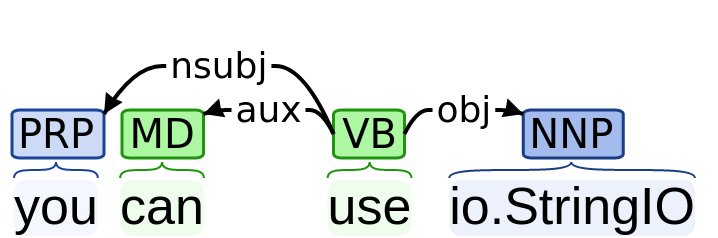
\includegraphics[width=0.40\textwidth]{cp2/textual-analysis.png}
%     \caption{Example of syntactic analysis}
%     \label{fig:syntactic-analysis}
% \end{figure}






% This section details empirical studies analyzing different aspects associated with 
%  natural language software artifacts.






% Early studies on textual analysis in software engineering often focused on program comprehension 
% and the text in the source code~\cite{Woodfield1981, maletic2002},
% but 
% Researchers have long recognized 
% that natural language artifacts 
% are rich in semantic information
% and that 
% better understanding these artifacts
% would lead to improved software~\cite{dekhtyar2004}.






% These studies have helped
% software engineering researchers make more informed decisions 
% on the design of automated tools 
% that identify and extract text from these artifacts---detailed further in this chapter. 




% The empirical analysis provided by these studies 
% has 
% deepened software engineering researchers' knowledge of the type of information available 
% in natural language artifacts 






% Bird at al. used it to investigate social aspects in development mailing lists~\cite{bird2006}. 
% They inspected nearly 102,000 messages on the Apache HTTP Server development lists
%  to find that character editing algorithms~\cite{levenshtein1966}, 
%  helped in unmasking developers' aliases, which helped investigating email 
%  exchange patterns of the key contributors of the project.


% .
% They have sampled 100 emails and identified that text for feature requests 
% often contain expressions in the form of suggestions
% (e.g., `\textit{we should add a new button}'), whereas solution proposals 
% are often expressed in the form of attempts (e.g., `\textit{let's try a new method to compute cost}')





% With regards to meta-data 




% \clearpage


% Several other studies have 
% investigated the meta-data available in
% natural language software artifacts. 
% % In Section~\ref{cp1:example},
% % we have presented an example of meta-data in a Stack Overflow post,
% %  other examples include fields in a bug report~\cite{Davies2014, Breu2010},
% % or tags and labels in GitHub projects~\cite{prana2019}.
% These studies often focus on 
% the frequency with which
% meta-data is available~\cite{Davies2014, bettenburg2008makes, uddin2015},
%  how up-to-date it is~\cite{ahmad2018, dig2006, shi2011}, 
%  and the perils of relying on meta-data for information extraction purposes.
% For example, Zhang et al. has shown that 
% certain comments on Stack Overflow are equally or more informative 
% that the information found in an accepted answer~\cite{zhang2019so}.


% has led software engineering researchers to 
% make more informed decisions on when to use meta-data 
% and how it can assist in the extraction of useful information from natural language 
% artifacts.
% For example, Wang et al. 


% found that 

% the number of votes 
% an answer has on Stack Overflow is 
% equally or more important than 


% ~\cite{wang2018}



% ~\cite{wang2018}









% Findings from these studies led 
% software engineering researchers to discuss the promises and perils of 
% using an artifact's meta-data~\cite{kalliamvakou2014, ahmad2018}.
% For example, an accepted answer on Stack Overflow 
% might not be the correct answer~\cite{wang2018}
% and 
% valuable information exists in elements not
% associated with any meta-data~\cite{zhang2019so},
% which we discussed as part of our 
% scenario about finding information about Android notifications (Section~\ref{cp1:example}).
% 


\section{Techniques for Mining Unstructured Text}
\label{cp2:general-approaches}




In this section, we provide background information on general 
approaches used
by software engineering researchers 
to identify text in natural language software artifacts~\cite{Bavota2016}.
We focus on 
automated approaches that might assist a person in discovering
text that addresses an information need,
presenting both core concepts needed to understand an approach 
and seminal work that has used an approach in 
the context of natural language software artifacts.



% For each approach, we detail 
% present seminal work that has applied 
% these approaches to problems related 
% to software engineering.
% These studies focus on specific tasks such as finding relevant passages in API documentation~\cite{Maalej2013,
% Petrosyan2015, Robillard2015}, learning about API types in code tutorials~\cite{Jiang2016b, Jiang2017},
% or detecting sentences that discuss a bug's expected behaviour~\cite{Chaparro2017}.
% These approaches respectively use the presence of code words, HTML anchor links, or whether a sentence contains
% a modal verb as properties to automatically identify relevant text.




\subsection{Pattern Matching}
\label{cp2:pattern-matching}



Pattern matching approaches use regular expressions describing
a sequence of tokens that represent
the text to be identified~\cite{Bavota2016}. 
We have shown how pattern matching identified
books whose subject contained
the keyword `\textit{android}' (Figure~\ref{fig:library-catalogue})
and the same principle could assist 
in finding parts of an artifact that contain some keyword, 
as many web browsers allow via a `\textit{find in page}' feature (Figure~\ref{fig:find-in-page}).
Nonetheless, this support is very limited and users would have to manually
inspect each match to 
determine if they are relevant or not.






\medskip
\begin{figure}[h!]
    \centering
    
\includegraphics[width=\textwidth]{cp2/find.png}
    \caption{Find in page feature with results for the `\textit{notification}' term}
    \label{fig:find-in-page}
\end{figure}


More automated approaches have also been built using pattern matching, 
as when Panichella et al. 
matched class elements mentioned in development mailing 
 lists to source code files
to assist developers in finding information useful to 
 understanding the source code~\cite{panichella2012}.
Although the heuristics and regular expressions used in this and other studies (e.g.,~\cite{nadi2020, Maalej2013})
are lightweight and effective~\cite{Bavota2016}, 
pattern-matching approaches 
are often specific to certain kinds of domains and types of artifact~\cite{fucci2019}, 
limiting their use in the design of a generalizable technique.


% In development mailing lists, Panichella et al. 
% proposed an automatic approach leveraging \acf{IR} to extract 
% text with useful information that assists in understanding code elements inspected by a developer~\cite{panichella2012}




\subsection{Information Retrieval }
\label{cp2:information-retrieval}


\acf{IR} comprises techniques
or approaches for finding entities (documents, paragraphs, sentences, etc.)
that satisfy an information need~\cite{manning2010IR}.
At its most basic level, 
\acs{IR}
uses the 
frequency or co-occurrence of words (or phrases) to determine the relevance
of an artifact with regards to an information need, often expressed as an input query.


% For that, \acs{IR} identifies and structures all the words, or terms, 
% in an artifact so this information can be used for quick access. 
By counting how frequent  a word is in 
an artifact and across the entire collection of artifacts, 
\acs{IR} can be used to find which artifacts contain that word, or where within an artifact it appears. 
Using this principle, multiple \acs{IR} schemes have been proposed 
to identify text based on 
how not all the words in some vocabulary have the same weight (\textit{TF-IDF})~\cite{luhn1957tf, jones2004idf}, 
how to  represent sentences (\textit{VSM})~\cite{Salton1975vsm}, 
or how to account for different words that appear interchangeably in some context (\textit{LSI})~\cite{dumais1994latent}.



% Information retrieval applications span several disciplines and it has been used 
% to, for example, assist health workers in searching for medical records~\cite{hanauer2015}
% or to help law practitioners in understanding government regulations~\cite{lau2005legal}.

In natural language software artifacts, 
information retrieval has been used 
as part of approaches that
automatically identify sentences  that a developer would first read in a bug report 
when pressed with time~\cite{Lotufo2012},
or in approaches that help cluster software components to aid program comprehension of a software system~\cite{Marcus2003}.
In this dissertation, we combine information retrieval and word embeddings 
to identify relevant text across different kinds of artifacts, as Chapter~\ref{ch:identifying} further details.



\subsection{Natural Language Processing }
\label{cp2:nlp}


\acf{NLP} relies on the lexical or syntactical analysis of the text~\cite{jurafsky2014speech}
and such analyses might assist in the automatic identification of text that satisfies an information need. 
To illustrate some of the elements obtainable using \acs{NLP}, we consider a short sentence 
instructing how to perform a file system operation: ``\textit{you can use io.StringIO}''.
Figure~\ref{fig:nlp-analysis} shows elements extracted for this sentence using two \acs{NLP} techniques,
namely \acf{POS} tagging and dependency parsing.
The former assigns tags  ({\small \textit{PRP}, \textit{VP}, \textit{NNP},} etc.) to each word 
in a sentence~\cite{taylor2003penn} while the latter identifies
relationships between them, such as how 
`\textit{io.StringIO}' is the direct object (\textit{obj})
associated with the verb `\textit{use}'.



\medskip
\begin{figure}[h!]
    \centering
    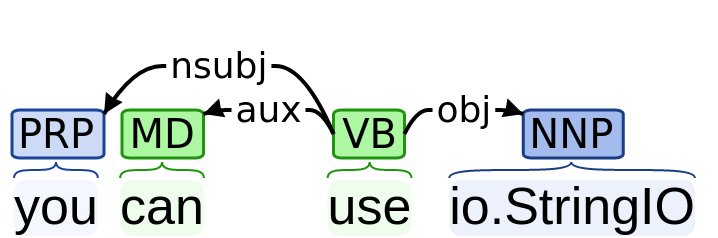
\includegraphics[width=0.40\textwidth]{cp2/textual-analysis.png}
    \caption{Syntactic elements for a sentence giving instructions about how to perform some file system operation}
    \label{fig:nlp-analysis}
\end{figure}


As an example of the application of \ac{NLP} to software engineering text,
Robillard  and Chhetri proposed a tool (Krec)
that uses \acs{POS} tagging to automatically 
identify text with threats and directives on how to use some API element~\cite{Robillard2015}.
As another example, {\small DeMIBuD}
is an automatic approach that uses dependency parsing
to automatically detect sentences discussing a bug's expected behaviour~\cite{Chaparro2017}.
In this work, we use \acs{NLP} as part of our 
analysis of the text deemed relevant to a set of software tasks (Chapter~\ref{ch:characterizing}).



\subsection{Machine Learning }
\label{cp2:machine-learning}



Several other studies have investigated the text 
of various kinds of natural language artifacts and 
the meta-data available on them~\cite{Ko2006, Maalej2013, Arya2019}.
Findings arising from these empirical studies
indicated regularities in the text and meta-data of 
an artifact which could be engineered into 
features that a  \acf{ML} technique could use to automatically identify or classify
text that addresses certain information need~\cite{Bavota2016}. 



Machine learning techniques can be categorized 
according to how they make use of available data. 
Supervised learning approaches use a set of features and labeled data
to train classifiers for detecting entities of interest (e.g., text, images, etc.)
while unsupervised learning approaches do not require labeled data and 
identify entities according to properties inferred from the data.



\subsubsection{Supervised Learning }
\label{cp2:supervised}


With regards to supervised learning approaches, 
we consider the families of classifiers that 
determine
\textit{(1)} if some entity belongs or not to a given class, as in binary classification
\textit{(2)} which class, out of many, some input entity belongs to, as in multinomial classification, or
\textit{(3)} which classes can be assigned to a given input, as in multi-label classification~\cite{alpaydin2020ml},
 and we detail their application to software engineering problems.



% Binary classifiers can be expressed as functions in the form of 
% $f(x) \arrowkeyright y$, where $x$ is a vector of features and $y \in {1, 0}$.
% Hence, it indicates whether $x$ belongs or not a given class.



Among other applications, binary classifiers have been used 
to classify text in bug reports that describes (or not) steps to reproduce a bug~\cite{Chaparro2016}
or  to classify paragraphs which contain explanations 
about API elements in a web tutorials\cite{Petrosyan2015}.
In turn, multinomial classifiers have been mostly used 
to identify a category, out of many, that represents the type of information 
associated with some text. For instance, Arya et al. identified 16 categories of  information available
in open source GitHub issues (e.g., workarounds, solution discussion, task progress, etc.)
and they proposed a multinomial classifier 
to automatically identify such categories~\cite{Arya2019}.
In a similar manner, Fu and colleagues consider 
five types of decisions that might arise during 
email exchanges (e.g., design, testing, management decisions, etc.)
and they proposed a multinomial classifier 
to automatically identify all the decisions present in emails of
a development mailing list~\cite{fu2021}.





Regardless of the type of classifier, these approaches are typically built 
with training data containing human-engineered features and the cost and effort of hiring skilled workers to produce 
the labeled data for these and other supervised learning approaches
has been a major limitation to their usage in software engineering research~\cite{Arpteg2018, ferreira2021}.




\subsubsection{Unsupervised Learning}
\label{cp2:unsupervised}



Common applications of unsupervised learning 
to natural language software artifacts 
comprise text summarization~\cite{Goldsteinet1999} and data clustering, which might help an individual both in understanding the key information in an 
artifact and also in deciding which information patches are 
 worth of their time~\cite{Lotufo2012}.


Unsupervised summarization approaches are often based on 
variations of the PageRank algorithm~\cite{Page1999}, and these approaches identify
the most central sentences in an artifact based on a set of relationships
established between all the sentences in that artifact.
Among other natural language artifacts,
extractive summarization techniques
have been applied to Stack Overflow posts~\cite{Ponzanelli2015},
coding tutorials~\cite{Li2018},
or bug reports, as
when Li et al. summarized 
key elements required to understand a bug and its resolution~\cite{li2018deep}.




A second family of unsupervised techniques focuses on clustering data.
These techniques use properties or features in the data to 
identify 
subsets with similar characteristics. 
Techniques that cluster data, such as \acf{LDA}~\cite{blei2003latent},
have been used by software engineering researchers to both 
bootstrap the categorization of information in 
natural language artifacts and as part of tools that identify topics in the text. 
For instance, Allamanis and Sutton
applied \acs{LDA}
to gain insight into the types of questions 
asked on Stack Overflow~\cite{Allamanis2013}
while FRAPT is a tool that 
uses \acs{LDA} to identity topics in a web tutorial
as well as relevant sentences in each of the topics identified~\cite{Jiang2017}.



Although unsupervised techniques lift the need for labeled training data,
they still use human-engineered features, 
which are often specific to certain 
types of artifact. Therefore, 
both supervised and unsupervised \acs{ML}
have limitations that might prevent their usage 
in the design of a generalizable technique.




\subsection{Deep Learning }
\label{cp2:deep-learning}



In contrast to the human-engineered features,
\acf{DL} approaches allow the automatic extraction of features 
from training data through a set of mathematical transformations~\cite{Deng2018, zhang2021deep}.
This makes 
deep learning an interesting 
approach to
uncover regularities 
that are not obvious or easily identified
by software engineering researchers.



A common application of \acs{DL} in software engineering is the usage of neural, or word, embeddings~\cite{Mikolov2013}
for information retrieval purposes. 
Neural, or word, embeddings produce vector representations in a continuous space,
where words with similar meanings are typically close in the vector space~\cite{harris1954distributional, mikolov2013efficient}. 
Researchers have found that word
embeddings mitigate lexical mismatches in the text found across different 
natural language software artifacts,
as shown by Ye et al.'s evaluation of word embeddings
for bug localization~\cite{Ye2016}
or Huang and colleagues' study on 
the usage of word embeddings for API recommendation~\cite{Huang2018}.
Guided by these findings, Chapter~\ref{ch:identifying} describes 
how we use word embeddings in the identification 
of task-relevant text.



Many other \acs{DL} studies in software engineering~\cite{ferreira2021,li2018deep}
use neural network architectures 
for the same range of problems discussed in Section~\ref{cp2:machine-learning}.
As explained by Watson et al.~\cite{watson2022},
neural network architectures are composed of several layers 
that perform a series of transformations on data passing through them. 
A set of parameters controls these transformations and 
adjust the model being trained so that it can predict 
the right outcome for any given input.
Using these concepts, researchers have proposed 
several  \acs{DL} architectures (e.g., \acs{RNN}s~\cite{rumelhart1986rnn, sutskever2014seq2seq}, encoder-decoders~\cite{bahdanau2014neural}, Transformers~\cite{Vaswani2017attention}, etc.) 
suitable for different problems. 
For instance,
Li et al. used an auto-encoder~\cite{liou2014autoencoder}
to produce more accurate and diverse summaries 
for bug reports~\cite{li2018deep} while 
Fucci et al. used a 
recurrent neural network (\acs{RNN}) 
to identify the types of information available in 
API documentation~\cite{fucci2019}.

% with \acf{LSTM}~\cite{hochreiter1997lstm}


Similar to supervised \acs{ML} approaches, deep learning approaches 
typically require large amounts of data for training purposes.
Nonetheless, recent advancements on the usage of
pre-trained models 
have lifted some of these limitations~\cite{erhan2010pre-train}.
In Chapter~\ref{ch:identifying},
we investigate how we can use a state-of-the-art architecture, namely BERT~\cite{Devlin2018Bert},
to identify relevant text across different types of artifacts.




% \subsection{Summary of Techniques}


% \art{Should I have a summary section and a table bundling examples of studies for each technique and the artifacts that they apply to? }






% Researchers pose the problem of identifying text 
% in a natural language artifact 
% as a binary classification problem. 
% That is, the use of a number of features 
% to predict whether the text is (or not)
% relevant to some context~\cite{aa}.
% In software engineering, 
% binary classifiers have been used for,
% for example, classify text that describes steps to reproduce a bug~\cite{Chaparro2016} or 
% classify text that explains a certain API element, as when 
% Petrosyan et al. used 
%  sentence-level features
% and meta-data features in a classifier 
% that 
% identifies explanations about an API element  in a web tutorial~\cite{Petrosyan2015}.




% Other classification problems predict which class, out of many, some input text belongs to. 
% This type of classification, referred to as multinomial or multi-class classification, 
% is of particular interest if 
% we consider the taxonomies described in Section~\ref{cp2:text-in-se}.
% For example, Arya et al. identified 16 categories of  information available
% in open source GitHub issues (e.g., workarounds, solution discussion, task progress, etc.)~\cite{Arya2019}
% and they proposed a multinomial classifier 
% to automatically identify such categories.








% Although valuable, these classifiers are instances of supervised learning methods.
% They require training data so that a classifier predicts the correct outcome 
% and the cost and effort of hiring skilled workers to produce 
% the labeled data for these and other supervised learning approaches
% has been a major limitation to their usage in software engineering research~\cite{Arpteg2018, ferreira2021}. As an alternative,
% researchers have also explored 
%  unsupervised learning methods---\acs{ML} techniques that do not required training data---for the automatic 
% identification or classification of the text in natural language artifacts~\cite{aa}.





% A common application of unsupervised learning in software engineering
% considers the automatic generation of text summaries.
% Most often, automatic summaries are produced 
% using extractive techniques that select a subset of 
% the sentences of an artifact that will compose the summary~\cite{a}.
% Among other natural language artifacts,
% extractive summarization techniques
% have been applied to Stack Overflow posts~\cite{a}, coding tutorials~\cite{a},
% or bug reports, as
% when Lotufo et al. 
% considered the kinds of sentences a developer would find relevant 
% to understand a bug report when pressed with time~\cite{Lotufo2012},
% and proposed an unsupervised summarization approach 
% based on the PageRank algorithm~\cite{Page1999}
% to identify these sentences. 




% A second set of unsupervised methods focus on clustering data.
% These techniques identify 
% subsets in the data that have similar properties or features 
% and techniques such as \acf{LDA}~\cite{blei2003latent}  have been used both to 
% bootstrap the categorization of information in 
% natural language artifacts and as part of tools that identify 
% portions of the text in an artifact that are helpful to some context. 
% As an example of the former, 
%  Allamanis and Sutton
% applied \acs{LDA}
% to gain insight into the types of questions 
% asked on Stack Overflow~\cite{Allamanis2013}.
% For the latter, tools such as FRAPT
% use \acs{LDA} to identity topics in a web tutorial
% and then extract sentences explaining API elements from each of the topics identified~\cite{Jiang2017}.


% Despite the significant contributions of these and other studies,
% one substantial challenge inherent to the supervised and 
% unsupervised \acs{ML} approaches 
% is that researchers must engineer which 
% features their \acs{ML} technique will use~\cite{ferreira2021}.
% Hence, \acs{ML} approaches have limitations similar to the pattern 
% matching approaches when we consider 
% the specificity and cost of engineering such features
% for a variety of kinds of artifacts.








% pre-trained models that do not require large amounts of training data to our domain problem~\cite{devlin2018bert, Ye2016}. With this approach, we revisit findings on the trade-offs of using machine learning techniques to mine textual data~\cite{Chaparro2017, Bavota2016}.




% using them as a way to compare the semantic similarity of the text~\cite{mihalcea2006}.
% Guided by the recent success of word embeddings 
% for a variety of software development 
% activities,,
% Chapter~\ref{ch:identifying} 
% describes how we incorporate word embeddings in the 
% design of techniques that automate the identification of task-relevant text. 






% ,
% thus allowing \acs{DL}
% to automate the identification of text in natural language software artifacts
% with these `hidden' properties. 









% These studies focus on specific tasks such as finding relevant passages in API documentation~\cite{Maalej2013,
% Petrosyan2015, Robillard2015}, learning about API types in code tutorials~\cite{Jiang2016b, Jiang2017},
% or detecting sentences that discuss a bug's expected behaviour~\cite{Chaparro2017}.
% These approaches respectively use the presence of code words, HTML anchor links, or whether a sentence contains
% a modal verb as properties to automatically identify relevant text.
% Given how quickly developers progress to using new kinds of technology to
% record pertinent information (e.g., slack~\cite{Storey2017, Lin2016}),
% it may be difficult to scale such artifact-centric approaches to cover the range of
% artifacts that could be returned from a search.
% A second issue arises from the fact that coding procedures used to determine relevancy
% in these studies do not consider disagreements~\cite{Stol2015}.
% That is, there are many criteria in how individuals
% assess relevance~\cite{Barry1994, Barry1998, Freund2015}
% and there are no guarantees that
% developers will use the same properties to determine text relevant to their tasks~\cite{Freund2013, Freund2015}.
% In contrast, our study does not pre-assume any relevance cues, and instead,
% we leave the decision of what text is perceived as relevant to a particular task to
% the participants in our experiment.









% Knowledge Recommender ()
% is an example of a
%  tool that uses lexical patterns to 
%  automatically detect relevant text in  API documentation. 
% Krec's premise is that relevant sentences contain a code element, such as a method or class signature.
% These code elements are identifiable via regular expressions 
% and Krec contains a catalog of 361 unique patterns 
% that identify threats and directives on how to use some API element.
% For example, Krec uses the pattern {\small \textit{$\{$may}, \textit{efficient}, \textit{code element regex$\}$}} 
% to identify sentences giving instructions about an efficient way to 
% perform some operation. 



%  is a linguistic-based approach that 

% It uses a set of 154 discourse patterns
% derived from nearly 3,000 bug reports 
% to identify such sentences. 
% For example, the pattern 
% {\small \textit{$\{$subject}, \textit{should/shall (not)}, \textit{complement$\}$}}
% captures common ways with which developers describe a system's expected behaviour
% and empirical assessment of the patterns used by the tool has shown that it 
% detects sentences of interest in bug reports with high accuracy.



% ~\cite{krallinger2017}



% ~\cite{mcdonough2019}
% 



\section{Task-specific Techniques}
\label{cp2:task-approaches}



Although certainly valuable, the techniques mentioned in Section~\ref{cp2:general-approaches}
do not extract text tailored to 
a specific software task. In other words, they identify 
a set of sentences in an input artifact regardless of the developer's task. 
In contrast, this section focuses on task-specific techniques.
% where core component to identifying information specific to a task 
% is a query which represents the task being performed~\cite{Bavota2016}. 
% This query can be explicitly formulated by a developer 
% or implicitly derived from the code or the context 
% in which a developer is working.

%  (as described in Section~\ref{cp2:unsupervised})
A small number of studies~\cite{Xu2017, silva2019, liu2019qapi} 
 formulate the problem of identifying task-specific text 
 in specific types of artifacts as 
a special case of query-based summarization~\cite{Goldsteinet1999}. That is, 
instead of producing a summary for the entire content of 
an artifact,
these studies first use information retrieval techniques
to identify a subset 
of sentences relevant to a task and then, 
a summary of these key sentences is produced.



AnswerBot~\cite{Xu2017} is an example of a query-based summarization tool.
It uses word embeddings to find which sentences in a Stack Overflow answer 
are most similar to a query representing a developer's task.
The tool uses semantic similarity in conjunction with 
Stack Overflow's meta-data to decide which text  it should include
in the summary that it will produce. 
A second query-based summarization tool by Liu et al. parses the content 
of API documents to build a knowledge graph of the information within this type of artifact. 
Their tool, KG-APISumm~\cite{liu2019qapi}, uses this graph 
to find nodes with text that matches the text of an input task, 
producing a task-specific summary for this type of artifact. 


These techniques
target one type of artifact and they also use an artifact's meta-data to 
assist in the automatic identification of task-relevant text, thus
limiting their use across the
many different kinds of artifacts developers encounter
daily in their work. 
For example, AnswerBot uses the number of votes an answer has to decide which text it will use to produce a summary~\cite{Xu2017}
while KG-APISumm uses 
code blocks, HTML anchor links and other properties exclusive to API documents to build the knowledge graph used as part of its summarization approach~\cite{liu2019qapi}.
We differ from these studies 
by not using assumptions 
specific to certain kinds of artifacts
and by considering how to identify task-relevant text 
in a more generalizable manner.





% As a result, these approaches are constrained to specific artifacts and do not 
% generalize to the different kinds of artifacts a developer might consult. 





% the text identified by these techniques might indeed 


% contain information relevant to a specific software task,
% a key component that distinguish the techniques 
%  is that they 




% We now consider applications that assist developers in 
% searching for artifacts that contain information 
% for a particular task
% and that automate the identification 
% of text likely relevant to a developer's task;




% We use the terms change task and task to refer to any change to a software system that serves a predefined purpose, such as a bug fix or an enhancement.


% In this section, we detail textual approaches that automate the identification 
% of text likely relevant to a developer's task. 



% Task-specific automated approaches 
% use many of the techniques discussed in Section~\ref{cp2:general-approaches}
% in conjunction with the text in a developer's task
%  or the code in a developer's workspace
% as potential ways  
% to identify task specific information.
% A seminal tool that exemplifies 
% how these sources assist in locating task specific information is
% Hipikat~\cite{Cubranic2005}.
% It takes a query explicitly prompted by a developer 
% or implicitly based on the code that the developer 
% has inspect and  
% it recommends artifacts from a project's archive 
% that are pertinent to the query.
% While Hipikat makes recommendations at the artifact level,  
% this approach could be fine-tuned to identify 
% parts of an artifact that are relevant~\cite{Cubranic2005}
% and other studies have since built upon this core idea. 
% For example, Deep Intellisense 
% uses pattern matching to 
% identify 
% artifacts containing text that 
% would assist a developer
% better understand the code that they inspect~\cite{Holmes2008}
% while 
% CueMeIn takes the code 
% a developer is currently editing and it
% automatically finds 
% excerpts from web tutorials 
% that might contain explanations 
% for the classes and methods 
% of the method being edited~\cite{sun2021}. 










% In Section~\ref{cp2:general-approaches}, we described 
% techniques for mining textual data. 
% These techniques identify text that might assist a developer 
% in performing certain activities such as finding 
% text describing how to use an API~\cite{Robillard2015} 
% or finding text with decisions made by members of a development 
% community~\cite{fu2021}.
% 



\section{Improving Developers' Productivity}
\label{cp2:dev-productivity}


\art{stopped reviewing related-work here}


% The tools and approaches presented in Sections~\ref{cp2:general-approaches}
% and~\ref{cp2:task-approaches}
% are examples of studies that help developers in locating 
% information that assists them in completing a software task.
% These studies fit in the bigger context 
% of software engineering research 
% facilitating or improving the quality of a developer's work~\cite{Kersten2006, Meyer2017, satterfield2020}. 





% As part of their work, developers engage in many sensemaking and decision-making activities~\cite{sillito2006} and several studies have investigated how to 
% provide means to better  
% assist developers in performing such activities~\cite{Liu2018Unakite, liu2021, barnett2015}.
% For example, 
% Ponzanelli et al. proposed a tool, Libra, that monitors the web pages a developer 
% has navigated and uses that to show 
% how similar or not the results of a new web search are in comparison to the already navigated 
% pages, which offers contextual information-seeking support~\cite{Ponzanelli2017}.



% Researchers have also been interested in 
% making knowledge bases
% that developers working on a task can benefit from. 
% In Section~\ref{cp2:task-approaches} 
% we cited Hipikat~\cite{Cubranic2005}, a seminal tool that exemplifies this concept in action.
% Based on the current code being inspected by a developer or based on a query prompted by a developer, 
% it recommends artifacts from a project's archive 
% that are pertinent to the code being inspected.
% This archive, or project memory, is produced 
% based either on relationships between the artifacts in a software project 
% or based on the source code changed in a bug fix or feature request~\cite{Cubranic2005}.
% Other tools like Strata summarize knowledge produced by developers 
% while they navigate on the web so that other developers
% can use this knowledge to have a 
%  head start when performing similar tasks~\cite{liu2021}.




% We build upon many of the research procedures outlined 
% in these and many other studies in the field. 
% For example, in the evaluation of Strata, 
%  Liu et al. describe procedures 
% considering how a control and tool-assisted group 
% complete information-seeking tasks~\cite{liu2021},
% which assisted in the design of our experiment for 
% evaluating an automated approach to
% task-relevant text identification (Chapter~\ref{ch:assisting}).









\setcounter{chapter}{2}


\chapter{Characterizing Task-relevant Text}
\label{ch:characterizing}



In the last chapter,
we described several studies that analyze text in software engineering artifacts
and many approaches that attempt to automatically extract relevant information from
these natural language artifacts. However, 
we have described that
most of these approaches focus on 
one or only a 
few types of artifacts
leaving open the question of 
how to identify text relevant to a task regardless of an artifact's type.


% To design
% generalizable technique as described in our thesis statement,
% we ask whether
% there is consistency in the text
% that software developers identify as relevant to a task across
% different kinds of artifacts, and if there is consistency, we also ask
% what are common relevance cues in the portions of
% the text identified as relevant?
% Determining common cues that
% developers use regardless of an artifact's type
% could provide valuable
% insights for the design of a generalizable 
% technique~\cite{Bavota2016}.




To address this questions, 
this chapter presents an
\textit{empirical study} in which we
investigate whether 
there are common cues in the text
that software developers identify as relevant to a task across
different kinds of artifacts.
To investigate such cues, we 
asked 20 participants with
software development experience to identify relevant text within
selected artifacts for six distinct software development tasks.
We analyze the text that participants considered relevant 
to gain insight into properties of the text 
that are indicative of its relevance to a task~\cite{das2014frame, jurafsky2014speech}
while also reporting the participants'
reasoning process for determining relevance,
 gathered through interviews
that we use as part of our analysis on
their information-foraging process.



We start by presenting the research questions that guide 
the design of our study (Section~\ref{cp3:method}).
We then detail experimental procedures (Section~\ref{cp3:experiment}) 
and results (Section~\ref{cp3:results}),
concluding the chapter with a summary of our findings (Section~\ref{cp3:summary}).



\section{Motivation}
\label{cp3:method}

% To produce a solution for a task, a developer engages in a variety of information-seeking activities which are the focus of our experiment.
% Particularly, we focus on the text that a developer deems relevant to working on a software task,
% which we define as ``problem reports and feature request descriptions often recorded in an issue tracking system such as Bugzilla''~\cite{Cubranic2005}.


In Chapter~\ref{ch:related-work} we described limitations 
of existing approaches for identifying task-relevant 
text across different types of artifacts. 
To investigate how to relax these limitations, we consider three questions:


\begin{enumerate}[label=\textit{RQ\arabic*},leftmargin=*]

    \item \textit{How much agreement is there between developers about the text
    relevant to a task?} With this question, we seek to understand
    the amount of information sought for task completion
    and whether individuals see the same text as
    relevant to a task.

    \item \textit{What are common cues to the relevancy of text to a task?}
    With this question, we seek to determine if the rules governing how natural language information
    is constructed can guide us to information relevant to a task~\cite{Kintsch1978a}.
    We consider whether there
    are patterns in the  syntactic structure and in meaning of text identified as relevant.

    \item \textit{How do developers determine if text is relevant to a task?}
    With this question, we seek to identify common themes in developers' identification of task-relevant text. For instance, what are common challenges or factors that affect a developers' judgment on the relevancy of the text to a task?

\end{enumerate}



The first research question seeks to characterize text
in documents relevant to a task.
The second research question refers to the text itself.
It analyzes possible syntactic or semantic
predictive cues that may originate from commonalities in any of the text that developers deem relevant to the tasks we present them.
The last research question considers qualitative aspects that might provide
further insights to how developers identify relevant text.



\section{Experiment}
\label{cp3:experiment}



To investigate which text within a natural language artifact software developers deem as relevant to a task,
 we decide for a controlled experiment
 as it allows us to investigate the behavior of multiple developers
over a consistent set of artifacts.



In the experiment, detailed in the following subsections,
we asked 20 participants to highlight portions of a curated
set of artifacts relevant to completing six different development tasks;
 highlighting was followed by post-experiment 
interviews to understand the
strategies that participants employed to identify relevant text,
providing us both 
quantitive data (in the form of the highlights produced) 
and qualitative data (in the form of the interview transcripts) 
which we use to answer the research questions 
presented earlier in this chapter.






\acs{UBC} Behavioural Research Ethics Board  approved this experiment under the certificate \textit{H18-02104}.
The experiment's supplementary material is also publicly available~\cite{cp3_supplementary_material}.




\subsection{Tasks}
\label{cp3:method-tasks}


The six tasks in our experiment provide for a variety of information-seeking activities observed from earlier
studies, which include when a developer
refers to API documentation or Q\&A websites for API usage purposes~\cite{umarji2008archetypal, Singer1998,robillard2011field};
evaluates a possible reusable library to be incorporated into their implementation~\cite{umarji2008archetypal}; or
confirms a system's behaviour referring to past discussions in community forums or in the system's documentation~\cite{umarji2008archetypal, Lotufo2012, Singer1998}.
To design tasks for these activities, we applied criteria described by Petrosyan and colleagues~\cite{Petrosyan2015}, namely that
tasks must encompass common application domains and that the tasks' artifacts must be publicly available.


Table~\ref{tbl:tasks-overview-cp3} outlines the tasks designed.
For each task, the table provides a brief description and the task name, which refers to an identifier pertaining the topic or the system related to the task.
From this point forward, we will refer to the tasks according to these identifiers.
\texttt{Bugzilla} and \texttt{Yargs} are API usage tasks; \texttt{Networking} and \texttt{Databases} ask participants to evaluate and decide upon the adoption of a certain technology or framework; and finally, \texttt{GPMDPU} and \texttt{Lucene} describe scenarios where a participant 
has to understand the system's behaviour. 


Our decision to use a number of different systems employing
a variety of technologies aims to minimize the effects that might result from a participant being
well-acquainted with a particular system or technology~\cite{Wildemuth2012, DeGraaf2014}. 



\begin{table}
\caption{Tasks overview}
\begin{scriptsize}
\vspace{-1mm}  


\begin{threeparttable}    
\rowcolors{2}{}{lightgray}
\begin{tabular}{ll}
\hline    
\textbf{Task} & \textbf{Description} \\ 
\hline
\hline
Bugzilla & 
\parbox[l][0.9cm][c]{11cm}{Locate information about Bugzilla's REST API custom fields and how they can be included as part of the \texttt{GET /rest/bug} payload}  \\
%
Databases & 
\parbox[l][0.9cm][c]{11cm}{Review Q\&A forums and decide between the adoption of ORM or JDBC for a system's database being migrated from C to Java}  \\ 
%
GPMDPU & 
\parbox[l][0.9cm][c]{11cm}{Locate constraints or limitations about the GPMDPU shortcuts feature in order to work in a patch for this feature}  \\
%
Lucene & 
\parbox[l][0.9cm][c]{11cm}{Review the Lucene documentation and bug reports to understand how it computes similarity scores during indexing, particularly the BM25 score function, such that you can address a change request} \\
%
Networking & 
\parbox[l][0.9cm][c]{11cm}{Review the MDN documentation and Q\&A forums to decide between the adoption of Server-sent events or WebSockets technologies for a notification system being developed using Javascript } \\ 
%
Yargs & 
\parbox[l][1.2cm][c]{11cm}{Review the Yargs documentation and bug reports to check whether the API provides support for parsing mutually exclusive arguments, which is a requirement for a command line tool being developed in Python } \\
\hline
\end{tabular}
\end{threeparttable}    
\end{scriptsize}
\smallskip
\label{tbl:tasks-overview-cp3}
\end{table}




\subsection{Artifacts}
\label{cp3:method-artifacts}



For each task, we also needed to choose a set of artifacts for a
participant to peruse for relevant information to the task.  Based on
observations about the most common information sources sought in
development tasks~\cite{Li2013, Ponzanelli2017},
we focused on API documentation, Q\&A websites, and
bug reports.
For each task, a participant should consider on average three artifacts extracted
from one or more information sources.
We describe selection criteria for the artifacts and information sources as follows.


% \footnote{
% e.g.: https://www.google.com/search?q=bugzilla+REST+API
% }

To select the artifacts, for each task, we performed
searches and inspected the top 10 results retrieved by Google search engine, Stack Overflow, and in a
system's bug tracking system to select a set of candidate artifacts that could
assist in task completion.
For some tasks, the list of candidate
artifacts contained a single kind of artifact (e.g., bug
reports). For others, multiple kinds of candidate artifacts applied
(e.g., API documentation and Q\&A websites). 
Due to the varied availability of artifact types per task, 
we ensured that across
the six tasks, each kind of artifact appeared in at least half of the
tasks.



To produce the curated set of artifacts for each task, we then carefully read each candidate artifact.
Selection criteria considered an artifact's content and possible effects that 
could arise from interacting with a piece of text:
(1) strengthening an assumption, (2) contradicting or eliminating an assumption, or 
(3) combining multiple pieces of text to yield a conclusion~\cite{clark2013relevance}.
As examples of these criteria in action, the \texttt{Lucene}
artifacts chosen contain
complementary sources where sentences in different artifacts
pertain to the same topic
while the artifacts chosen for
the \texttt{GPMDPU} task contain contradictory information; two bug reports
argue that a feature is not supported while a third states otherwise.

We also asked two other software engineering researchers to provide a
list of candidate artifacts for each task based on the task's
description.  The Fleiss's Kappa coefficient score indicates a
moderate agreement level ($\kappa = 0.45$)~\cite{fleisskappa1977,
fleiss1981} on the list of provisioned resources suggesting that a
developer searching for pertinent artifacts for such tasks would
likely obtain a similar list of artifacts for inspection.



Table~\ref{tbl:corpus-stats} reports on the 20 artifacts used for the
experiment: 10 are documents describing APIs, 5 are bug reports, and 5
are Q\&A forum entries. These documents comprise nearly 1874
sentences and the average reading time~\cite{Just1980} of all artifacts of each task
is equivalent to 18.3 minutes ($\pm 5.5$ minutes). 





\begin{table}
\caption{Corpus overview}
\begin{footnotesize}
\begin{center}
% \begin{threeparttable} 
\rowcolors{2}{}{lightgray}
\begin{tabular}{l|cccccccc}
\hline    
\textbf{Task} 
&  \textbf{\# participants}
&   \textbf{\# Artifacts} 
&   \textbf{API} 
&   \textbf{Bugs} 
&   \textbf{Q\&A} 
&  \textbf{\# Sentences} \\ 
\hline    
\hline
Bugzilla    & 18 & 3 & 3 & 0 & 0 & 459 \\
Databases   & 17 & 3 & 0 & 0 & 3 & 232 \\
GPMDPU      & 18 & 3 & 0 & 3 & 0 & 291 \\
Lucene      & 15 & 3 & 2 & 1 & 0 & 170 \\     
Networking  & 17 & 5 & 4 & 0 & 1 & 313 \\
Yargs       & 18 & 3 & 1 & 1 & 1 & 409 \\
\hline    
\hline 
\rowcolor{white}
Total       & 20 & 20 & 10 & 5 & 5 & 1874  \\
\hline 
\end{tabular}
% \begin{tablenotes}
% \end{tablenotes}   
% \end{threeparttable} 
\end{center}
\end{footnotesize}
\label{tbl:corpus-stats}
\end{table}




\subsection{Participants}
\label{cp3:method-participants}


Twenty participants (2 self-identified as female and 18 as male) were recruited through
mailing lists for computer science graduate students 
and through personal contacts. To ensure participants were
familiar with concepts integral to the experiment, a demographic
survey included questions about the use of software documentation and
bug tracking systems by a participant.  No participants were excluded
based on answers to these questions.
Participants were compensated (\$20) for their participation.
At the time of the experiment, 5 participants were working as software
developers and 15 were graduate
students, of which 73\% have
previous professional experience. 
On average, participants self-reported 8.9 years of
programming experience ({\small $\pm$} 4, ranging from 3 to 20 years)
and 16 out of the 20 participants reported professional experience with an average of 4.7 years ({\small $\pm$}
3.7, ranging from 1 to 15 years).



\subsection{Procedures}
\label{cp3:procedures}



Each experimental session lasted no more than two hours; this length
of time was selected based on three pilot sessions.
We describe the final experimental set-up, referring to
changes made based on the pilot sessions.



Each session began with a short tutorial explaining the
experiment's purpose and describing how to use a provided tool (in
the form of a browser extension) to
highlight text relevant to a given task.
The concept of relevance was left to a participant's judgment as any
definition or explanation could introduce bias.
Each participant was able to practice use of the
tool on an example that was separate from the experimental tasks and
artifacts. We added this description of the tool and ability to 
practice with the tool after the first two pilot sessions. 


Participants worked on the assigned tasks in a given order and were
not required to complete all tasks.
We randomized the order of presentation of each task across
participants while also balancing the order of tasks~\cite{wohlin2012},
such that every task was first seen by an equal number of participants. 
Participants took as much time as they needed to complete a task.


For each task, a participant was presented with a description of the task in a PDF
viewer. The description included links to the artifacts a participant
was asked to consider as part of the task: when a link was followed,
the artifact would appear in a browser window.
A participant could choose to
consider the artifacts in any order and was asked to highlight any
text the participant considered relevant to complete the task.




When the participant
indicated completion of the task, a short questionnaire was
provided, specific for the task, that gathered background
information about a participant's knowledge related to the task
and whether they had likely gained appropriate knowledge
of how to complete the task. 
As an example, Figure~\ref{fig:networking-questions} provides an 
excerpt of the questionnaire presented for the \texttt{Networking} task.
% The questionnaire contains a five-level Likert scale~\cite{likert1932technique}
% for the familiarity and difficulty questions as well as likely solutions for the task. 


\begin{figure}
\begin{mdframed}[backgroundcolor=gray!15] 
\begin{scriptsize}

\noindent On a scale of 1 to 5, how familiar are you with the task's technologies: \smallskip

\quad \textit{(not at all familiar)} ~$1$ - $2$ - $3$ - $4$ - $5$ ~\textit{(extremely familiar)} 

\noindent\rule{8cm}{0.4pt} \smallskip

\noindent On a scale of 1 to 5, what was the level of difficulty of the task: \smallskip

\quad \textit{(very easy)} ~$1$ - $2$ - $3$ - $4$ - $5$ ~\textit{(very hard)} 

\noindent\rule{8cm}{0.4pt} \smallskip

\noindent Please evaluate the following sentences and mark only correct statements: \smallskip

\noindent $\square$ SSE are bidirectional and it can be used for pushing notifications to the bill-sharing system; \smallskip

\noindent $\square$ SSE works over HTTP with no additional components; \smallskip
    
\noindent $\square$ WebSockets are bidirectional and it can be used for pushing notifications to the bill-sharing system; \smallskip
    
\noindent $\square$ There are no data type limitations for SSE messages; \smallskip
    
\noindent $\square$ There are no data type limitations for WebSockets messages; \smallskip

\noindent\rule{8cm}{0.4pt} \smallskip

\noindent $\square$ WebSockets should be adopted for the notification system; \smallskip

\noindent $\square$ SSE should be adopted for the notification system; \smallskip

\noindent\rule{8cm}{0.4pt} \smallskip

\noindent $\square$ After reviewing the documentation, I don't have enough knowledge to complete this task

\end{scriptsize}
\end{mdframed}
\caption{Questionnaire for the Networking task asking about previous knowledge, expertise and likely solutions for the task}
\label{fig:networking-questions}
\end{figure}

    



Each session concluded with a debrief session where we discussed the
correctness of every task,
and also conducted a semi-structured
interview that discussed how a participant reasoned about relevance
and what features of the text, in their opinion, helped in deciding
whether information in the text was relevant or not.
To ensure that the session would finish in the allotted time,
we shortened the debriefing and interview components 
for certain participants
(e.g., as when a participant finished 4 tasks near the allotted time)
such that the study would not take longer than the stipulated 2 hours time period.
Overall, 11 out of the 20 participants completed all the tasks.
Table~\ref{tbl:corpus-stats} discriminates the number of participants who completed a task.




\subsection{Summary of Procedures}


We have described experimental procedures that allow us to inspect the 
text that 20 participants deemed relevant to different kinds of artifacts 
associated with six information-seeking tasks. 
Figure~\ref{fig:task-highlights-heatmap} illustrates the data gathered with this experiment. 
It shows a portion of a task description used in the experiment (left-side) and it
provides an overview of highlights (right-side) selected by
participants using our highlighting tool.



% \medskip
\begin{figure}
    \centering
    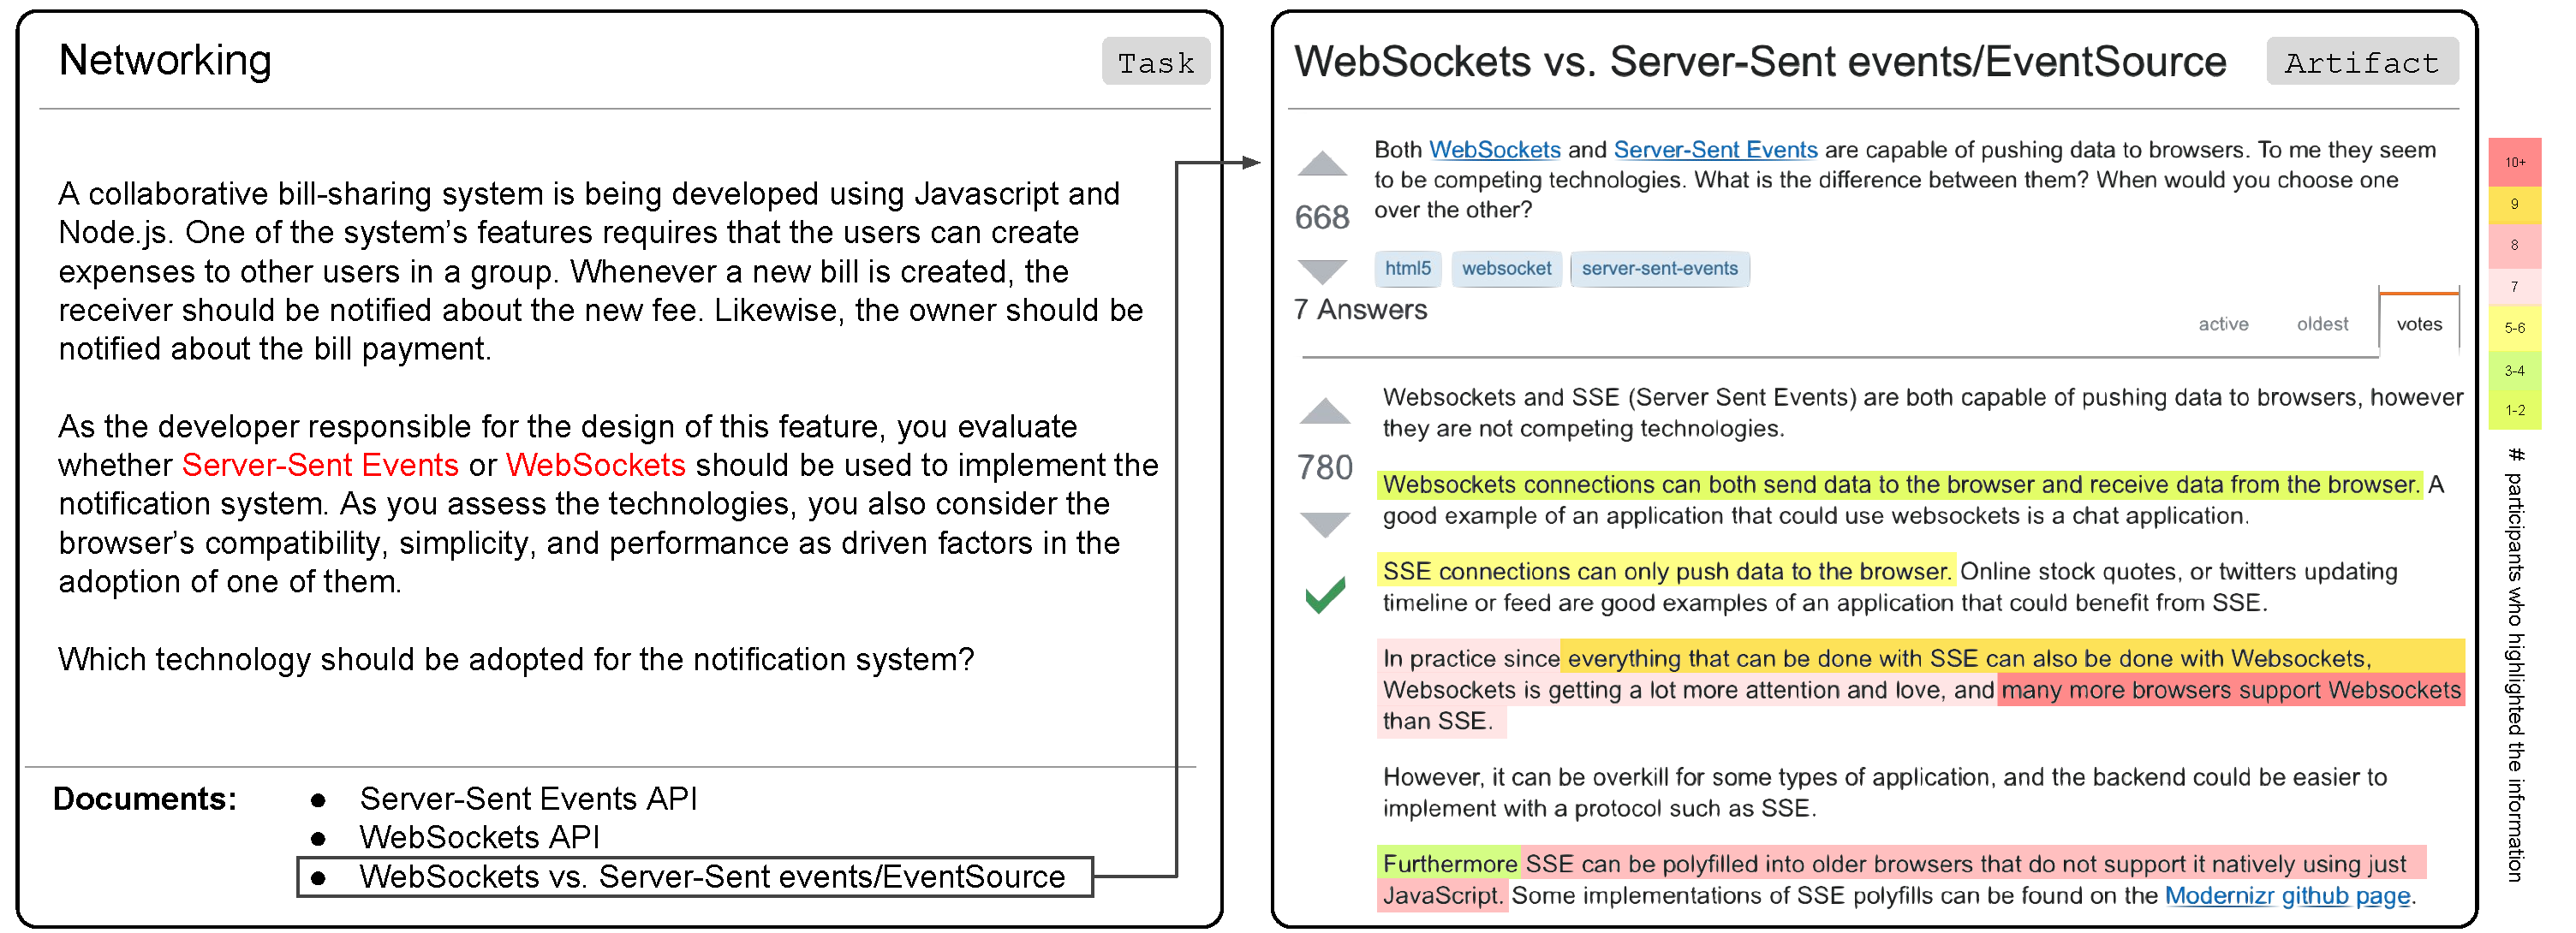
\includegraphics[width=1\textwidth]{cp3/heatmap}
\caption{An example of a task description and a depiction of collected data, shown as a heatmap of text that participants highlighted as relevant to the task}
\label{fig:task-highlights-heatmap}
\end{figure}
% \end{landscape}









\section{Results}
\label{cp3:results}


In this section, we present results first describing the data produced
and 
then, analyzing properties of the text considered relevant. 
We also report results from our interview analysis.





\subsection{Relevant Text in Natural Language Artifacts}




To characterize the task-relevant text found in natural language 
software artifacts (\textit{RQ1}), 
we analyze the participants' produced highlights.
We focus
our analysis on highlights participants made of natural language
text. We do not
consider highlights participants made of source code snippets or in
tables, leaving the consideration of this information to future work.



We define a \textbf{H}ighlighted \textbf{U}nit (HU) as the full sentence containing any
highlight by a participant. 
We use sentences as the unit of analysis 
because this was the most common unit considered by the participants.
That is, of the 2,463
distinct highlights created by participants, 1,777 are sentences
(72\%), 621 are portions of sentences (25\%) and 65 are combinations
of consecutive sentences (3\%). 
Thus, if a participant highlighted just a
phrase in a sentence, we consider the full sentence as an HU or if a
participant highlighted more than one portion of a sentence we still
consider the full sentence as one HU. 


\subsubsection{How much text in an artifact is deemed relevant to a task?}
\label{cp3:ratio}




We first ask how much text within an artifact participants found relevant to a task
since if almost all of the text  is relevant then there would not be a need for
identifying text within an artifact.
Figure~\ref{fig:task-artifact-ratio} presents the ratio of relevant text in each type of document.
We compute the average ratio of HUs and text for each  artifact from each type of document.
We report the mean of the ratio artifact-wise to prevent misinterpretations due to outliers,
i.e., a lengthy document with few HUs or a document concentrating almost all the HUs






Considering all HUs, between 1\% to 20\% of an artifact's text is considered relevant, depending on its type.
API documents have the smallest ratio of
relevant information (mean of 3\%) and for this kind of artifact,
at most 6\% of all sentences were considered relevant.
This result is not surprising as API documents may describe many API features or
methods of which only a few are likely to apply to
a particular task~\cite{robillard2011field}.
% Such quantitative analysis provides further
% evidence supporting qualitative research on API
% documentation obstacles.
% Most notably, that the structure of APIs
% and boilerplate text can bloat the documentation~\cite{robillard2011field, Aghajani2019}.
Similarly, only a small portion (4\% on average) of
the content of 
bug reports are considered relevant.
This result is also not
surprising as bug reports can contain long discussions encompassing
several topics~\cite{Breu2010, Rastkar2010}.
Even the kind of document with the highest
percentage of highlights, Q\&A entries with, on average, 11\%
of the sentences being relevant,
contain a substantial amount of information not relevant to a
specific task. 



\rev{When we look at the amount of information sought for task completion (\textit{RQ1}), our results suggest that:}


\medskip
\begin{bluequote}
    \textit{Finding task-relevant information in a bug report,
    API document and Q\&A documents require filtering to less than
    a 20\% of the document's text.}
\end{bluequote}



\begin{figure}
    \centering
    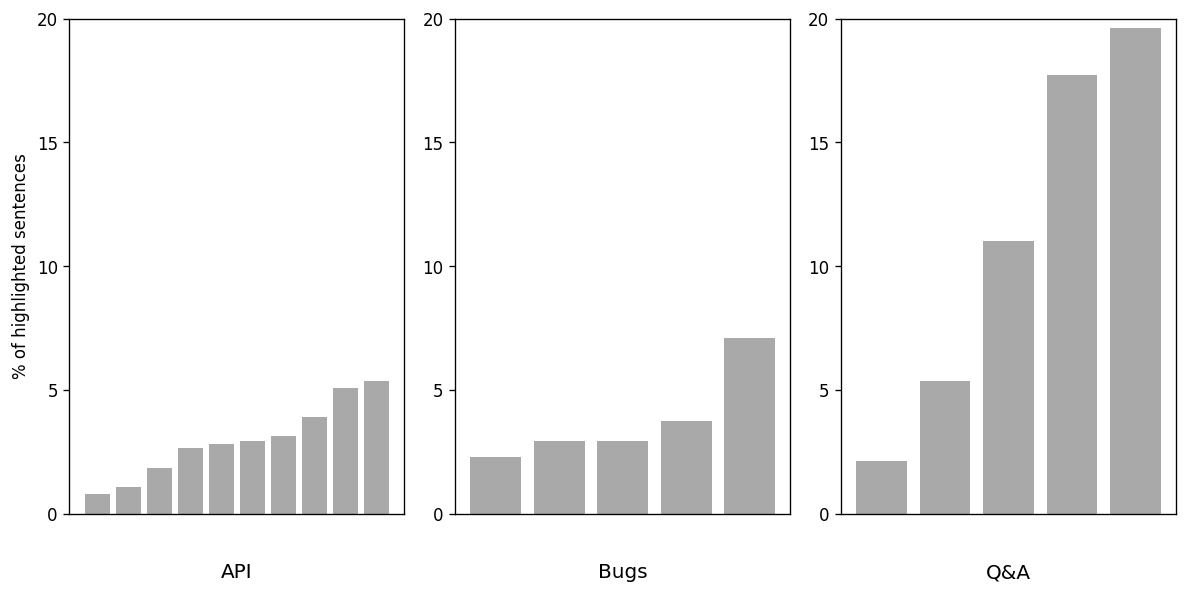
\includegraphics[width=.98\textwidth]{cp3/task-artifact-ratio}
    \caption{Percentage of highlighted sentences per artifact grouped by artifact's type}
    \label{fig:task-artifact-ratio}
\end{figure}

\subsubsection{How much agreement is there between participants about the text relevant to a task?}
\label{cp3:agreement}


With this question, we seek to identify if there is a set of key sentences that
participants unanimously consider relevant to a task. 
We use Nenkova and Passonneau's
pyramid method~\cite{Nenkova2004}
to investigate the degree to which participants agree upon
the text relevant to a task. This method was originally used
to quantify the content of summaries produced by different annotators.
The more annotators who include the same content in their summaries,
the more consistent the view of information relevant to a summary and
the more weight is given to the selected content. We apply the same rationale
to assess the level of agreement of which HUs are relevant to a task
and whether agreement relates to how correctly
a participant completes a task.




% To construct the pyramid, we assign a weight to each HU
% corresponding to the number of participants who highlighted that HU during
% a task.
% From the 602 HUs, we observe that 18\% of them are considered relevant by eight or more participants while 58\% are relevant to only one or two participants.
Figure~\ref{fig:highlights-distribution} shows the distribution of HUs over the pyramid we produce using the pyramid method.
To facilitate interpreting the results,
we take into consideration how other studies provide categories for the relevance of
text (i.e.,~\cite{Petrosyan2015} and~\cite{Jiang2017}) and 
we aggregate HUs selected by a range of participants into three tiers.
Table~\ref{tbl:task-hu} presents HUs per tier.
Starting from the bottom tier, the pyramid represents the perceived relevance of information from less to more relevant.


We use the aggregated data (Table~\ref{tbl:task-hu}) to test if the number of HUs identified at each tier affects how correct were the solutions provided by the participants (as measured by the questionnaires applied for each task). 
Since we have three independent variables (i.e., tiers) and one outcome variable (i.e., scores),
we use a multivariate analysis of variance to test this hypothesis~\cite{wohlin2012}. 
Results indicate a significant differences ($p\text{-value} < 0.01$) between participants' score and their HUs.
We then conducted univariate tests on each tier,
finding that 
the number of HUs identified at the mid and top-tiers 
positively affect the correctness of a participant's questionnaire answer, 
suggesting that HUs from these two tiers contain key
information for completing a task.
As expected, HUs at the bottom tier vary more per participant.
Due to such variability, there is no clear indication
that bottom tier HUs are from participants from a certain group, such as all those
unfamiliar with a particular technology or  who successfully
completed a task and those who did not (Section~\ref{cp3:threats} details threats for this analysis).







\begin{figure}
    \centering
    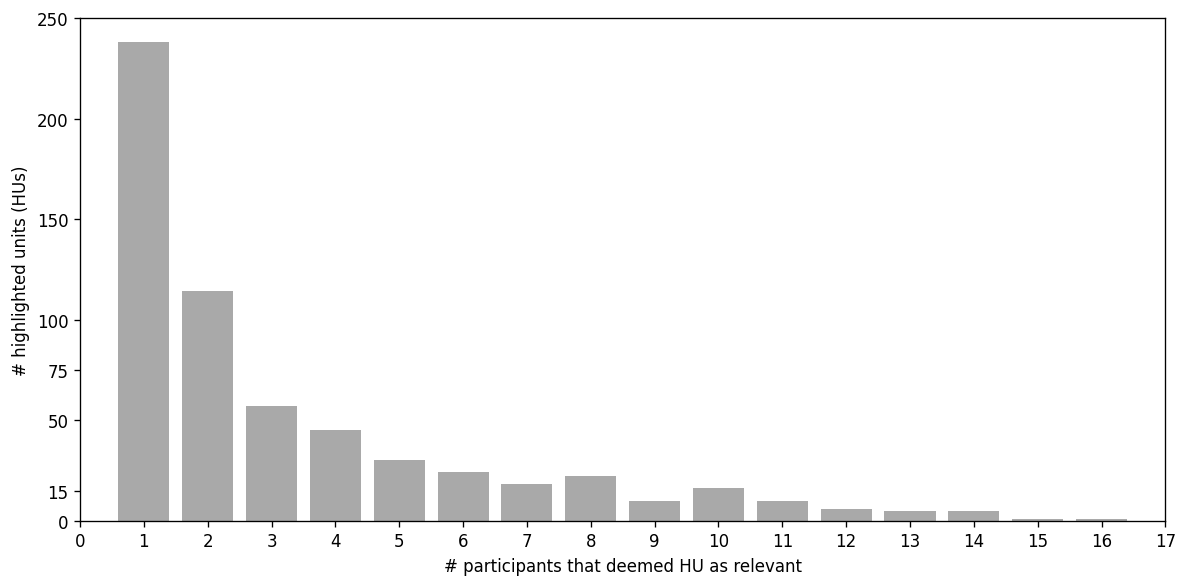
\includegraphics[width=.95\textwidth]{cp3/highlights-distribution}
    \caption{Distribution of the number of participants who deem an HU as relevant}
    \label{fig:highlights-distribution}
\end{figure}




\input{sections/cp3/tables/task-hu.tex}



\rev{When we consider variations in the portion of the text deemed relevant (\textit{RQ1}), we find that:}


\medskip
\begin{bluequote}
    \textit{Text perceived as relevant by more participants likely relates
    to key information for completing a task whereas information
    highlighted by a few participants may be more dependent on the knowledge of individuals.}
\end{bluequote}


\subsection{Textual Evaluation}


We examine syntactic and semantic properties 
of the highlighted text so that 
we might identify
common cues to the relevancy of text to a task (\textit{RQ2}).
Since we intend to use these cues 
in the design general technique, 
we examine the text across 
all the kinds of artifacts 
available for all the tasks. 




For our syntactic analysis,
we start by inspecting the elements that compose a sentence (i.e., nouns and verbs)
using the Python NLTK API\footnote{https://www.nltk.org/} with the CoNLL-2000 corpus~\cite{Conll2000} to automatically extract such data.
We then analyze possible patterns that may arise from the syntactic structure of the text~\cite{Robillard2015}
as well as the syntatic dependencies between verbs and  other elements related to them~\cite{Chaparro2017}, investigating if the extracted entities co-occur in multiple HUs. 
For instance, consider the sentence:
``\textit{you can use include\_fields if you want specific field names}''.
We can extract the elements dependent upon the the verb `\textit{use}' (i.e., {\small \texttt{[nsubject, use, code\_word]}})
and, if we observe that these elements co-occur in multiple HUs, we flag the pattern as a cue to the relevancy of the text.





As for semantics, we
analyze HUs for \textit{semantic
frames}~\cite{fillmore1976frame}
using frame semantic parsing~\cite{Baker1998, jurafsky2014speech}.
Semantic frames are centered around events, capturing both the event
as well as relationships, entities or participants related to that
event~\cite{fillmore1976frame, Baker1998frame}. 
We explain semantic frames by considering the application
of semantic parsing to two distinct sentences extracted 
from the \texttt{Databases} and the \texttt{Lucence} tasks, respectively.
For each sentence, Figure~\ref{fig:frame-examples} shows an
excerpt of the frame analysis for the sentences. 
The frames of each sentence (in grey) represent a triggering event and the frame elements \textit{(fe)} (in red) are arguments needed to understand the event. The enclosing square brackets mark all lexical units, or words, associated with either a frame or a frame element.

\medskip
\input{sections/cp3/semantic-frames-example}


Observing the frame elements captured by the verbs \textit{see} and
\textit{understand}, both sentences have the common meaning of
describing a `\textit{phenomenon}'.
However, the frame elements
that capture the meaning of each verb differ: the former represents a
`\textit{perception of experience}' while the latter represents a
cognizer `\textit{grasp}'ing her knowledge over the 
phenomenon. 


As multiple sentences might have similar meanings,
we analyze whether there are common frame elements 
that provide cues to the relevancy of text.
For this analysis, all frame elements were extracted automatically.
We decompose HUs to obtain the semantic frames for the sentence 
using the \textit{SEMAFOR} toolkit~\cite{das2014frame}.
For a detailed definition of each frame, refer to
the FrameNet
database\footnote{https://framenet.icsi.berkeley.edu/fndrupal}.




\subsubsection{Does syntactic structure provide cues to the relevancy of text to a task?}
\label{cp3:syntactic-analysis}



We start our syntactic analysis by describing noun phrases and verb phrases
in the relevant text. 
We then describe our analysis of syntactic patterns.  



Among noun phrases, we observe that 65\% of the HUs contain acronyms or coding elements.
Existing approaches that rely on these elements to identify relevant text (e.g.,~\cite{Robillard2015} or~\cite{Jiang2016b}) would miss the remaining 35\% of the HUs in our corpus.
This value may seem acceptable at first; however there are no guarantees that
the identified 65\% HUs hold all the crucial information for task completion.
As an example, some of the HUs from the mid and topmost tiers 
do not contain obvious code words that could signal their relevancy,
such as one of the sentences in the \texttt{Bugzilla} task indicates the need for ``\textit{authentication to allow retrieving non-public data}''.
% The lack of authentication implies missing non-public data, which leads to an incomplete solution, 
% and so this sentence was considered relevant by most of the participants in our study
% even when it .





With regards to verb phrases, we observe a substantial
overlap (81\%) with verbs observed in Ko and colleagues linguistic analysis
of bug report titles~\cite{Ko2006}.
The most common verbs in the HUs include conjugations of verbs such as \textit{use}, \textit{get}, \textit{set}, \textit{be}, or \textit{do},
but with the exception of \textit{use}, \textit{get}, and \textit{set}, the
remaining top common verbs are in English stop words lists~\cite{jurafsky2014speech}. As a result, many
\acs{NLP} techniques would discard them as part of their pre-processing
steps~\cite{Bavota2016}.






As for syntactic patterns, we did not observe a large set of patterns for the variety of tasks and artifacts in our experiment,
where the prominent patterns identified (e.g., \texttt{[nsubject, do, negation]})
reflect common constructs of the English language rather than cues that we might explore for the relevancy of text.
There may be multiple explanations for these results, such as
the fact our corpus contains a small number of natural language artifacts.
Due to this reason, we also checked whether patterns from existing related work (i.e.,~\cite{Chaparro2017, Robillard2015}) applied to the text in our HUs, 
but the small number of matching patters 
raises caution on
their generalizability.



\medskip
\begin{bluequote}
    \textit{We did not find prominent syntactic cues to identify
    task-relevant information. Our analysis of highlights demonstrates:
    1) limitations of existing techniques that rely on code
    words and acronyms, 2) missed
    information that may occur due to the prevalence of verbs that
    appear in English stop word lists,
    and 3) the absence of patterns derived from the syntactic structure of
    the text.}
\end{bluequote}

 



\subsubsection{Do semantics provide cues to the relevancy of text to a task?}
\label{cp3:semantic-analysis}


We extract the frames of every HU, resulting in 3,719 frames across
the 602 HUs. Only 346 distinct frames appear across these 3,719 frames
parsed. The proportionally small number of distinct semantic frames
occurring
suggests that different HUs share frame elements. 



Table~\ref{tbl:common-frames} details the most frequent frames identified per tier, filtering to show the 
most frequent frames in a tier that have not appeared in lower tiers.
In the top-most tier, the most frequently identifying distinguishing
frames denote the \textit{cause} or \textit{likelihood} of a phenomenon.
These frames are found in sentences that explain a system's behavior, which are often crucial for task completion,
as in a sentence that provides a cause for the loss in performance when using Hibernate:
 \textit{``if you need to process lots of objects for some reason, though it can seriously affect performance}''.
Other common frames \textit{quantify relationships},
as when a sentence describes the minimum elements needed to perform an operation, e.g., \textit{``to create a flag, at least the status and the type\_id or name must be provided}''.




In the middle tier, we observe frames for actions performed by some entity (\textit{intentionally act}) or facts regarding a topic (\textit{statement}).
Other common frames relate to methods or attributes and the result of some operation such as a method call, which may be useful for identifying code related entities.
For instance, this sentence from the \texttt{Bugzilla} tasks contains both the \textit{being returned} and the \textit{fields} frame, 
\textit{``You can specify to only return custom fields by specifying \texttt{\_custom} or the field name in \texttt{include\_fields}''}.



\input{sections/cp3/tables/common-frames}


The bottom tier contains frames that are common to all HUs.
The most frequent frame in the bottom tier has a semantic meaning of \textit{using}.
HUs with this frame are often sentences detailing how to use a method or a
framework to achieve some goal, what might also explain the second most frequently occurring frame, i.e., \textit{purpose}, which denotes an achievable goal. 
These two frames could be used to filter sentences that contain the means
to use a technology or API with certain intention, as this sentence explaining usage scenarios for
WebSocket and Server-Sent Events in the \texttt{Networking} task:
``\textit{One is synchronous and could/would be used for near real-time data xfer, whereas the other is asynchronous and would serve an entirely different purpose}''.





To further characterize  frame elements, 
we pairwise compare their frequency in relevant text (i.e., HUs) and non-relevant text.
Figure~\ref{fig:frame-distribution} provides insight in the distribution of frames across relevant and non-relevant sentences.
We perform a Wilcoxon signed-rank test~\cite{wohlin2012} over the distribution of frames in our data and we observe with statistical significance ($p\text{-value} \le 0.05$) 
that certain frames are more prominent in relevant or non-relevant sentences.
For example, frames that represent a \textit{required} event
are more prominent in the relevant text
as found in a sentence in the \texttt{Bugzilla} REST API that describes
how to circumvent errors due to invalid tokens:
``\textit{An error is thrown if you pass an invalid token; you will need to log in again to get a new token}''.
On the other hand, frames that relate to user discussions and that do not draw conclusions or provide 
facts about an API or technology, such as \textit{point of dispute} or \textit{reasoning} are often found in non-relevant text,
as when users discuss community's procedures in the \texttt{GPMDPU} task: ``\textit{Open a new issue following the template so we can have more details on your device}''. 




\begin{figure}
\centering
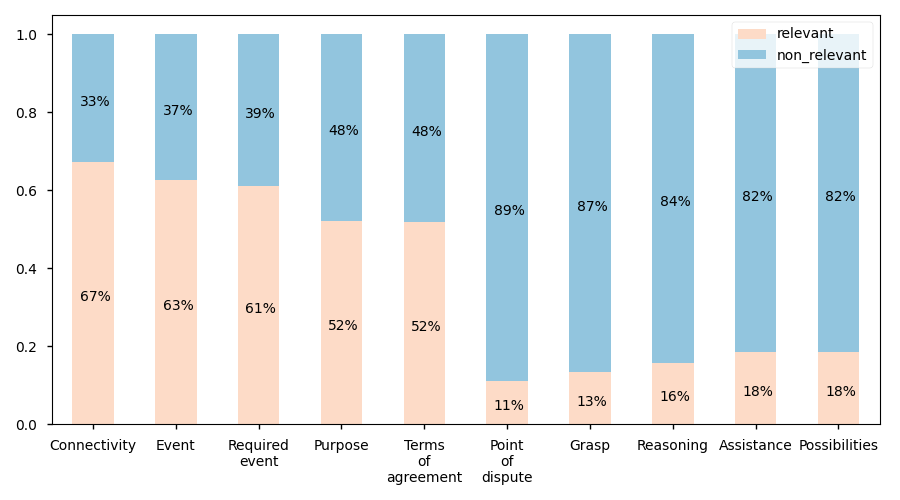
\includegraphics[width=.95\textwidth]{cp3/frames-dist-all}
\caption{Distribuion of semantic frames over the text; the figure depicts the top five frames most commonly observed in relevant and non-relevant sentences, respectively}
\label{fig:frame-distribution}
\end{figure}


While certain frames are not indicative of relevance when found on their own, we also observe that the co-ocurrance of certain frames in a sentence increase the likelihood of the sentence's relevancy.
For instance, \textit{purpose} and \textit{using} occur almost evenly across relevant and non-relevant text
while their co-occurrance is more frequent in relevant text. 
Figure~\ref{fig:frame-co-occurrence} shows the most frequent frames that co-occur and their ratio on relevant and non-relevant text.



\begin{figure}
\centering
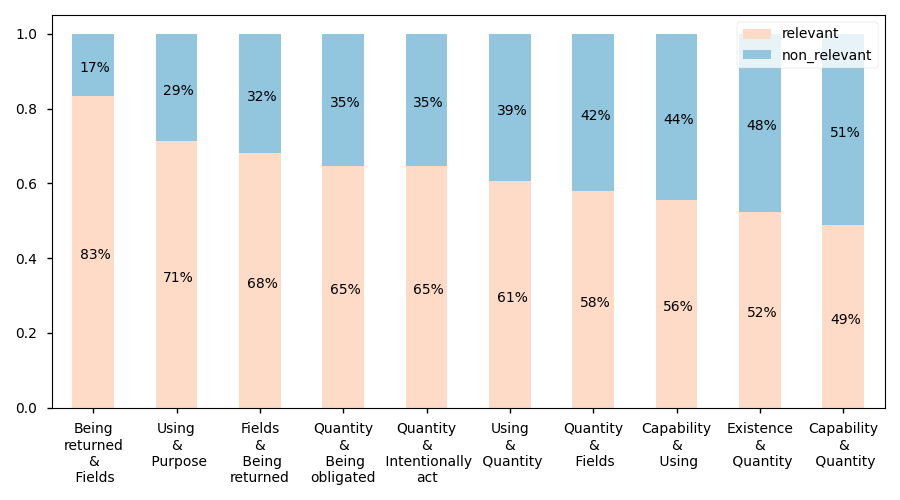
\includegraphics[width=.95\textwidth]{cp3/frames-dist-2-grams}
\caption{Distribution of co-occurring frames over the text}
\label{fig:frame-co-occurrence}
\end{figure}


Our analysis on the semantics of relevant text indicates that there exists some common aspect to the different sentences deemed as relevant.


\medskip
\begin{bluequote}
    \textit{There are recurring semantic meanings in relevant sentences,
    suggesting commonalities in their conveyed information
    and indicating that text might be identified through its semantics.}
\end{bluequote}


\subsection{Interview Analysis}

To understand how participants identified relevant text (\textit{RQ3}), we analyzed the participants'
interview responses using a card-sorting approach~\cite{spencer2009sorting}.
We\footnote{The first two authors of~\cite{marques2020}: A. Marques and N. C. Bradley} created index cards containing the interview questions and the participants' responses.
The cards were sorted into meaningful themes and then grouped into abstract categories.
We refined themes over three iterations of the data.
At each  iteration, we grouped cards containing responses on similar topics, analyzed the emerging theme, and evaluated
whether there was a broader theme that incorporated two or more of the existing themes.
To reduce individual bias, the researchers involved in this analysis independently annotated a subset of the cards at every iteration.
Disagreements occurred when more than one theme could apply to a sentence.
The annotators discussed and resolved disagreements refining the set of themes in a subsequent iteration, reaching substantial agreement ($\kappa=0.82$).





From participants' comments, we identified nine themes that we group under two major categories.
Table~\ref{tbl:themes-categories} details observed categories, themes, and the number of participants who made a comment pertaining to that theme.
We discuss results per category illustrating comments that best exemplify a theme. To facilitate the discussion we highlight themes (in gray)
when we first mention them.



% This analysis led us to a final set of nine themes (Table~\ref{tbl:themes-categories}). We discuss these themes (grey highlights) grouping them under two major categories: \textit{Search strategies} and \textit{Search challenges}.


\afterpage{
\input{sections/cp3/tables/card-sorting-themes.tex}
}



\subsubsection{How do developers locate relevant information?}
\label{cp3:search-strategies}

Developers often use a mix of \hl{\textit{keyword-matching}} and \hl{\textit{skimming}}~\cite{Starke2009, Ko2006a} to find relevant information within an artifact. 
Some participants said they use these search strategies for all types of artifacts, while others said they use knowledge of a document's structure to assist their searches (\hl{\textit{document-guided}}).


% \pquote{}{P12} \medbreak

\smallskip
% \begin{footnotesize}
\begin{quote}
    ``\textit{Definitively [my strategy] wasn't always the same. Going through a StackOverflow question, I would obviously read the first response. For API docs, keywords were the go to. Bug reports are hard. Comments are ordered chronologically and the first ones are sometimes not the most relevant ones}''---P12
\end{quote}
% \end{footnotesize}


Participants were also aware of the shortcomings of some artifact types and were less willing to use faster but less accurate strategies like skimming or keyword-matching for these artifacts when the tasks were difficult. 
In these cases, participants mentioned that they used a \hl{\textit{scrutnizing}} strategy:


\smallskip
% \begin{footnotesize}
\begin{quote}
    ``\textit{I usually read every comment [on StackOverflow]. Obviously, they are ranked, but, in general, every single comment could have something important}''---P11
\end{quote}
% \end{footnotesize}
    


Regardless of strategy, participants mentioned using 
implicit criteria to decide when to (not) read some text.
Such implicit criteria often relate to information foraging theory (Section~\ref{cp2:searching}) and how an individual follows some
\hl{\textit{information scent}} for judging the cost of investigating some text according to available cues~\cite{Pirolli1999}, such as the presence of bullet-points, bold text, or the conciseness and readablilty of the text.



\subsubsection{What challenges do developers face while searching for relevant information?}
\label{cp3:search-challenges}


Participants also commented on factors that made assessing the relevancy of text difficult.
The most common challenge was \hl{\textit{missing information}} that other participants deemed relevant.



\smallskip
% \begin{footnotesize}
\begin{quote}
    ``\textit{This [highlight] is a valid alternative if you don't want to use the conflicts [method]. I basically didn't see this because of how I was searching}''---P2
\end{quote}
% \end{footnotesize}




We consider missing relevant information as a major threat to task completion because it can lead to an incomplete or incorrect solution~\cite{Murphy2005};
usually, participants missed information due to their workflows, as \textit{P15} explains:





\smallskip
% \begin{footnotesize}
\begin{quote}
    ``\textit{It's hard to say that I would have picked [those highlights] without being directed to that. I believe that I knew that there were specific questions coming, but even if I was doing it for myself, I would probably skim first and then, when I start to code, it would be a natural thing to get back and dive into the details}''---P15
\end{quote}
% \end{footnotesize}



Participants also missed information due to text \hl{\textit{verbosity}}. 
Bloated text makes it harder for developers to locate task-relevant information~\cite{robillard2011field} as it is more cognitively demanding to read verbose text:


\smallskip
% \begin{footnotesize}
\begin{quote}
    ``\textit{When I looked at the API documentation, there was too much text. I was mentally exhausted just looking at it}''---P6
\end{quote}
% \end{footnotesize}


Participants noted that their \hl{\textit{familiarity}} with the task domain also affected how they located relevant information in the text.



\smallskip
% \begin{footnotesize}
\begin{quote}
    ``\textit{The easiest one was the one about ORM/JDBC [databases] because I was so familiar with these technologies}''---P2
\end{quote}
% \end{footnotesize}




Finally, when presented with \hl{\textit{ambiguous or contradictory}} information, participants had to spend time seeking out additional information to resolve the ambiguity.


\smallskip
% \begin{footnotesize}
\begin{quote}
    ``\textit{I think it was in this one [highlight]. They said that \texttt{cmd} works in the same way as \texttt{Ctrl}, but I went with the one that says otherwise. [...] it was actually helpful to have two other highlights so I had a bit more reliance on the thing that was mentioned by more users.}''---P19
\end{quote}
% \end{footnotesize}



Our analysis on the participants' comments on their search strategies provides further insights into how developers forage for information in software development natural language artifacts. One of our key observations is that  developers use mixed strategies to locate task-relevant information. In doing so, developers often miss some information that might be relevant to the task that they are performing.


\medskip
\begin{bluequote}
    \textit{Developers use mixed strategies to locate task-relevant information, often missing some information that might be relevant to complete a task completely and correctly.}
\end{bluequote}




\subsection{Summary of Results}


The results we obtained 
from the analysis of highlights produced by 
developers inspecting artifacts 
pertinent to six software tasks indicate that
between 1\% to 20\% of the text of an artifact was considered
relevant to a task.
While we failed to observe syntactic cues 
that could indicate the relevance of text to a task, 
we observe consistency in the meaning of the relevant text---as captured using frame semantics---suggesting that semantic-based approaches 
may be more appropriate for the 
automatic identification of task-relevant text.




\subsection{Threats to Validity}
\label{cp3:threats}


In this section, we discuss threats from our experimental design 
and from our
examination of the relevant text (HUs) produced by participants who 
inspected natural language artifacts from six information seeking tasks. 



The design of the six tasks in our experiment represents a threat to
\textit{construct validity}.  To mitigate this threat, we used results from studies discussing the search
behaviour of developers~\cite{umarji2008archetypal, Li2013, Xia2017} as
input to the design of our tasks.
For each task, our goal was to provide a set of artifacts so that a
participant could gather enough knowledge to complete the task, which
we confirmed through pilot studies.  The provision of artifacts was also
necessary to enable a systematic analysis of relevance through a
controlled experiment. We mitigated threats on artifact
selection by asking external researchers to provide their own list of
candidate artifacts, which was similar to our own list.



The \textit{external validity} of the experimental results is affected
by the participants, the tasks and the artifacts.  Considering the
subjective nature of relevance, the knowledge and particularities of
our participants may not generalize to other software developers.
Furthermore, the structure and linguistic characteristics of the
artifacts considered may not extend to other kinds of artifacts or the
same kind of artifacts in other domains.  We tried to mitigate this
threat by selecting different kinds of artifacts such as API
documentation, bug reports, and Q\&A pages while 
ensuring that each kind was present in at least
50\% of the tasks. 
However, our results
are bound to the domains and artifacts we evaluated and may not generalize.
Future work should confirm our findings on a wider range of artifacts and tasks.


There are also threats to the validity of our
\textit{conclusions}.
Experimental procedures encouraged participants to work on the tasks using their normal workflow.
However, at least one participant (\textit{P15}) indicated that they would normally
revisit a document as different information needs arise as part of a task.
As a result, our study may miss relevant information.
In addition, the text participants highlighted may not have always aligned with the text that contained information useful for completing the task.
To investigate this alignment further, we would have had to create an oracle containing the relevant text.
Unfortunately, creating the oracle is challenging because it would need to encompass different perceptions of relevance~\cite{Pirolli1999,saracevic1975,Nenkova2004} and usefulness~\cite{Freund2013, Freund2015}.
Thus, to avoid the subjective and imprecise process of judging alignment, we simply consider any text highlighted by participants as containing information useful to completing the tasks.



While the size of our corpus might also affect our conclusions,
we emphasize that the HUs from mid and top-tiers in our data comprise 250 sentences, 
which is similar to the amount of data studied previously. For instance, the McGill~\cite{Petrosyan2015}
and Android~\cite{Jiang2016b} datasets contain 238 and 141 relevant text fragments, respectively.


To extract the meaning of text through parsed frames, 
we used a general frame semantics database rather than one
specific to software engineering.  This led to frames that were
\textit{out-of-context}, causing us to adapt either the frame's
name or its description.  
Frames adapted to software engineering (e.g., \textit{being returned}
and \textit{fields}) represent a small fraction of all the extracted
frames. As a result, we argue that all the sentences containing them still have
similar semantic meanings and our conclusions are not
affected by these out-of-context frames. However, as we discuss in Chapter~\ref{ch:discussion}, 
having specific
software engineering frames could improve our results.




% \subsection{Summary of results}



\section{Summary}
\label{cp3:summary}



In this chapter, we addressed the problem of locating relevant information
to a particular software development task \textit{within} a natural language artifact.
To better understand how relevant information is encoded in natural language artifacts,
we detailed an empirical study investigating what text is perceived as relevant
and whether there is consistency in what 20 participants with software development experience deem relevant
to a particular software development task.


Our study comprised the analysis of a set of 20 artifacts originating from API documentation, bug reports, and Q\&A documents.
We observe that finding task-relevant information in such artifacts requires filtering to less than
a 20\% of the documents' text and that there is substantial variability in what information participants perceive as relevant.
Nonetheless, there are commonalities shared through most of the identified relevant textual pieces.
These commonalities are found in the semantic meanings extracted from the text suggesting that
the semantics of natural language artifacts  
can be used in automatic approaches for identifying task-relevant text.




% \clearpage

% H18-02104

% 	Task Knowledge Extraction

% \setcounter{chapter}{3}
\setcounter{rq}{1}


\chapter{Identifying Task-Relevant Text}
\label{ch:identifying}


\stepcounter{rq}

\vspace{1mm}

\begin{enumerate}[label=\textit{RQ\arabic*},leftmargin=1.4cm]
\setcounter{enumi}{\the\numexpr \arabic{rq} - 1\relax}

\item \textit{What techniques can we use to automatically extract text relevant to a software developer's task?} 

\end{enumerate}

\vspace{1mm}

--- Chapter introduction 

------ Use findings of characterization studies (cp3) to motivate the need for the techniques proposed in this chapter

------ Brief summary of techniques we propose

------ Brief summary of evaluation and results



\clearpage


\section{Approach}
\textcolor{white}{force ident} % this is just for the chapter outline

--- We address the problem of automatically detecting task-relevant text in a \textit{artifact-agnostic} way. \vspace{3mm}

--- To design our approaches, we use the manually curated task-relevant sentences produced in our characterization study~\cite{marques2020} \vspace{3mm}

--- We investigate two main approaches:

------ \textit{Heuristic-based}: uses a set of properties in the text (including \textit{semantic frames}~\cite{fillmore1976frame}) to determine if a given sentence is relevant to the input task

------ \textit{ML-based}: uses the novel \textit{Transformer}~\cite{Vaswani2017attention} neural network to jointly model the relevancy of a given input sentence with respect to a task. 

--- Explain why we have selected these two approaches

------ With our first approach, we investigate whether a light-weight technique addresses the need of automatically identifying task-relevant text, what could potentially discourage the need for more complex and computationally expensive solutions~\cite{Bavota2016}

------ Our second approach investigates the applicability of pre-trained models that do not require large amounts of training data to our domain problem~\cite{devlin2018bert, Ye2016}. With this approach, we revisit findings on the trade-offs of using machine learning techniques to mine textual data~\cite{Chaparro2017, Bavota2016}.



\clearpage

\section{Task-pertinent Artifacts Corpus}
\textcolor{white}{force ident} % this is just for the chapter outline

--- To evaluate the techniques proposed in this chapter, we require a sufficiently large corpus containing 
software tasks and associated artifacts originating from heterogeneous sources.
Unfortunately, such a corpus is not promptly available and thus, 
this section outlines the steps we took for its creation.


\section{Software Tasks}
\textcolor{white}{force ident} % this is just for the chapter outline

--- We consider a software task as a piece of work undertaken by a developer that often has to be finished within a certain time~\cite{2004merriam}. 
Two common places a software task can be found are:

\begin{itemize}
    \item the description of a bug or feature request reported in a bug tracking systems; or in
    \item a post in a community forum, development mailing lists, and others.
\end{itemize}

\vspace{3mm}

--- Given this definition, we select tasks from StackOverflow and GitHub to build our corpus

------ We scope task selection to the \textit{Android} development domain such that we can select common tasks across the two sources \vspace{3mm}



--- Detail that StackOverflow tasks were selected from Baltes et al. dataset~\cite{baltes2019-rep}

------ Give example of a StackOverflow task \vspace{5mm}

--- Because there is no GitHub dataset promptly available, we selected GitHub issues from top starred Android projects on GitHub 

------ Projects were selected among Open Source Systems that had the \textit{Java} and \textit{Android} tags. 

------ We randomly sampled 15 issues from a total of 10 distinct projects

------ Describe how we avoid common pitfalls  when mining GitHub~\cite{kalliamvakou2014}

------ Give example of a GitHub task 

\section{Artifact Selection}
\label{cp4:corpus-artifacts}
\textcolor{white}{force ident} % this is just for the chapter outline


--- Our artifact selection approach seeks to simulate everyday practices on how developers search the Web~\cite{rao2020, Xia2017} \vspace{3mm}

--- To that end, we consider a task's title (i.e., SO question or GitHub issue title) as the seed used to search for pertinent artifacts in a search engine

------ This is a common procedure adopted by many studies in the field (e.g.,~\cite{Xu2017} or ~\cite{Silva2019}). \vspace{3mm}


--- As there are many different sources of artifacts, we restrict artifact selection to well known and studied sources~\cite{Starke2009,Kevic2014, Li2013}:


\begin{itemize}
    \item Android and Java SE API documentation;
    \item Github issues;
    \item StackOverflow answers; and
    \item Websites from the java and android categories on Alexa~\cite{alexa}.
\end{itemize}


\vspace{3mm}

--- For these sources, we use the \texttt{googlesearch} API~\cite{googlesearch} to perform Web searches

------ Results were limited to English and a maximum of 5 resources per source 

------ These limitations were necessary because of throttling or even blocking mechanisms in the APIs used the fetch data in each of the sources considered \vspace{3mm}

--- Provide descriptive statistics for the corpus

------ 300 tasks, 150 from SO and 150 from Git

------ Approximately 2,500 artifacts

------ Almost 260,000 sentences

\clearpage


\section{Analytic Evaluation}
\textcolor{white}{force ident} % this is just for the chapter outline

--- To be able to judge the accuracy of any technique used to automatically identify sentences relevant to a task,
we require test data comprising sentences that contain information needed for task completion. \vspace{3mm}

--- We rely on human experts to produce this data \vspace{3mm}


--- With the experts data, we report a technique's accuracy for the given task and artifact source

------ For sources that have been evaluated in other studies, i.e., API documentation~\cite{Robillard2015}, GitHub issues~\cite{Lotufo2012}, and StackOverflow answers~\cite{Xu2017}, we compare the accuracy of our techniques 
to the state-of-the-art

------ To show that our techniques extend beyond well known/studied sources, we also report our techniques accuracy on miscellaneous sources, e.g., Websites from Alexa



\subsection{Golden Standard}
\textcolor{white}{force ident} % this is just for the chapter outline

--- Creating test data for the entirety of our corpus is infeasible so we restrict our evaluation to a subset of 10 tasks evenly sampled from the two types of tasks in the corpus (i.e., 5 GitHub tasks and 5 StackOverflow tasks) \vspace{3mm}

--- For these tasks, golden data consists of any sentence that two or more experts have deemed as useful for task-completion \vspace{3mm}



\subsubsection{Annotators}
\textcolor{white}{force ident} % this is just for the chapter outline

--- We recruited \red{n} graduate students with professional programming experience to produce \textit{golden} data for these 10 tasks. \vspace{3mm}


\subsubsection{Annotation Procedures}
\textcolor{white}{force ident} % this is just for the chapter outline

--- Our intention is that goldens reflect text that an \textit{expert} would deem as useful for task completion. \vspace{3mm}


--- To produce such data, annotators had a set of randomly assigned tasks description and links to artifacts 
pertinent to the respective task at their disposal \vspace{3mm}

--- We asked annotators to write a short comment (250 words max~\cite{Rastkar2010}) with instructions that a newcomer could follow to successfully complete the task.

------ The purpose of the comment was to ensure that annotators built enough context about the task \vspace{3mm}

--- Once the comment was written,  annotators had to manually highlight sentences that they deemed useful and that provide information that assists task completion.

--- Three different individuals performed each task. \vspace{3mm}

--- An in-house tool in the form of a Web browser plugin facilitated annotation procedures

\subsection{Method}
\textcolor{white}{force ident} % this is just for the chapter outline

--- For each task, we have a set of artifacts with sentences identified by experts that contain information relevant to the task \vspace{3mm}

--- For each task and artifact type, we apply the appropriate technique (baseline and ours) to automatically detect task-relevant text in that artifact

--- We then compute the technique's accuracy against the experts' highlights 

--- We use the obtained values to discuss the accuracy of each technique on their respective artifacts



\subsubsection{Baselines}
\label{cp4:comparison-techniques}
\textcolor{white}{force ident} % this is just for the chapter outline

--- We systematically reviewed related work and we identified techniques applicable to our domain problem

------ Selection criteria considered each technique's availability in existing replication packages and their readiness for use.

------ We also refrained from using approaches with training procedures (e.g., ~\cite{liu2020} or ~\cite{Treude2016}) because of ~\cite{Chaparro2017, fucci2019} \vspace{3mm}


--- Based on these criteria, we selected the following techniques for comparison:


\begin{itemize}[leftmargin=\parindent, font=\normalfont\itshape]
    \item \textit{SO Answers} (\texttt{AnsBot})~\cite{Xu2017} --- short description of the approach;
    
    \item \textit{API Documentation} (\texttt{APIRef})~\cite{Robillard2015} --- short description of the approach;
    
    \item \textit{GitHub issues} (\texttt{HurriedBug})~\cite{Lotufo2012} --- short description of the approach;

    \item \textit{Miscellaneous} (\texttt{LexRank})~\cite{Erkan2004} --- in the lack of an artifact-specific technique for this category, we use LexRank as a baseline because it has been evaluated in several studies that address the identification of textual information in natural language software artifacts~\cite{nadi2020, Ponzanelli2017}
\end{itemize}






\subsubsection{Evaluation Metrics}
\textcolor{white}{force ident} % this is just for the chapter outline

--- We use the golden data to compute precision and recall


--- For a given task $t$ and artifact $a$, precision is computed as the ratio between the sentences identified that are indeed relevant (i.e., sentences identified by the experts) and the total number of sentences identified by the technique


\begin{equation}
    Precision(t, a) = \frac{\# \text{\textit{sentences identified that were marked as relevant by the experts}}}{\# \text{\textit{sentences identified}}}
\end{equation}

\vspace{3mm}

--- Recall represents how many relevant sentences are identified by a technique


\begin{equation}
    Recall(t, a) = \frac{\# \text{\textit{sentences identified that were marked as relevant by the experts}}}{\# \text{\textit{sentences marked as relevant by the experts}}}
\end{equation}

\vspace{3mm}

--- When comparing techniques, we favor precision instead of recall because false positives may contribute to a developer abandoning reading of an artifact that would otherwise provide crucial information for her task~\cite{Rastkar2010}.


\subsection{Results}
\textcolor{white}{force ident} % this is just for the chapter outline

--- Discuss results \vspace{3mm}

\subsection{Threats to Validity}

--- Discuss threats \vspace{3mm}

\clearpage


\section{Human Evaluation}
\textcolor{white}{force ident} % this is just for the chapter outline

\red{argument to justify this second evaluation}

--- Although our analytic evaluation gives insight on how accurately can we identify text relevant to a task within a natural language artifact, we seek to provide further evidence on whether software developers consider automatically detected text as useful for a task 

--- In this study, we asked software developers to indicate if automatically detected text provided important/useful information needed to correctly accomplish a task.

--- This evaluation was performed on a random sample of 30 tasks in our corpus (distinct from the expert tasks)

--- To avoid confirmation biases, developers provided input for both text detected by one of our approaches (i.e., the approach that had the best results in our analytic evaluation) and text detected by approaches in the literature (Section~\ref{cp4:comparison-techniques})



\subsection{Participants}
\textcolor{white}{force ident} % this is just for the chapter outline

--- For this evaluation, we consider the challenges of recruiting software developers in the local area and we instead opt to use 
\textit{Amazon Mechanical Turk}~\cite{mturk} (MTurk).

--- Background questions ensured that individuals had Java development experience and that they had familiarity with the artifact sources in our corpus.

--- Specifically, a MTurk evaluator---\textit{turker}--- had to answer the following background questions:


\begin{enumerate}[leftmargin=\parindent, font=\normalfont\itshape, label=BQ\textsubscript{\arabic*.}]
    \item Is developing software part of your job? Yes, no 
    \item For how many years have you been developing software? Free text
    \item How would you rate your development expertise in Java? No experience at all developing Java, Beginner, Intermediate, Expert
    \item How would you rate your development expertise in Android? No experience at all developing Android, Beginner, Intermediate, Expert
    \item When performing a software task, what sources do you normally seek information on? Multiple choice: API documentation, Stack Overflow, Github, Medium, ...
\end{enumerate}

   

\subsection{Method}
\textcolor{white}{force ident} % this is just for the chapter outline


--- All the evaluation was performed in the Mechanical Turk platform. \vspace{3mm}

--- Turkers indicated the relevancy of a sentence to a given task  by answering the question: \vspace{3mm}

\begin{enumerate}[leftmargin=\parindent, font=\normalfont\itshape, label=SR\textsubscript{\arabic*}]
    \item Which of the following statements best describes this sentence? 
    \textit{(a)} The sentence is meaningful and provides important/useful information needed to correctly accomplish the task in question, 
    \textit{(b)} The sentence is meaningful, but does not provide any important/useful information to correctly accomplish the task in question, 
    \textit{(c)} The sentence does not make sense to me.
\end{enumerate}

--- We deliberately word the question as close as possible to other peer-reviewed studies in the field~\cite{nadi2020, Xu2017}. \vspace{3mm}


--- Due to constraints on the platform, the evaluators judged sentences individually, i.e., without access to the context in which the sentences appeared. \vspace{3mm}

--- Turkers also had to answer a \textit{quality-gate task} randomly drawn from the experts' tasks.

------ The task showed five expert-curated sentences (all marked by the experts as relevant) and a turker had to indicate the sentences' usefulness as in any other task.

------ We discarded responses from any turker who deemed less than three out of the five sentences as useful for the task


\subsubsection{Evaluation Metrics}
\textcolor{white}{force ident} % this is just for the chapter outline

--- We report a quantitative analysis of the ratings provided by the turkers




\subsection{Results}
\textcolor{white}{force ident} % this is just for the chapter outline

--- Discuss results \vspace{3mm}

\subsection{Threats to Validity}

--- Discuss threats \vspace{3mm}

\clearpage

\section{Summary}
\textcolor{white}{force ident} % this is just for the chapter outline

--- Summary of contributions for the chapter \vspace{3mm}

------ A corpus containing 300 software tasks originating from StackOverflow and Github and associated artifacts containing potentially relevant information to correctly completing the task \vspace{3mm}

------ Two artifact-agnostic techniques for automatically detecting text relevant to an input task in a given artifact

------ Empirical comparison of our techniques to existing techniques in the literature

------ Study with human evaluators on whether they consider automatically detected text as useful for task completion


% \setcounter{chapter}{4}
\setcounter{rq}{1}


\chapter{Identifying Task-Relevant Text}
\label{ch:identifying}

The information a developer seeks to help aid the completion of a task typically exists
across a range of artifacts. 
To aid developers identify, from the large amount of text
in these documents, just the fraction of text relevant
to the task-at-hand, prior work has used syntactic properties of the text
---alongside an artifact's meta-data---
 to identify likely relevant text (\red{Chapter~\ref{}}).
Although effective, these techniques target specific
types of artifacts, limiting their use across the 
many different kinds of artifacts developers encounter
daily in their work.



In this chapter, we explore a design space of possible techniques building on approaches to interpret the meaning, or semantics, of text
to identify task-relevant text across different kinds of software artifacts.
We introduce six possible techniques that incorporate the  
semantics of words and sentences. 
We show that some of the proposed semantic-based techniques 
compare to existing artifact-specific techniques 
and that they apply to a broader set of artifacts.






%To answer this question, we explore a set of approaches from previous related work and of our own 
%for the automatic identification of text that might contain information relevant to a particular software task.
%Through usage of human-annotated data produced earlier in this thesis, we 
%investigate how accurately can these techniques identify text relevant to software development task.
We start by outlining the hypotheses that motivate the techniques that we explore (Section~\ref{cp5:motivation}) followed by detailed descriptions of the
techniques (Section~\ref{cp5:approaches}).
We show how the six techniques 
compare against state-of-the-art artifact-specific techniques and 
their accuracy across different types of artifacts (Section~\ref{cp5:evaluation}). 
Section~\ref{cp5:summary} summarizes our key findings.

\clearpage




% 
\section{Problem Statement}
\label{cp5:motivation}





Researchers have long recognized the value of natural language
text, utilizing various approaches to extract
information from this text that can be embedded in
tools for software developers \red{ref}.
These approaches exploit lexical and semantic properties available in the text to determine 
whether it contains information of interest to a developer \red{ref}. 
In this work, information of interest represents text that a developer would consider as relevant to a specific software task. Ideally, we could establish that text in a natural language artifact that matches  
words (or terms) also present in a task description is likely relevant to the developer's task. However, direct matches are often scarce and researchers have observed that:



\medskip
\begin{bluequote}
    \textit{The text  that contains information associated with the solution for a task in a natural language artifact often differs from the text in the software task itself.}
\end{bluequote}
% \smallskip



Due to these differences, automatically determining the text in a natural language artifact that is of interest to a software task is not trivial. 
It requires techniques able to shorten the gap between the two sources, identifying or establishing relationships that would indicate the relevance of the text to the task-at-hand.


As a first step towards addressing this problem, we consider a set of techniques
 building on approaches to interpret the meaning, or semantics, of text.
 For that, we first provide theoretical background for the approaches that we explore. Then, we detail how we use these approaches in the design space of a technique that automatically identifies text relevant to a software task.







% \section{Approaches}
\label{cp5:approaches}

\gm{Perhaps you could consider a structure for this 
chapter that has: 1) Problem Definition (which is the 'all approaches
below' 2) Baseline 3) Approaches. The reason is to try to make
it clear what is a baseline and what are new proposed
approaches. Let's discuss.}

In this section, we detail three approaches to automatically identify text that is relevant to a particular software task.
These approaches encompass lexical similarity, word semantics, and frame semantics.


\gm{Argument below will need specific references back
to earlier chapters (eventually).}
All approaches take a task and a pertinent artifact as inputs and output the sentences 
that are most likely to contain information that assists a developer in completing their task. 
To determine how many sentences an approach should identify, we consider that 
no more than 20\% of the content in the artifacts in the
 \acs{DS-synthetic} and the \acs{DS-android} corpora are deemed relevant to a task, which, on average, accounts for 8.93 sentences
 and we approximate these values to identifying a target number of 10 sentences per input task-artifact. 
Our decision to output a certain number of sentences regardless of the approach is to have an easy framework for their comparison (Section~\ref{cp5:evaluation}).


\subsection{Lexical Similarity}

As a baseline, we investigate if the sentences that are lexical similar
to a task are more likely to contain information relevant to that task. \gm{Need argument why this is a good baseline.}


We use Vector Space Model (VSM)~\cite{Salton1975vsm} from Information Retrieval~\cite{Manning2009IR}
to compute the lexical similarity between the sentences within a pertinent artifact and a task. 
VSM represents both a task and individual sentences within an artifact as vectors of term weights,
where the weight of a term
can be computed using a Term-Frequency Inverse-Document-Frequency scheme (\textit{tf.idf})~\cite{Manning2009IR}. 
Once we obtain vector representations $t$ and $s$ 
for an input task and an arbitrary artifact sentence, 
their lexical similarity can be computed 
using the cosine similarity between their vectors, as Equation~\ref{eq:lex-sim} shows:



\begin{equation}
    cos(t,s) = \frac{t^Ts}{\|t\| \|s\|}
    \label{eq:lex-sim}
\end{equation}
\smallskip

By ranking the sentences in an artifact according to their similarity scores, i.e., from highest to lowest,
we can  select the top-n sentences as the ones relevant to an input task.

\gm{This section likely needs to provide a direct definition
of document in terms of artifacts.}

% ------------------------------------------------


\subsection{Word Semantics}


Language models capture (\gm{or represent or describe?}) the semantics of words based on the context in which words appear~\cite{harris1954distributional}.
They allow a more ``human-like reasoning'' even when words are lexically different, which 
motivates investigating whether we can identify task-relevant text by semantically matching the text in a pertinent artifact to the text in a task.



We first describe how we use language models to automatically identify task-relevant text, and then
detail how we use a baseline model \gm{I think this overloads
the word baseline} and 
a state-of-the-art model to automatically identify task-relevant text.
For an introduction of general concepts behind language models, please refer to~\cite{zhang2021deep-learning}.

\subsubsection{Background}

% introduce language models
A core concept of a language model is Harris' distributional hypothesis~\cite{harris1954distributional}, which states that words that appear in a similar context tend to have similar meanings.


A language model exploits this hypothesis by building vector representations, namely \textit{word embeddings}, for each of the words in a text corpus.
For that, it requires a significantly large number of sentences so that
the model associates similar vector embeddings to words that are similar in meaning~\cite{Ye2016}. 


% Overview of baseline model
\smallskip
\begin{hangparas}{.0in}{0}
     \textit{ Skip-gram model.} One common challenge to language models is that they need to learn word vector representations that are good at predicting the nearby words at low computational costs, e.g., the time needed to train a model, the model size, etc.
    The \textit{Skip-gram} model~\cite{Mikolov2013}, proposed by Mikolov et al., addresses such challenges using simple yet efficient training procedures. As Figure~\ref{fig:skip-gram-example} illustrates, the model learns vector representations by \textit{(i)} looking at the $n$ words that preceded and succeed word $w_t$
     as positive training examples, and by \textit{(ii)} randomly sampling words that do not appear in the same context as negative training examples. Empirical results have shown that negative sampling allows for an accurate model able to handle noise data and that 
     the vector representations provided by the model could be used to improve many natural language processing tasks~\cite{mikolov2013efficient}.
\end{hangparas}

\begin{figure}[H]
    \centering
    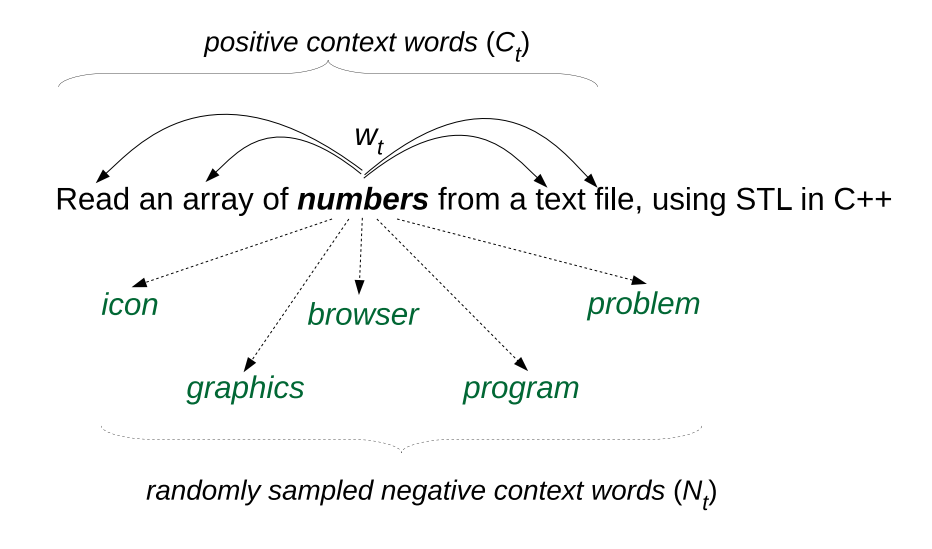
\includegraphics[width=.65\linewidth]{fig/cp5/ye-skip-gram-example}
    \caption{Positive and negative training examples in the Skip-gram model. Figure originally from~\cite{Ye2016} \gm{Unfortunately you can't use this diagram without permission if it is from a published text.}}
    \label{fig:skip-gram-example}
\end{figure}


Using the skip-gram model, one can identify that words $t$ and $s$ are semantically similar 
computing the cosine similarity between their corresponding word embedding representations, i.e., $w_t$ and $w_s$:



\begin{equation}
    cos(w_t,w_s) = \frac{w_t^Tw_s}{\|w_t\| \|w_s\|}
    \label{eq:word-sim}
\end{equation}




% Overview of state-of-the-art model
\medskip
\begin{hangparas}{.0in}{0}
     \textit{BERT model.} Context in the Skip-gram model refers to the positive/negative examples used during the model's training procedures; this, however, does not allow the model to disambiguate words based on their surrounding text. In other words, a Skip-gram model will have a single vector representation for the word \textit{company} even when it can have different meanings, i.e., a business organization or being with someone. In contrast, state-of-the-art models, such as \textit{BERT}~\cite{Devlin2018Bert}, provide different representations for the same word based on the sentence in which a word appears.
    This additional layer allows for more complex operations, such as word disambiguation \red{ref}.
\end{hangparas}



BERT also addresses tasks that need to understand relationships between sentences, which is a task not directly captured by language modeling~\cite{Devlin2018Bert}. \gm{I am struggling with the
idea that tasks 'need' to understand relationships between sentences. More explanation is likely needed.}
To capture sentence relationships, BERT training procedures consider both next word prediction---as in any language model---and also next sentence prediction, i.e., given a pair of sentences $A$ and $B$, the model 
is trained to predict the likelihood that sentence $B$ succeeds (or not) sentence $A$ (Figure~\ref{fig:BERT}). 


\begin{figure}
    \centering
    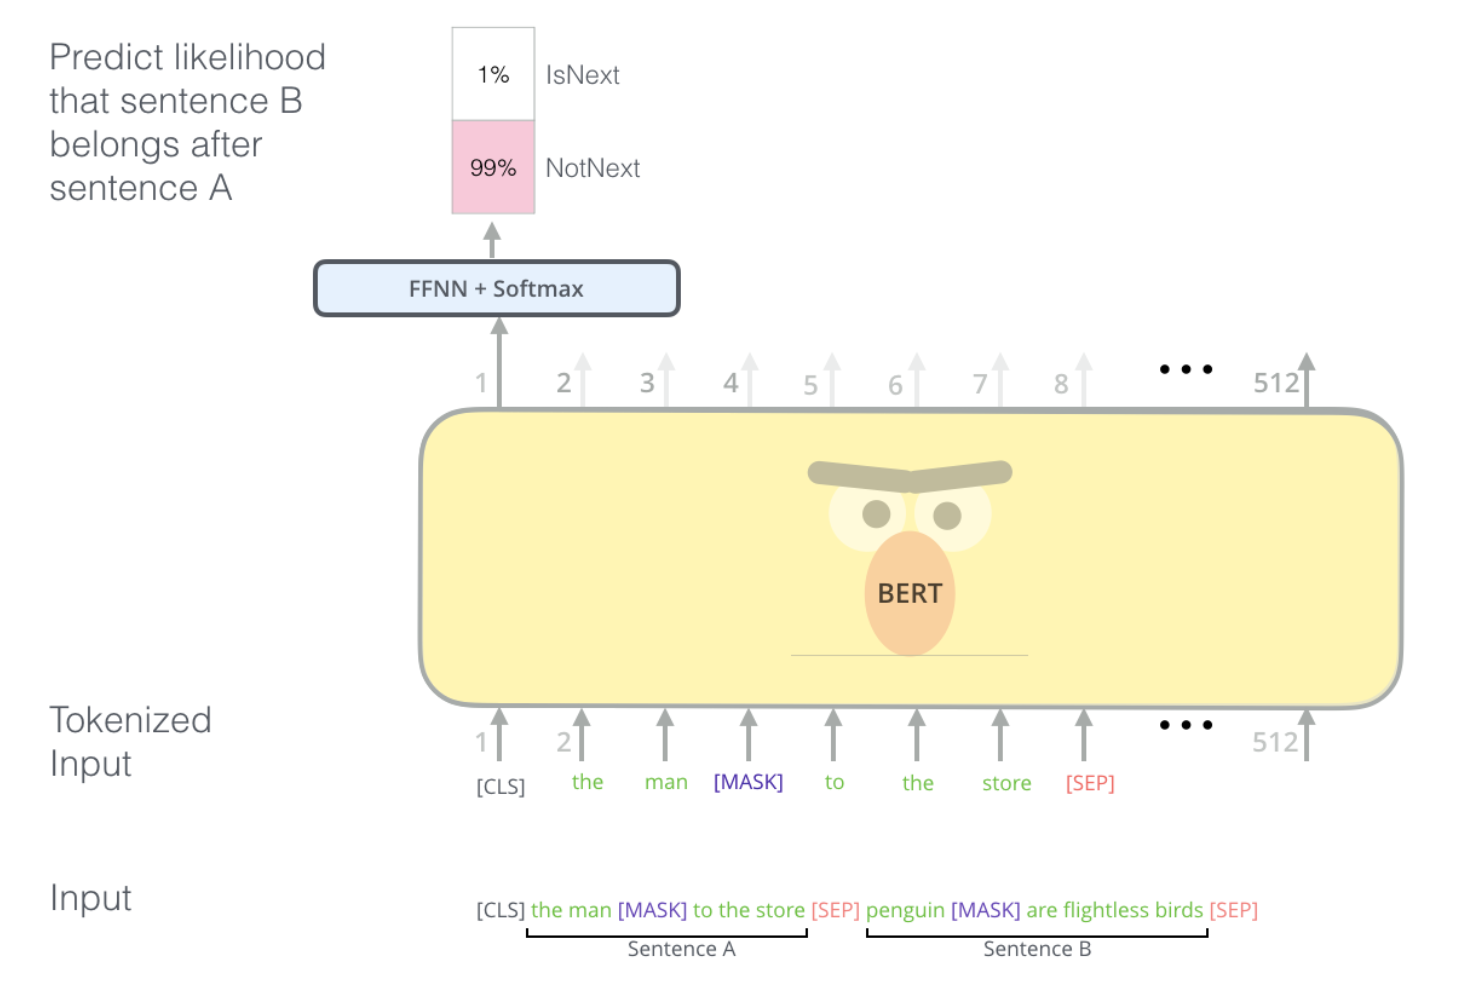
\includegraphics[width=.75\linewidth]{fig/cp5/BERT}
    \caption{BERT next sentence prediction training procedures. Figure originally from~\cite{jay-alammar-bert} \gm{Same issue
    with re-using Figure}}
    \label{fig:BERT}
\end{figure}



Since BERT addresses both next word prediction and next sentence prediction, the model can be used for several
word semantics and sentence relationship tasks such as  ours, i.e., determine the relevance of a sentence within an artifact based on a second sentence representing a task description. \gm{How is
this sentence prediction? Is there precendence for using
BERT on two different artifacts (i.e., the task description
can be considered an artifact or document.)}


% ------------------------------------------------


\subsubsection{Semantic Similarity}
\label{cp5:skip-gram}

\gm{Is this still part of background? There needs to be
some more walking the reader through where this part is
going. Maybe introduction some nomenclature for
actual approaches you are introducing. Let's discuss.}

Similar to lexical similarity,  we investigate if the sentences with the highest semantical similarity are most likely to contain information relevant to the input task.


To compute the semantic similarity between the sentences within a pertinent artifact and a task,
we use the Skip-gram model~\cite{Mikolov2013} with word embeddings specifically trained for the software engineering domain~\cite{Efstathiou2018}.
Since word embeddings provide vector representations at the word level, we follow Conneau et al.'s guidelines~\cite{conneau2018} 
and compute vector representations for an entire sentence by averaging the sum of the word embeddings in that sentence.


Provided that we have embeddings $w_t$ and $w_s$ for the text 
of an input task and an arbitrary artifact sentence, 
their semantic similarity can also be obtained 
using the cosine similarity. In turn, we can select the top-n sentences
with the highest semantical similarity as the ones likely relevant to an input software task.


% ------------------------------------------------


\subsubsection{Artifact-Task Sentence Relationships}
\label{cp5:bert}


We use the BERT model~\cite{Devlin2018Bert} to establish relationships between artifact and task sentences pairs and determine 
the sentences within an artifact that most likely contain information relevant to the task.


Since BERT requires training procedures, we start with an already pre-trained model, namely BERT\textsubscript{uncased}, and we tune it to  identifying task-relevant text.
\gm{Is BERT\textsubscript{uncased} something from elsewhere?}
As done by several other studies (e.g., ~\cite{Chaparro2017, fucci2019, Petrosyan2015}), we use standard cross-validation techniques to ensure  that no data used for evaluation is also used
during the model's training procedures. More specifically, we use 10-fold cross-validation with 70\%, 20\% and 10\% splits for training, validation and testing. 


The model outputs probability scores indicating the likelihood of a sentence being relevant to an input task.
We select the top-n sentences predicted by the model as relevant.



% ------------------------------------------------


\subsection{Frame Semantics}


\art{I still need to check frames based on the tasks in \acs{DS-synthetic}, so there might be updates to this section. }


Given our analysis of relevant sentences in the \acs{DS-synthetic} corpus, we pose that 
sentences with certain meanings, such as the ones that provide instructions on using an entity to achieve some goal,
are sentences that a developer would first pay attention to when inspecting a software artifact and thus, they are more likely to contain task-relevant information. \gm{Will need more on why
this hypothesis.}



We implement this hypothesis as a post-filtering step~\cite{Manning2009IR} applied to the lexical similarity and word semantics approaches.
Given a set of sentences returned by an approach, 
we use the \textit{SEFrame} tool~\cite{marques2021} as a proxy to the sentence's meaning,
checking if the semantic frames obtained by the tool appear in a set of frames drawn from  sentences annotated as relevant in the \acs{DS-synthetic} corpus.





% ------------------------------------------------


\subsection{Approaches Summary}


Table~\ref{tbl:approaches-summary} bundles the approaches that we explore.
The table provides a short identifier for each approach, identifies the research topic that serve as a basis for each approach and provides a short description for them. From now on, we refer to each approach according to their short identifier.

\gm{Isn't there multiple SEframes approaches?}


\begin{table}[H]
\centering    
\begin{scriptsize}
\begin{threeparttable}
\rowcolors{2}{}{lightgray}    
\begin{tabular}{lll}

% \hline

% \multicolumn{2}{c}{\textit{No lock screen controls ever}}  \\



\textbf{Identifier} & \textbf{Based on} & \textbf{Description} \\

\hline


\texttt{baseline} & 
\parbox[l][1cm][c] {1.5cm}{lexical\\similarity} &
\parbox[l][1cm][c] {8.5cm}{
    Uses VSM to identify the top-n sentences most lexically similar to a task description as task-relevant
}
\\


\texttt{word2vec} & 
\parbox[l][1cm][c] {1.5cm}{word\\semantics} &
\parbox[l][1cm][c] {8.5cm}{
    Uses the Skip-gram model to identify the top-n sentences most semantically similar to a task description as task-relevant
}
\\

\texttt{BERT} & 
\parbox[l][1cm][c] {1.5cm}{word\\semantics} &
\parbox[l][1.4cm][c] {8.5cm}{
    Uses BERT to establish relationships between a task description and sentences within an artifact, selecting the top-n sentences 
    that the model predicts as task-relevant
}
\\


\texttt{frame-meaning} & 
\parbox[l][1cm][c] {1.5cm}{frame\\semantics} &
\parbox[l][1cm][c] {8.5cm}{
    \red{TODO}
}
\\


\texttt{frame-matching} & 
\parbox[l][1cm][c] {1.5cm}{frame\\semantics} &
\parbox[l][1cm][c] {8.5cm}{
    \red{TODO}
}
\\



\hline


\end{tabular}
\end{threeparttable}
\end{scriptsize}
\caption{Summary of approaches used to automatically identify task-relevant text}
\label{tbl:approaches-summary}
\end{table}


% \clearpage

\section{Evaluation}
\label{cp5:evaluation}



The goal of our evaluation is to assist the design of tools that use the explored techniques to help developers in locating text relevant to their task. 
To evaluate and compare the techniques,
we report \textit{precision} and \textit{recall} metrics~\cite{manning2010IR} measuring what portion of the \acs{DS-android} text identified by human annotators the techniques automatically identify.
In this context, we believe recall to be the most important metric since failure to identify text that is relevant to a task means that a developer will have an incomplete or partial view of the information needed,
what can lead to faults~\cite{Murphy2005}.
Experimental procedures are as follows.



\subsubsection{Baseline}


As done by~\cite{Lin2021} and~\cite{Ye2016}, we use a standard \texttt{VSM} lexical similarity approach as a baseline. Our rationale to use 
lexical similarity as a baseline is based on the fact that 
both our qualitative analysis (\red{Chapter~\ref{aaa}}) and
related work~\cite{Ko2006a, Freund2015} have shown that developers often use keyword-matching as a first search strategy to locate text that might contain information relevant to their tasks.


Analogous to the semantic similarity-based technique (Section~\ref{cp5:approach-w2v}), the baseline technique uses VSM to compute lexical similarity scores. The baseline outputs the top-n sentences with the highest similarity as the ones likely relevant to an input software task.




\subsubsection{Setup}



We configure each technique to identify a target number of 10 relevant sentences per input task-artifact.
This decision is based on the fact that no more than 20\% of the content of any artifact in the corpora is deemed relevant to a task, which, on average, accounts for 8.93 sentences (\red{Chapter~\ref{}}).
Researchers have also used the same target number of 10 sentences when evaluating techniques  (e.g.,~\cite{Xu2017} or~\cite{Lotufo2012}) able to identify relevant text for certain kinds of artifacts what will also facilitate comparing our results to related work.


\subsubsection{Training Data}


In addition to configuring the techniques' output, two of our techniques use part of the  \acs{DS-android} data for fine-tuning purposes (\texttt{BERT}) and to derive sentence-task frame pairs (\texttt{frame-associations}).
We ensure that no data used to evaluate these techniques is also used in their setup by 
splitting the dataset using standard cross-validation techniques.
We split the dataset into 10 folds, each containing 5 tasks used for evaluation purposes. 
We use the remaining 45 tasks to mine sentence-task frame pairs and to train BERT. 
For BERT, we further split the training data and use 10\% of it to validate the model~\cite{Chaparro2017, fucci2019, Petrosyan2015}.
We refer to this setup of BERT as \texttt{BERT\textsubscript{DS-android}}.


To study the impacts of training data on BERT, we also train the model in a smaller dataset containing six tasks and a total of 1874 sentences, from which 602 of them were deemed relevant by 20 participants with software development experience (\red{Chapter~\ref{aaa}}). Due to the synthetic nature of the tasks in this dataset, we refer to this 
second configuration as \texttt{BERT\textsubscript{DS-synthetic}}.




\subsubsection{Metrics}


We compute values for \textit{precision} and \textit{recall} metrics based on the golden labels available in the \acs{DS-android} corpus and sentences deemed relevant to a task by at least two human annotators.
For a detailed definition of each metric, we refer to the evaluation outcomes in Table~\ref{tbl:type-I-II-errors}, where  columns represent  labels provided by the annotators and rows,
the text identified as relevant or not by a technique.

% 

\medskip
\begin{table}[H]
\centering    
\begin{scriptsize}
\begin{threeparttable}
\begin{tabular}{l|l|l}

\hline

\textbf{}
& \textbf{Relevant}    
& \textbf{Not-relevant} \\

\hline

\textbf{Identified as relevant} & true positive ($TP$) & false positive ($FP$) \\
\hline
\textbf{Identified as Not-relevant} & false negative ($FN$) & true negative ($TN$) \\
\hline

\end{tabular}
\end{threeparttable}
\end{scriptsize}
\caption{Evaluation outcomes}
\label{tbl:type-I-II-errors}
\end{table}

    



\paragraph{\textbf{Precision}}

Precision measures the fraction of the sentences identified that are relevant over the total number of target sentences identified, as shown in Equation~\ref{eq:cp5:precision}.



\begin{equation}
\label{eq:cp5:precision}    
    Precision = \frac{TP}{TP + FP}
\end{equation}



\paragraph{\textbf{Recall}} Recall represents how many of all the annotated sentences are identified by a technique (Equation~\ref{eq:cp5:recall}).


\begin{equation}
\label{eq:cp5:recall}        
    Recall = \frac{TP}{TP + FN}
\end{equation}



\medskip
Precision means identifying only text that is relevant, whereas recall means identifying all relevant text.
Ideally, we would aim for a technique with high precision and recall. Unfortunately, this is often not possible and we must reach a compromise.
Based on studies that have observed that developers face more challenges finding information related to their task~\cite{Robillard2015, Maalej2013}, we argue that in the bound number of sentences outputted by a technique, developers can quickly discard what they judge that is not relevant. Hence, we aim to find as much of the relevant text within a technique's output, thus the reason why we favour recall.







\subsection{Results}


Table~\ref{tbl:techniques-results-overall} shows evaluation results. 
In the table, rows provide details about a specific technique while columns discriminate 
precision and recall values and which filters were applied. 
When interpreting the results, it is worth noting that achieving high accuracy in \acs{DS-android} is challenging
due to the fraction of sentences deemed relevant, which comprises 20\% of the entire data.
For example, API documents in the corpus have an average of 109.22 sentences per document, from which 9.62 sentences are relevant. 
This means that, with a target number of 10 sentences identified per technique, a $1.0$ recall is only possible when a technique identifies the exact 10 sentences that are relevant for this kind of artifact.



\begin{table}[H]
\centering    
\begin{small}
\begin{threeparttable}
\begin{tabular}{lccccc}


\textbf{technique} & 
\textbf{precision} & \textbf{recall} & 
$\Delta$ \textbf{precision} & $\Delta$ \textbf{recall} \\


\hline


\texttt{baseline} &
0.30 & 0.33 &  
0.38 & 0.48 
\\

\texttt{word2vec + association-pairs} &
0.52 & 0.53 &  
0.52 & 0.51
\\

% \texttt{BERT\textsubscript{DS-synthetic}} &
% 0.54 & 0.55 & 0.51 & 
% 0.55 & 0.57 
% \\

\texttt{BERT\textsubscript{DS-android} + frame-elements} &
0.55 & 0.56 & 
0.55 & 0.56 
\\

\hline

\end{tabular}
\end{threeparttable}
\end{small}
\caption{Pyramid precision, pyramid recall comparison}
\label{tbl:approach-results-overall}
\end{table}





The \texttt{baseline} technique, which uses VSM, achieves precision and recall scores of $0.30$ and $0.33$, respectively. 
Although this result is not surprising, it corroborates results from related literature showing limitations of lexicon-based approaches, as detailed in Section~\ref{cp5:background}.





Using \texttt{word2vec}, precision and recall scores increase to $0.46$ and $0.45$. We also observe that applying sentence-semantic filters to \texttt{word2vec}'s output further improves precision and recall values. Notably, the 
\texttt{frame-associations} filter achieves up to $0.52$ recall. These results suggest that both word semantics and sentence
semantics shorten lexical gaps when identifying information relevant to a software task.


Recall values for 
\texttt{BERT} range from $0.57$ to $0.60$ for 
the \texttt{DS-synthetic} and the \texttt{DS-android} configurations.
Sentence semantic filters do not provide substantial changes for \texttt{BERT}, where \texttt{frame-associations} yields $0.61$ recall. 
We believe that the 
lack of differences between the two \texttt{BERT} models are explained by 
the fact that the model uses \textit{transfer learning} and thus, the  
large corpora used to train the model before fine-tuning assists prediction steps even for tasks and artifacts that the model was not trained on. In turn, the lack of improvements when applying semantic filters might relate to how the model's \textit{attention mechanism} may already correlate the text in a task and an artifact (Section~\ref{cp5:bert}).




% \section{Summary}
\label{cp5:summary}



In this chapter, we introduced six semantic-based techniques 
that incorporate semantics of words and sentences
to identify task-relevant text across a range of natural language artifacts.
We compare our proposed techniques to a state-of-the-art technique, AnswerBot,
specific to Stack Overflow artifacts and 
we evaluate them using a dataset that comprises  50 software tasks about Android development for
which human annotators identified pertinent text per task across a variety of kinds of software
artifacts.
Evaluation results show that semantic-based techniques 
achieve recall comparable to AnswerBot, but without the need for artifact-specific data, 
and that some of our proposed techniques perform equivalently well across
multiple artifact types. 



% \setcounter{chapter}{5}
\setcounter{rq}{1}


\chapter{Evaluating Text Automatically Identified}
\label{ch:assisting}



In a previous chapter, we have shown that semantic-based techniques can identify part of the text 
that human annotators deemed relevant to a number of artifacts associated with Android tasks.
This, however, does not address whether the text automatically identified assists a software developer
 in completing her task.



To shorten this gap, this chapter presents a \textit{controlled experiment} 
where we evaluate how developers complete software tasks when assisted, or not, by a tool that 
embeds one of our semantic-based techniques. 
We use three software tasks related to well-known Python modules and
we report qualitative and quantitative results from \red{12} participants with software development background who attempted these tasks. 



We start by describing experimental procedures (Section~\ref{cp6:procedures}) and then by presenting the results of our experiment (Section~\ref{cp6:results}). Section~\ref{cp6:summary} summarizes our key findings.



\clearpage

\section{Experimental Setup}
\label{cp6:procedures}



\gm{You need to provide the overall
design first. Hard to understand why
the tasks are as they are. More "Design' up-front.}


To determine how a tool embedding a semantic-based technique might assist developers complete a software task, we question whether:



\begin{enumerate}
    \item \textit{a developer would produce a more correct solution when assisted by such a tool;}
    \item \textit{the text automatically identified by the tool as potentially relevant to a task in a software artifact pertinent to that task is similar to text that developers would deem relevant; and if}
    \item \textit{a developer finds that the text automatically identified by the tool in an artifact under inspection assists her towards task completion.}
\end{enumerate}



To investigate these questions, we designed an experiment where participants attempted two programming
 using (or not) a tool that applies the \texttt{BERT} technique (Section~\ref{cp5:approach-bert})
 to  identify task-relevant text in the artifacts that were available to a participant in each task---highlighting the text automatically identified by the semantic-based technique in these artifacts. 


For each task, we compare solutions  submitted by participants who did, or did not, use the tool to assist them in that task. 
For that, we run a set of test cases that evaluate the correctness of the submitted solutions, what helps us answer RQ1.


In the tasks that participants performed without tool support, we asked them to manually indicate in the artifacts available for that task the text that they deemed useful for that task.
We use the manually provided text to investigate RQ2, analyzing to which extent our tool identifies the same text for that task.


We also asked participants to indicate how useful were the highlights shown in each of the artifacts available in the tool-assisted task
and prompted them to provide any additional feedback that they wished to share about the tool or the experiment (RQ3).






We detail experimental procedures in the following subsections.






% Our experiment's main hypothesis is that:


% \medskip
% \begin{bluequote}
%     \textit{text automatically identified by a semantic-based technique assists a 
%     developer complete her software development task.} 
% \end{bluequote}



% To test this hypothesis, 
 
%  \gm{Setting this up as a test of
%  a hypothesis sets a high bar where
%  there will be expectations of
%  refuting a null hypothesis. Is that
%  where you want to go?}

% %  For each of these tasks, we provided to the participants a curated list of natural language artifacts related to the task
% % and we asked them to code a solution for the task.
 
 
% %  when assisted (or not) by a
% %  tool that embeds one of the semantic-based techniques that we have explored previously ({Section~\ref{cp5:results-all}). 

% \gm{You need to provide the overall
% design first. Hard to understand why
% the tasks are as they are. More "Design' up-front.}

% In a first task, a participant manually identifies text relevant to that task (while performing the task)
% in a set of curated artifacts containing information that could assist the participant complete the task at hand.
% With this first task, we evaluate how the text that a participant manually identified as relevant
% compares to the text that an automatic technique would identify for that same task. 



% In a second task, each artifact associated to the task has a set of highlighted sentences. These 
% sentences represent text that an automatic approach ({Section~\ref{cp5:results-all}) identified as potentially useful for that task. 
% We ask a participant to indicate whether the highlights shown helped her complete their task.
% Hence, with this second task, we evaluate what is the participants' perceived usefulness of the text automatically identified.





% % \art{Add a figure to help summarizing the experimental setup?}



% \art{say somewhere that the experiment was performed remotely and without the researcher's assistance. }


\subsection{Design}


The experiment's independent variable represents the task configuration, i.e., if a participant had to manually indicated what text they deemed relevant to a task
or if our tool automatically did this step. We refer to these two configurations as \textit{manual} or \textit{tool-assisted}. 


Based on our independent variable, we follow a \textit{within-subjects} design. Each participant is exposed to exactly one manual task and one tool-assisted task.
We assigned tasks to a participant randomly. Nonetheless,  
we ensured that each task configuration (manual or tool-assisted) was seen by an equal number participants.
\gm{how is this design within-subjects?
Aren't you comparing across
the tasks which means across subjects?}








\subsection{Tasks}
\label{sec:experiment-tasks}



We expect the experiment to be executed offline, i.e., the experiment has self-contained instructions that allow a participant to perform their assigned tasks without any supervision.
\gm{Why not just say the participants
completed the tasks on their own time?}
This requires tasks that are easy to understand and perform in a single experimental session. At the same time, our main hypothesis requires tasks for which a developer will likely benefit from the use of additional information to complete.


These criteria lead us to select Python w3resource tasks\footnote{\url{https://www.w3resource.com/python-exercises/}}
that required usage of at least one module external to the Python core modules~\cite{thiselton2019}.
By using an external module, we aim to reduce the likelihood that a participant 
can provide a solution for a task without consulting any of the artifacts accompanying that task. 






Table~\ref{tbl:python-tasks-modules} details the tasks that we have selected. 
We chose these tasks due to how they focus on modules widely adopted both by open source systems and by private companies.
For example, the \texttt{NYTimes} task involves using a HTML parser, namely \texttt{BeautifulSoup},
which Reddit---a social news aggregator with approximately 430 million monthly users---uses 
to parse urls and identify images shown on its posts' headlines~\cite{bs4-reddit}. 
Similarly, the \texttt{Titanic} task encompasses using \texttt{Pandas}, a data analysis and manipulation module
used in many open source data science projects~\cite{ma2017, shrestha2020}.





\begin{table}
\centering
\caption{Python tasks}
\begin{footnotesize}
\rowcolors{2}{}{lightgray}
\begin{tabular}{ll}
\hline
\textbf{Task} & \textbf{Description}                                                                                         \\
\hline
\hline
%
\parbox[l][1cm][c]{1cm}{Practice task}       &
\parbox[l][1cm][c]{11cm}{Given three dictionaries representing address books,
you must write an algorithm using the Python core \texttt{dict} module to merge them.}    \\
\hline
%
Distances     &
\parbox[l][1.3cm][c]{11cm}{Given a string representing a rendezvou point and a list of suggested picnic addresses
    you must write an algorithm using the \texttt{geopy} module to find the  picnic address closest to the rendezvou point.} \\
%
NYTimes       &
\parbox[l][1cm][c]{11cm}{Given a string representing the url for NY Times Today's,
    write an algorithm using the \texttt{BeautifulSoup} and \texttt{requests} modules to scrape all the headlines of that page.}
\\
%
Titanic       &
\parbox[l][1cm][c]{11cm}{Given a string representing a url for the titanic dataset,
    you must write an algorithm using the \texttt{pandas} and \texttt{seaborn} modules to create a barchart of the data.}    \\
    
\hline
\end{tabular}
\end{footnotesize}
% \smallskip
\label{tbl:python-tasks-modules}
\end{table}









\subsection{Artifacts}
\label{sec:experiment-artifacts}


Each task requires a set of artifacts that a participant could peruse for information that could assist them complete the task.
We select artifacts for a task following procedures similar to the ones we used to create the \acs{DS-android} dataset (Chapter~\ref{ch:android-corpus}). 
For each of the tasks in Table~\ref{tbl:python-tasks-modules}, we use the Google search engine to obtain up to ten artifacts that likely contain relevant
information for that task. 






\subsection{Participants}



We advertised our study to both developers in our professional network and to computer science students at the several universities. 
This provides for breadth of experience where both novice and expert developers attempt the tasks in our experiment. 


With regards to computer science students, we sent the study only to third and fourth-year students to ensure that they had the necessary background required to perform the study's taks.
At this point in the curriculum, students should be familiar with Python and they should be able to come up with a solution 
for a software task when provided with artifacts containing information for that task.


To compensate participants for their time, we offered them the opportunity to enter a raffle for one of two iPads 64 GB.






\subsection{Procedures}
\label{cp6:evaluation-procedures}



The experiment was completely offline, i.e., it could be performed at a participant's personal computer
without the presence of one of the researchers. Each participant had to complete a practice task---separated from the experimental tasks---and two tasks (manual and tool-assisted) drawn from the tasks in Table~\ref{tbl:python-tasks-modules}. 


Each experimental session lasted no more than two hours; this length of time was selected based on two pilot sessions. 
Feedback from these pilots also helped to refine the experiment's instructions, where we included a short video showing how to install the web browser plugin and how to use Colab, the online environment where participants performed each task (Section~\ref{cp6:environment}).






We began each session gathering consent and requesting participants to install a web browser plugin which we used to gather data.
Setup was followed by a short tutorial explaining the experiment and describing how to use the plugin and Colab. 
The practice task allowed participants to familiarize themselves with the content of a task, the web browser plugin and Colab. 



For each task, including the practice tasks, we asked a participant to write a solution for the task
when provided with a fixed set of artifacts, e.g., official API documentation, Stack Overflow posts, or web tutorials, 
associated with that task.  


In the control task, a participant was instructed to use the web browser plugin to highlight any text that they deemed relevant to the task-at-hand. 
\gm{Do they highlight text as they
work or after the task?}
In the tool assisted task, the plugin automatically highlighted sentences that our semantic-based technique identified as relevant for the task. 
For this second task, we had one extra step asking the participant to rate---using a Likert scale---how helpful were the highlights automatically identified per artifact available. 
\gm{More detail about exactly
what participants were asked to
do and experimental materials
should be published or in Appendix
of thesis.}


We concluded the study by asking participants if they would like to provide any additional information and 
by giving them the opportunity to join the raffle, if so they wished. 



% \subsubsection{Summary of procedures}

% Based on our experimental procedures, we could gather:



% \begin{enumerate}
%     \item a participant's submitted solution (written Python code) for each task;
%     \item a participant's highlights for the control task; 
%     \item a participant's perception on the usefulness of the automatically identified highlights for the tool assisted task, and;
%     \item any additional feedback (written text) that a participant wished to provide us.
% \end{enumerate}




\subsection{Colab}
\label{cp6:environment}


To ensure that participants had the same conditions to perform each task
and also to minimize setup instructions, we used Google Colab\footnote{\url{https://colab.research.google.com/}} as our coding environment. 
% By using Colab, we also expect setup instructions to be minimal 
% so that we allow a participant to focus on the task and experimental procedures.



Figure~\ref{fig:nytimes-task-colab} shows an example of our online environment for the \texttt{NYTimes} task.
At the left-hand side, participants had the task description and examples of input and output scenarios as well as a list of resources associated with that task. 
By clicking on the coding environment link, participants were redirected to Colab (right-hand side),
where they had a code editor with amenities commonly found in modern IDEs, such as code completion and syntax highlighting. 



Through Colab, a participant could compile their solution and test it against the examples shown alongside the task description.
Upon testing, the system would display full details about the test cases, e.g., the test's input, which assertion failed, and why. 




\clearpage

\begin{landscape}
\begin{figure}
    \centering
    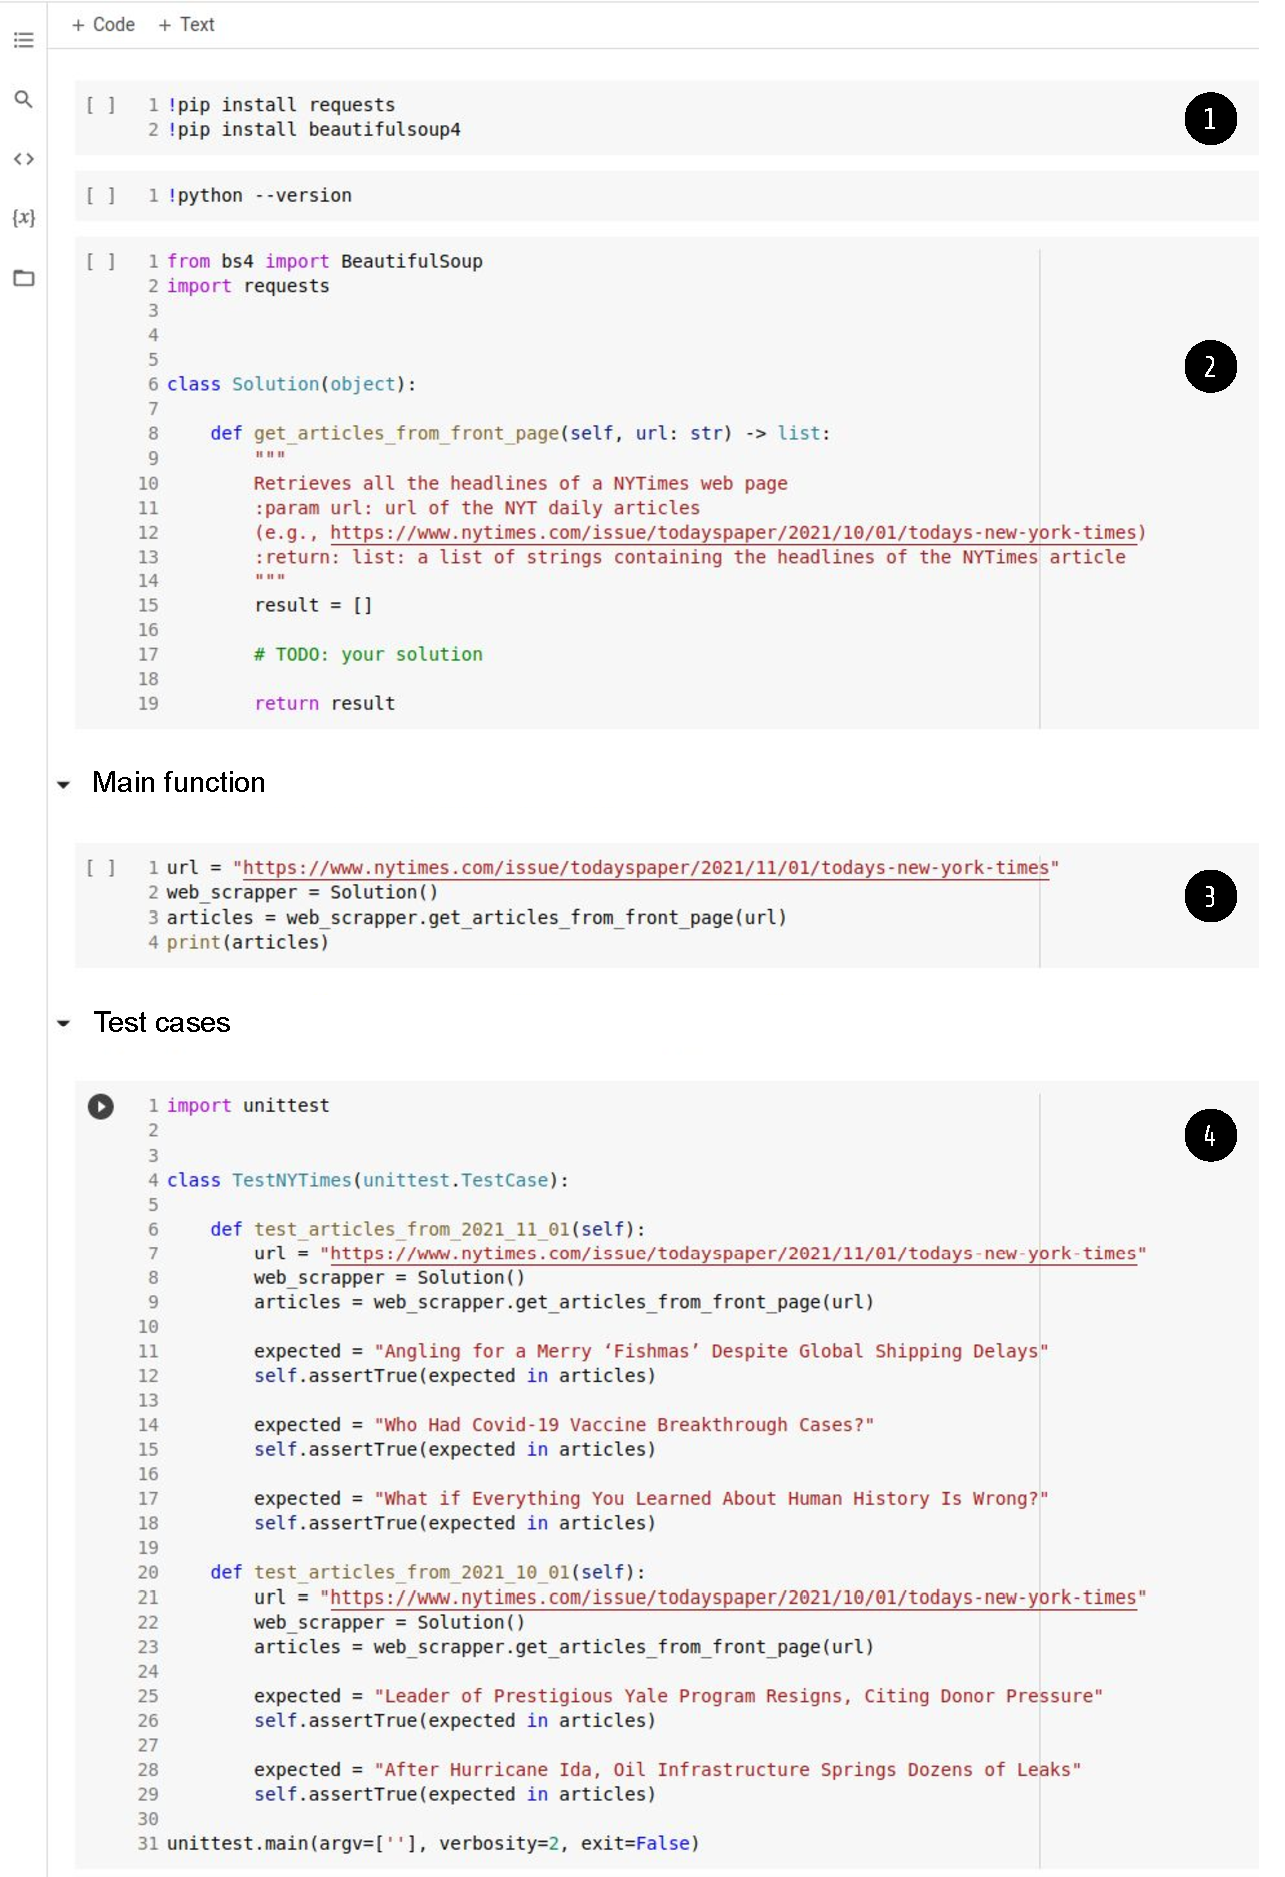
\includegraphics[width=1.5\textwidth]{cp6/task-colab.pdf}
    \caption{NYTimes task and Colab environment.}
    \label{fig:nytimes-task-colab}
\end{figure}
\end{landscape}

\clearpage


\subsection{Analysis}



Table~\ref{tbl:experiment-data} summarizes the data we collected based on experimental procedures.
We use the gathered data to investigate our main hypotheses according to the following metrics.



\begin{table}
\caption{Data collected}
\begin{small}
\vspace{-1mm}  


\begin{threeparttable}    
\rowcolors{2}{}{lightgray}
\begin{tabular}{ll}
\hline    
\textbf{} & \textbf{Data collected}  \\ 
\hline
\hline
1 & 
\parbox[l][0.8cm][c]{11cm}{
    participant's submitted solution (written Python code) for each task
}  
\\
%
2 & 
\parbox[l][0.8cm][c]{11cm}{
     participant's highlights for the control task
}  \\
3 & 
\parbox[l][1cm][c]{11cm}{
    a participant's perception on the usefulness of the automatically identified highlights for the tool assisted task
}  \\
4 & 
\parbox[l][0.8cm][c]{11cm}{
    any additional feedback (written text) that a participant wished to provide us
}  \\
\hline
\end{tabular}
\end{threeparttable}    
\end{small}
\smallskip
\label{tbl:experiment-data}
\end{table}
    



\subsubsection{Submitted Solution}

 
The correctness of a submitted solution is measured by the number of passing test cases
when running that solution against a set of 10 test cases. 
A solution with compile errors has a correctness score of zero.


\smallskip
\begin{small}


\begin{equation}
    Correctness = \frac{ \text{\textit{\# of passing test cases}}}{\text{\textit{\#  of test cases}}}
\end{equation}
\end{small}

% \smallskip
% According to this definition, 


\subsubsection{Manual Highlights}


We compare the participants' manual highlights  against the ones automatically identified by our semantic-based technique. 
For that, we use \textit{precision} and \textit{recall} metrics. 




Precision measures the fraction of the automatically identified text that was  considered relevant
by the participants.

\smallskip
\begin{small}


\begin{equation}
    Precision = \frac{
        \text{\textit{automatic highlights}~} \cap 
        \text{~\textit{manual highlights}}
    }{\text{\textit{automatic highlights}}}
\end{equation}
\end{small}


Recall represents how many of all the manual highlights were identified by the semantic-based technique that we applied.

\smallskip
\begin{small}

\begin{equation}
    Recall = \frac{
        \text{\textit{automatic highlights}~} \cap 
        \text{~\textit{manual highlights}}
    }{\text{\textit{manual highlights}}}
\end{equation}
\end{small}

\medskip
\art{Argue which metric matters the most here}


\art{Discuss how to account for variability in what the participants highlighted}



\subsubsection{Usefullness of the Automatic Highlights}


We use a diverging stacked bar chart~\cite{Heiberger2014} to analyze the  Likert scale
responses on the usefulness of the text automatically identified.


Usefulness indicates the percentage of responses agreeing or disagreeing with whether sentences
automatically highlighted assisted a participant in completing a task.


\smallskip
\begin{small}

\begin{equation}
Usefullness = \frac{
    \text{\textit{\# of responses at i}}
}{
    \text{\textit{total \# of responses}}
}
\end{equation}
        

\begin{equation*}
i \in \{ 
    \text{\textit{
        (strongly) agree, neither agree or disagree, (strongly) disagree
    }}  
\}
\end{equation*}
\end{small}

% This analysis complements the quantitative comparison of manual and automatic highlights.
% By asking participants to reflect on the usefulness of the text automatically identified, 
% we seek to minimize risks related to how a participant might have missed highlighting
% text that assisted them complete a task~\cite{easterbrook2008}.





\subsubsection{Written Feedback}

 
We use qualitative methods to analyze participants' responses to the open-ended questions. 

\art{Think this through...}




\clearpage



\section{Results}
\label{cp6:results}

We organize results assessing the solutions submitted by the participants, 
comparing manual and automatically identified text as well as discussing the usefulness of the highlights shown 
by the study's tool.

\gcm{Seems like the usefulness of highlights is more important than
the comparison.}



\section{Tasks Correctness}
% \section{Does \acs{beskar} lead to more correct solutions?}
\label{cp6:correctness}



When assisted by a tool able to automatically highlight text identified as relevant to a task, we expect that a developer can produce a solution 
that is equally or more correct than the solution of a developer who attempted a task without tool support. 
To explore the correctness of the solutions submitted by participants who attempted a task 
with and without tool support, we compile their code and run it against a set of test cases 
that assess their correctness.


\subsection{Method}


The correctness of a submitted solution is measured by the number of passing test cases
when running that solution against a set of 10 test cases, specific to each task. 
A solution with compile errors has a correctness score of zero.


\smallskip
\begin{small}


\begin{equation}
    Correctness = \frac{ \text{\textit{\# of passing test cases}}}{\text{\textit{\#  of test cases}}}
\end{equation}
\end{small}

\subsection{Results}
 

\subsection{Comparison of manual and automatically identified task-relevant text}
\label{cp6:comparison}


To assist a developer to complete a task correctly, a tool that
automatically identifies text pertinent to that task would ideally 
identify text that humans have also considered as relevant.
\gcm{Why ideally? Maybe humans are terrible at identifying relevant text?}
Procedures from our control task asked participants to identify text they deemed useful. We
 compare this manually provided data against the text automatically identified.



% \paragraph{\textbf{Metrics.}}

\subsubsection{Metrics}

To investigate the overlap between the participants' manual highlights and the 
the automatic highlights identified by the study tool we use \textit{precision}, \textit{recall}~\cite{manning2010IR}, and \textit{pyramid precision}~\cite{Nenkova2004}.
We compute these metrics for each artifact of each task and report their average.


For this analysis, we follow Lotufo et al.'s procedures~\cite{Lotufo2012} and we consider any text marked by any participant as relevant.
We investigate if our tool  automatically identifies text that multiple participants deemed relevant
 via \textit{pyramid precision}. 
Details for each metric are as follows. 

\medskip

Precision measures the fraction of the text automatically identified  that participants deemed relevant (Equation~\ref{eq:precision-cp6}). 

\smallskip
\begin{small}
\begin{equation}
    Precision = \frac{
        \text{\textit{automatic highlights}~} \cap 
        \text{~\textit{manual highlights}}
    }{\text{\textit{automatic highlights}}}
\label{eq:precision-cp6}    
\end{equation}
\end{small}


Recall represents how many of all the manual highlights were identified by the semantic-based technique applied by our tool (Equation~\ref{eq:recall-cp6}). 



\smallskip
\begin{small}
\begin{equation}
    Recall = \frac{
        \text{\textit{automatic highlights}~} \cap 
        \text{~\textit{manual highlights}}
    }{\text{\textit{manual highlights}}}
\label{eq:recall-cp6}    
\end{equation}
\end{small}

\medskip


\textit{Pyramid precision} compares the text automatically identified to an optimal output, i.e., one where---for the same number of sentences---we identify sentences selected by the most number of participants (Equation~\ref{eq:pyramid-precision-cp6}). The more we identify text that more participants indicated as relevant, the higher pyramid precision is.



\smallskip
\begin{small}
\begin{equation}
    \triangle Precision = \frac{
        weight(\text{\textit{automatic highlights}~})
    }{weight(\text{\textit{optimal highlights}})}
\label{eq:pyramid-precision-cp6}    
\end{equation}
\end{small}
    


To illustrate these metrics, consider an artifact with 4 sentences $\{s_1, s_2, s_3, s_4\}$ that have been selected by $\{2, 0, 1, 1\}$ participants, respectively.
% For an output identifying two sentences for this artifact, an optimal solution would identify sentences $\{s_1, s_3\}$. 
Table~\ref{tbl:metrics-example} shows precision, pyramid precision, and recall metrics in a scenario where we output sentences $\{s_2, s_3\}$ as relevant.
    


\input{sections/cp6/tbl-metrics-example}


% Note that pyramid precision is equal or lower than precision. For example, $Precision(s_1, s_3) = Precision(s_3, s_4) = 1.0$, but 
% results for pyramid precision differ, i.e., 
% $\triangle Precision(s_1, s_3) = 1.0$ and $\triangle Precision(s_3, s_4) = 0.66$. This allows us to check if our tool 
% identified the text deemed relevant by most of the participants who inspected an artifact.



% \paragraph{\textbf{Data.}}
\subsubsection{Data}

Participants who indicated what text was relevant to their assigned control task produced a total of 415 highlights with an average of 7 highlights (std $\pm 3$) per artifact inspected.
On average, this comprises 9\% of the entire content of the artifacts in our experiment. 


Some participants also selected code snippets as relevant to a task---a threat that we discuss in Section~\ref{cp6:threats}. 
Code snippets account for 30\% of the highlights produced, but we remove them from our analysis since our semantic-based approach 
operates on text only. For the textual highlights,
Krippendorf's alpha indicates good agreement of what text in an artifact participants deemed relevant ($\alpha = 0.68$)~\cite{Krippendorff1980, passonneau2006}.
We compare these manually produced highlights to the text automatically identified by our tool.



% \subsubsection{Results}


% \paragraph{\textbf{Results.}}
\subsubsection{Results}



Table~\ref{tbl:comparison-task-wise} summarizes the average of precision, pyramid precision, and recall metrics for each of the tasks in the experiment.
Precision scores range from 0.55 to 0.68, while pyramid precision scores range from 0.55 to 0.57, which suggests that our tool failed to identify some of the text that participants deemed the most relevant.



The results in Table~\ref{tbl:comparison-task-wise} corroborate 
the correctness scores detailed in Figure~\ref{fig:correctness-by-task}. For example, 
in the \texttt{distances} task, participants who performed the task with tool support had solutions less correct than participants in the control group.
This was the task with the lowest precision, recall and pyramid precision values. 
In contrast, the task where participants assisted by our tool obtained the best correctness scores, namely \texttt{titanic}, is the one with the best precision, recall and pyramid precision values.





\input{sections/cp6/tbl-comparison-overall}



Table~\ref{tbl:comparison-artifact-type-wise} details evaluation metrics artifact-type wise. 
Stack Overflow posts and API documentation have the highest precision scores. For these types of artifacts, pyramid precision indicates that the 
text automatically identified on Stack Overflow was the text that several participants deemed relevant. 
The same does not apply to API documentation, i.e., our tool failed to detect a portion of the text that many participants deemed relevant. 
Miscellaneous web pages were the artifact type with the lowest scores. As we detail in Section~\ref{cp6:usefulness},
participants indicated that the text identified for this type of artifact was the least useful.



\input{sections/cp6/tbl-comparison-per-artifact-type}


\gcm{And how does this compare to Chapter 5 results?}

\art{add comparison. }






% \section{Is \acs{beskar} useful?}
\section{Result: Usefulness Analysis}
\label{cp6:usefulness}




% caused by individual differences between the participants who performed a task with and without tool support, what can justify a similar level of correctness in the results; or the presence (or lack) of overlap between the manual and automatically identified 
% text. 
% However, this does not imply that the tool helped participants accomplish their task. 


To further explore if the highlights shown by the tool were helpful, we also asked a participant 
to indicate whether the highlights assisted them complete their assigned task. 
In this section, we described results for this analysis. 



\subsection{Method}



\subsection{Results}



% We use a diverging stacked bar chart~\cite{Heiberger2014} to analyze the  Likert scale
% responses on the usefulness of the text automatically identified.


% Usefulness indicates the percentage of responses agreeing or disagreeing with whether sentences
% automatically highlighted assisted a participant in completing a task.


% \smallskip
% \begin{small}

% \begin{equation}
% Usefulness = \frac{
%     \text{\textit{\# of responses at i}}
% }{
%     \text{\textit{total \# of responses}}
% }
% \end{equation}
        

% \begin{equation*}
% i \in \{ 
%     \text{\textit{
%         (strongly) agree, neither agree or disagree, (strongly) disagree
%     }}  
% \}
% \end{equation*}
% \end{small}





% \subsubsection{Written Feedback}

 
% We use qualitative methods to analyze participants' responses to the open-ended questions. 

% \art{Think this through...}



\subsection{Summary of results}


Results from our experiment suggest that
participants find the text automatically identified
most useful when the semantic based technique applied by our tool 
identifies text that humans deemed relevant to a task.
In such scenario, we observe that participants 
produced more correct solutions. 
However, when it failed to detect the text deemed relevant,
participants found the tool's output not as useful and 
their solutions had more errors. 
These results suggests that our tool might positively or negatively 
impact how a developer completes a task. 



\subsection{Threats to Validity}
\label{cp6:threats}




Our experiment compares solutions submitted by participants who attempted each task with and without tool support. 
This represents a between groups design~\cite{Lazar2017-cp3} and we discuss threats inherent to it. 



Since we compare results from different participants, our analysis might be subject to substantial 
impact from individual differences~\cite{Lazar2017-cp3}. 
For example, participants who performed a task with tool support may have been more experienced than participants 
who did the same task without tool support what affects correctness scores.
As another example,  participants' skill and background 
influences the text that they indicate as relevant in the control task as well 
what text they perceive as useful in the tool-assisted task. 
We minimized these threats by recruiting participants of varied background and randomly
assigning tasks to each participant.



The tasks in our experiment impact generalizability. 
Although we opted for simple tasks, we ensured they 
modules used in our tasks were representative. 
For example, we found open-source systems\footnote{\url{https://github.com/ArchiveBox/ArchiveBox/issues/18}} using \texttt{BeautifulSoup} 
with function calls similar to the ones needed to complete the \texttt{NYTimes} task.
Nonetheless, there are clear differences in the artifacts one can gather 
based on the domain or programming language of a task~\cite{baltes2020}.
Hence, we consider other domains and a wider range of task 
and artifacts for future work. 



The selection of tasks also affects our conclusions. We opted for Python programming tasks that 
required writing code, which we use to assess correctness. 
As observed by other researchers~\cite{satterfield2020, meyer2020}, developers
work on many different tasks, some of which focus on code~\cite{Meyer2017}
while others on information seeking~\cite{gonccalves2011}, e.g., finding duplicated bug reports or researching visualization libraries to identify the most suitable one~\cite{satterfield2020}.
Had we decided to use information-seeking tasks, participants could have produced a different set of highlights,
perhaps selecting fewer code snippets. 
Given that 
our experiment was completely remote, instructing participants on how to perform information-seeking 
tasks would have been more difficult. Furthermore, objectively judging their correctness 
would also be more strenuous, which would lead to a different experiment with challenges and risks of its own.




The fact that we consider the text marked by any participant as relevant 
also affect our conclusions. 
We refrain from excluding text selected by a few participants from our analysis 
for reasons similar to the ones in our characterization of task-relevant information (Chapter~\ref{ch:characterizing}). That is, the text marked by these participants may still contain valuable information. 
We minimize this threat by reporting both precision and pyramid precision, where we observe that 
our approach failed to detect the text that multiple participants deemed relevant
for some tasks or types of artifacts. 



Concerning the text automatically identified by our tool, we gather usefulness at the artifact level.
Suppose we had gathered usefulness at the sentence level. In that case, we could have used this information 
to further refine our analysis, for example, reporting precision and recall 
at different usefulness levels or computing accuracy based on the participants' input, as done by Xu et al~\cite{Xu2017}. 
However, asking participants to provide feedback at the sentence level would have considerably increased the time we estimated that the experiment would take,
which would impact recruitment. We weighed the benefits and drawbacks of a fine-grained or more coarse-grained 
analysis, and we opted for the latter so that this would not be a barrier to people deciding on 
whether to participate in our experiment.
\section{Summary}
\label{cp6:summary}


% \art{ask about summary and better way to position conclusions from the experiment}

In this chapter, we presented an experiment to evaluate whether \acs{tool},
 a tool that embeds a semantic-based technique, assists a developer working on a software task. 
The experiment examined how 24 participants with software development backgrounds attempted 
two programming tasks with or without such a tool. 
Results from this experiment indicate that, 
participants found the text automatically identified and shown by our tool useful in two 
out of the three types of artifacts that assisted them completing their assigned tasks,
where our automatic approach identified on average 58\% of the text that participants deemed relevant. 
These results encourage further exploration of semantic-based techniques, 
embedding them into tools that ultimately facilitate a developer's work.


% \setcounter{chapter}{6}


\chapter{Discussion and Future Work}
\label{ch:discussion}

\gcm{In conducting the studies reported on in
this dissertation and in developing the
techniques explored, we made many decisions.
In this chapter, we discuss the limitations
and trade-offs that resulted and discuss
future avenues for exploration.}

%In this chapter, we discuss questions
%and decisions not addressed in the previous chapters of this dissertation. 
%We also use this discussion to describe potential venues for future work.

% characterization of task-relevant text across multiple artifact types,
% in the design of the semantic-based techniques that we have explored, 
% or in our empirical evaluation of \acs{tool}.



 


% potential improvements to the semantic-based
% techniques. We also introduce potential tools
% that can leverage the broader applicability
% of the semantic-based techniques.









%\section{Limitations \& Trade-offs}
\section{Relevance}
\label{cp7:relevance}

A primary assumption in this dissertation
is that there will be text in documents
associated with a software development
task that is commonly seen as \textit{relevant}
to the task. Chapter~\ref{ch:characterizing} demonstrates
that sufficient commonality of relevant
text does exist to support the development
of techniques and Chapter~\ref{ch:assisting} shows
that the automatically identified text
is seen as relevant. For instance,
some participants in the \acs{tool}
experiment indicated:

\smallskip
\begin{quote}
    ``\textit{The highlights were super useful, without them I would definitely had not been able to rapidly do the task.}''---P9
\end{quote}


\begin{quote}
``\textit{With the highlighted references, I was able to move much quicker. I quickly glanced at each resource, reading just the highlights to determine how valuable that resource was. The highlights allowed me to focus on the most relevant resources, gathering the necessary information to complete the task. 
}''---P15
\end{quote}

Yet, others who participated in the \acs{tool}
experiment disagreed with the concept that text
in these documents was important at all:





\smallskip
\begin{quote}
``\textit{I realized going through [the experiment] that I read very little free-form text when looking for solutions. Mainly code samples with clear, succinct examples or type/method definitions.}''---P12
\end{quote}

\begin{quote}
``\textit{I'm not going to bother reading the text if I don't have to, especially when the code snippets are easy to understand.}''---P16
\end{quote}




\smallskip
This feedback suggests that the kind of information considered useful in a document not only differs based on 
a developer's  \textit{explicit} versus \textit{implicit} reasoning, but also that it varies with the developer. 
It suggests that techniques will need to
be even more general to work across document
types: techniques will also need to work across
the different kinds of information in a document.
Future studies should more deeply investigate
the kinds of information developers deem as
relevant and explore how developers gauge relevance.





How and what developers consider relevant in
documents may also impact how techniques trade-off
precision versus recall. 
In Chapter~\ref{ch:identifying}, we indicated
the techniques we explored favored locating
all relevant text within an
artifact, in other words recall, rather
than focusing on 
correctly determining relevant text, in other
words precision. 
We made this decision because, as described in 
 (Chapter~\ref{ch:introduction}),
missing relevant text would mean that a developer might have an incomplete or partial view of the information needed, which may lead to
sub-optimal decisions.




% (i.e., a developer might have to perform further searches and perhaps revisit artifacts that they have already inspected)

However, when favoring recall,  we may obtain more false positives; non\-/relevant text indicated as relevant.
Due to the limited time developers spend inspecting a natural language artifact~\cite{Starke2009}, there is a chance that
 a developer could discard reading an artifact due to a false positive. 
 Although abandoning reading an artifact and moving to another artifact could lead to non\-/efficient work,
we believe that the benefits of automatically identifying relevant text outweigh these risks. 
Inspecting an artifact without tool support is more time\-/consuming
than inspecting each sentence retrieved to judge their relevance to the task at hand. 
Future studies could explore the ramifications
of this trade\-/off in detail.







%This feedback suggests that we could have observed different usage behaviours if participants had the chance to decide when to invoke \acs{tool}.
%However, 
%our experimental design focused on comparing tasks using or not \acs{tool} and thus, participants did not have the option to 
%request \acs{tool} to automatically identify task-relevant text on the fly. 


%To understand who would use  \acs{tool} in which types of tasks or 
%what factors  influence the tool's usage,
%we would have to consider a different experiment with challenges and risks of its own.
%For example, designing a longitutional study investigating how developers 
%with different expertise and background
%of some open source community would use \acs{tool}.



% This feedback also brings to light one core limitation of our techniques:
% automatically identifying text relevant to a task is of little to no help
% to developers who focus on code snippets or to developers who disregard 
% reading the text in a natural language artifact.




%\paragraph{\textbf{Precision vs Recall.}}
\section{Technique Deployment}
\label{cp7:deployment}

%\paragraph{\textbf{Training Data.}}

% \gcm{I think both training data and costs are
% more about how you would actually deploy
% your technique. I'm a bit confused
% on the training data whether you are suggesting
% that the technique needs to be trained on
% project-specific data?} \art{not project specific data, 
% but it need training samples as the ones in the 
% datasets that we produced}


% make it more explicit, dev ops example is a good idea

% \gcm{On Costs, I'm a bit
% confused as to whether needing a server 
% is just because of current hardware that
% might be eased in the future.} \art{for now, yes}

In Chapter~\ref{ch:identifying}, we have shown that semantic-based approaches identify task-relevant textual information across
different types of artifacts without relying on
assumptions about the nature of an artifact or its meta-data.
However, we
observe that the techniques with the best accuracy require fine-tuning 
a deep learning model
and this could be considered as an impediment to deploying such techniques. 


Fine-tuning requires training data---tasks, natural language artifacts, and text annotated as relevant---and
one potential limitation arises from how the training data might lead the model to identify 
text that is not relevant to certain types of tasks.
For example, with the adoption of Agile practices~\cite{fowler2001agile} and continuous  delivery~\cite{humble2010continuous}, 
there has been a rise in automated approaches for organizing and facilitating 
continuous delivery, which are commonly referred to as \textit{DevOps}~\cite{senapathi2018devops, leite2019ops}.
DevOps tasks and natural language artifacts documenting DevOps tools 
might significantly differ from tasks and artifacts associated with bug fixing or implementing new features
and, despite the fact that we observed that a model fine-tuned with 50 Android tasks 
was able to identify text relevant to Python tasks (Figure~\ref{fig:eval-comparison}), 
it is not clear if a model fine-tuned with certain data is able to identify text relevant to tasks 
in a different context. 
Future research should more deeply investigate the extent to which 
tasks and artifacts affect the task-relevant text identified by a model 
that requires fine-tuning.







A second limitation to deploying the techniques we explored
relates to the current cost associated with deep learning models. 
The neural embeddings and the neural networks we used
 often requires dedicated servers with significant 
memory and high-throughput computational power.
 Due to the high demand for commercial servers with such properties, 
 it might be difficult to deploy our tools for usage a large scale.
We believe that hardware cost might be eased in the future.
% \art{I simplified the cost paragraph, but it might still be better to remove it}



% The need for dedicated servers also means that our proposed techniques and our web browser plug-in cannot run offline. If we consider a standard client-server architecture, such as the one of \acs{tool}, it means that one must send data about the task and artifacts that they are working to a remote server for processing. This might not always be possible due to privacy reasons, i.e., outside the public domain, organizations would not be willing to use our tool and, depending on their size,  organizations might not have the resources needed for in-house solutions. Due to these limitations, the techniques and tools described in this dissertation 
% must be treated as proofs-of-concept and we hope that 
% these limitations might be eased in the future.




\section{Semantics in Software Development Artifacts}
\label{cp7:semantics}



In Chapter~\ref{ch:characterizing}, we used frame semantics---a general
linguistic approach---to infer the meaning of the sentences
that developers deemed relevant to complete a software task.
As one potential alternative to this approach, 
we could have considered the taxonomies available 
in other studies such as the knowledge types in API documents~\cite{Maalej2013}
or the information types in Open Source GitHub issues~\cite{Arya2019} or 
in development mailing lists~\cite{Sorbo2015}.


We decided to not use such taxonomies because the categories available in these and other studies 
are often based
on a need for access to the meaning of
sentences in the natural language text
and we were interested in assessing the
applicability of generic semantic frame
parsing for this purpose.
To the best of our knowledge, there have been only a few uses of frame
semantics in software engineering research~\cite{jha2017, kundi2017, alhoshan2019using}
and these approaches
have largely focused on text associated
with software requirements, leaving open the
question of applicability of the approach to
text in different kinds of natural language artifacts.





Motivated by our findings on the semantic analysis of the relevant text 
found in API documents, GitHub issues, and \acs{qa} pages, 
we addressed the question of whether semantic
frames can help identify the meaning of
software engineering text
in a study 
orthogonal to this dissertation~\cite{marques2021}. 
In this study, we assessed the applicability of generic semantic frame
parsing to software engineering text
aimed at supporting program
comprehension activities.
First, we assessed how the tool we used in our semantic analysis, i.e., SEMAFOR~\cite{das2014frame},
 applies to text sampled from 1,802 documents drawn from existing datasets~\cite{Arya2019, Xu2017, Maalej2013, Chaparro2017}. 
Based on the results from this analysis, 
we proposed \textit{SEFrame}, a tool that tailors 
frame parsing to natural language text in software engineering artifacts.
We assessed the correctness and robustness of \textit{SEFrame} in a second evaluation where we found that the approach was 
 correct in between 73\% and 74\% of
the cases and that it can parse text from a variety of software artifacts used to support program
comprehension. These results motivated our decision to apply \textit{SEFrame} 
in the design of the techniques we explored in Chapter~\ref{ch:identifying}.
Nonetheless,  
future research could consider more complex and modern 
frame semantic parsing tools (e.g.,~\cite{swayamdipta17, chen2021joint}) to more
accurately classify the semantic information in software engineering
text and other potential applications 
of frame semantics to software engineering problems.
 








\section{Deep Learning Models for Software Engineering Tasks}
\label{cp7:deep-learning}







\section{Empirical Studies on Determining Relevancy}
\label{cp7:empirical-studies}


% By reflecting 
% on what is relevant, 
% the annotated data in ou corpora is an approximation 
% of what developers implicitly find relevant to a task. 



At multiple points in this dissertation, participants produced annotated data 
indicating the text that they deemed relevant to a software task. 
These annotations reflect their \textit{explicit} reasoning about the information 
available in the text and what they consider relevant to the tasks 
that we presented them. 
Due to differences that might arise from explict and implicit reasoning,
 we argue for the need for more empirical data 
originating from
software developers performing daily tasks
and gathered in a non-obstructive way.
Conducting empirical
 experiments in a more realistic environment is challenging~\cite{Kevic2015}.
This effort is worthwhile as
the richness of collected data can provide valuable insights
to provide a foundation for tool development
and eye-tracking~\cite{Cutrell2007, Petrusel2013, sharafi2020}
is a promising approach to collect more realistic data without disrupting a developer's workflow.
For example, one could
extend the work done by Kevic and colleagues on
tracing developers' eye for change tasks to
also consider tracing data outside a developer's IDE~\cite{Kevic2015}
for such a purpose.


In Chapter~\ref{ch:related-work}, we described 
a series of studies that mine text from natural language artifacts.
These studies provide annotated data 
resulting from coding procedures that usually do not take into account
differences in what might be relevant. 
In contrast, in our formative study (Chapter~\ref{ch:characterizing}),
we have observed that there is variability in what text may be relevant 
to a software task and, if future empirical studies
provide more data about who perceived which text as relevant, it could lead to benchmarks 
for evaluating techniques
focused on certain population  (e.g., experts versus novices developers~\cite{Crosby1990, Busjahn2015}). 







% In Chapter~\ref{ch:characterizing}, we have also shown that despite consistency in the key information 
% needed to complete a task, there is variability in what text developers deem relevant to a 
% certain task



% Hence, differences in the annotated data and the information needs 
% or certain population (e.g., experts versus novices developers~\cite{Crosby1990, Busjahn2015})
% might not be captured in the data available in the existing corpora.
% The corpora provided as part of this dissertation 
% differs from such studies by indicating the number of developers that deemed some text relevant.



We leave the investigation of other methods on how to determine which text 
developers deem relevant 
and the creation of benchmarks with different properties
as part of future research.





% In fact, early stages in the design of the 
% \acs{DS-android} corpus (Chapter~\ref{ch:android-corpus}) had considered using 
% an eye-tracker for this purpose.
% However, we were unable to pursue this line of work 
% due to the COVID-19 pandemic and challenges related to
% recruiting participants and conducting an in-person experiments.



% A second challenge on 


% Earlier studies
% on extracting relevant
% text from natural language artifacts have typically
% relied on annotated corpora created using coding guidelines.
% These guidelines have procedures to resolve disagreements and the 
% final corpora often does not include iterations of the data considered relevant 
% throughout the coding process.



% Such observation corroborates 
% findings from other studies which observe that 
% individuals assessing the same artifact may have different
% information needs~\cite{Bavota2016, Walters2014}
% and that there are behaviour differences on how





% 


\section{Identifying All Relevant Text}
\label{cp7:relevant-text}
% 


\section{Specificity or Generality?}
\label{cp7:general-vs-specific}





\section{Presenting Task-Relevant Text}
\label{cp7:info-viz}




In Chapter~\ref{ch:assisting}, we described how \acs{tool}
highlights the text in a natural language artifact that it identifies 
as relevant to an input task. Our idea to highlight text 
draws from related work which suggests that textual highlights 
are a simple approach to surface the most important information in 
an artifact~\cite{Robillard2015,nadi2020}. 
Although simple, participants shared limitations of 
this strategy:



\smallskip
\begin{footnotesize}
\begin{quote}
``\textit{It was much easier to follow with previously highlighted text.  
    However, it would have been nicer to have some sort of side bar/index of highlighted snippets
    where I could know and scroll directly through the highlighted parts of a page.}''
\end{quote}
\end{footnotesize}



\smallskip
\begin{footnotesize}
\begin{quote}
``\textit{There was a resource page which was super long, and I found it very difficult to locate which sentences were highlighted, therefore, making that resource useless to me because I didn't have the motivation to scroll through it to find all highlights. An interface that gathers highlight locations would make a difference.}''
\end{quote}
\end{footnotesize}


\smallskip
This feedback made us question other potential ways to present the text identified by \acs{tool}.
For example, we could have followed design principles adopted by Unakite~\cite{Liu2018Unakite}---a tool that collects, organizes and keeps track of information---to make \acs{tool} display the text identified on its context menu.
Figure~\ref{fig:navigational-cues} shows a mock up of \acs{tool} bundling the highlights identified for one of the artifacts in the \texttt{titanic} task (Section~\ref{cp6:tasks}).
A user could click on the text identified and navigate to the part of the documentation 
originally containing the text identified.



\begin{figure}
    \centering
    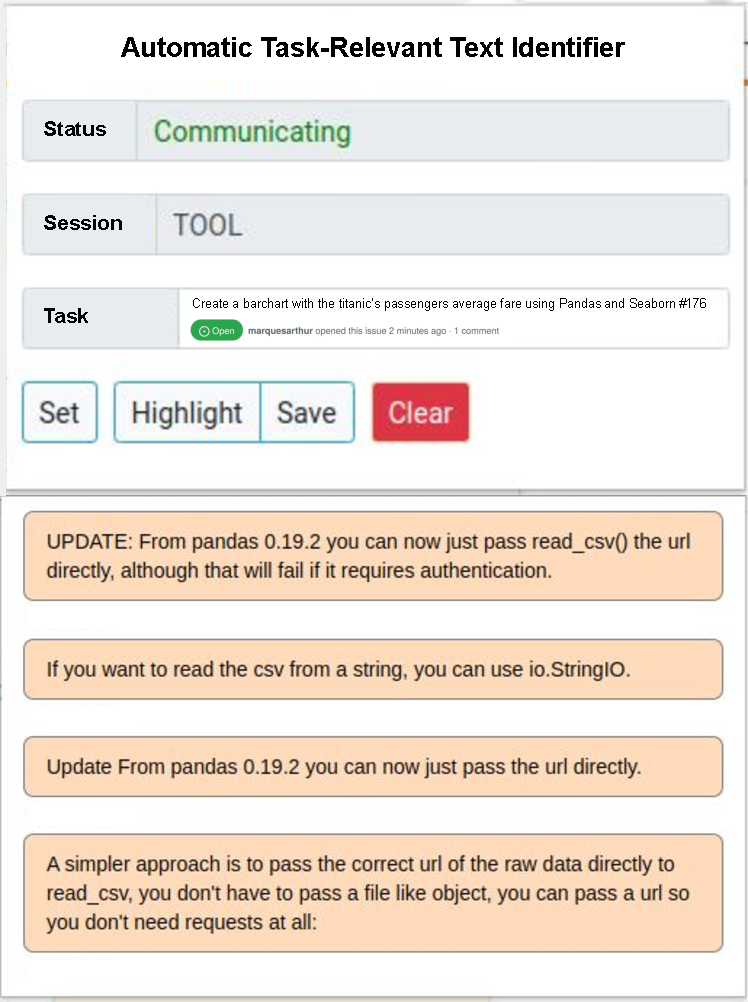
\includegraphics[width=0.5\textwidth]{fig/cp7/navigational-cues}
    \caption{Mock up of the highlights identified by \acs{tool} as navigational cues; by clicking on a highlight, a user could be directed to the part of a document containing that highlight}
    \label{fig:navigational-cues}
\end{figure}



A second approach to organizing the text identified could consider 
the semantic meaning of each sentence, as extracted through frame semantics or other semantic-based approaches. 
For instance, semantic frames could 
assist a user in comprehending the content of the text automatically identified
without the need to read it. 
Similar to Libra~\cite{Ponzanelli2017}, semantic frames could also be used to group the text identified in bubbles or a hierarchical representation 
 helping a developer
in deciding what portions of the text they would inspect first. 
Figure~\ref{fig:semantic-cues} shows a mock up 
with some of the semantic frames extracted 
for the sentences in Figure~\ref{fig:navigational-cues}.
Using the semantic frames identified,
a developer could decide whether they would read sentences 
describing some coding procedure (\textit{execution}), or sentences 
with warnings or requirements (\textit{requirement} and \textit{being obligated})
about the Pandas API. 
To be useful, future research must consider how to identify 
which frames, from all the frames available in a sentence, 
better summarize the meaning of the text. 







\begin{figure}[H]
    \centering
    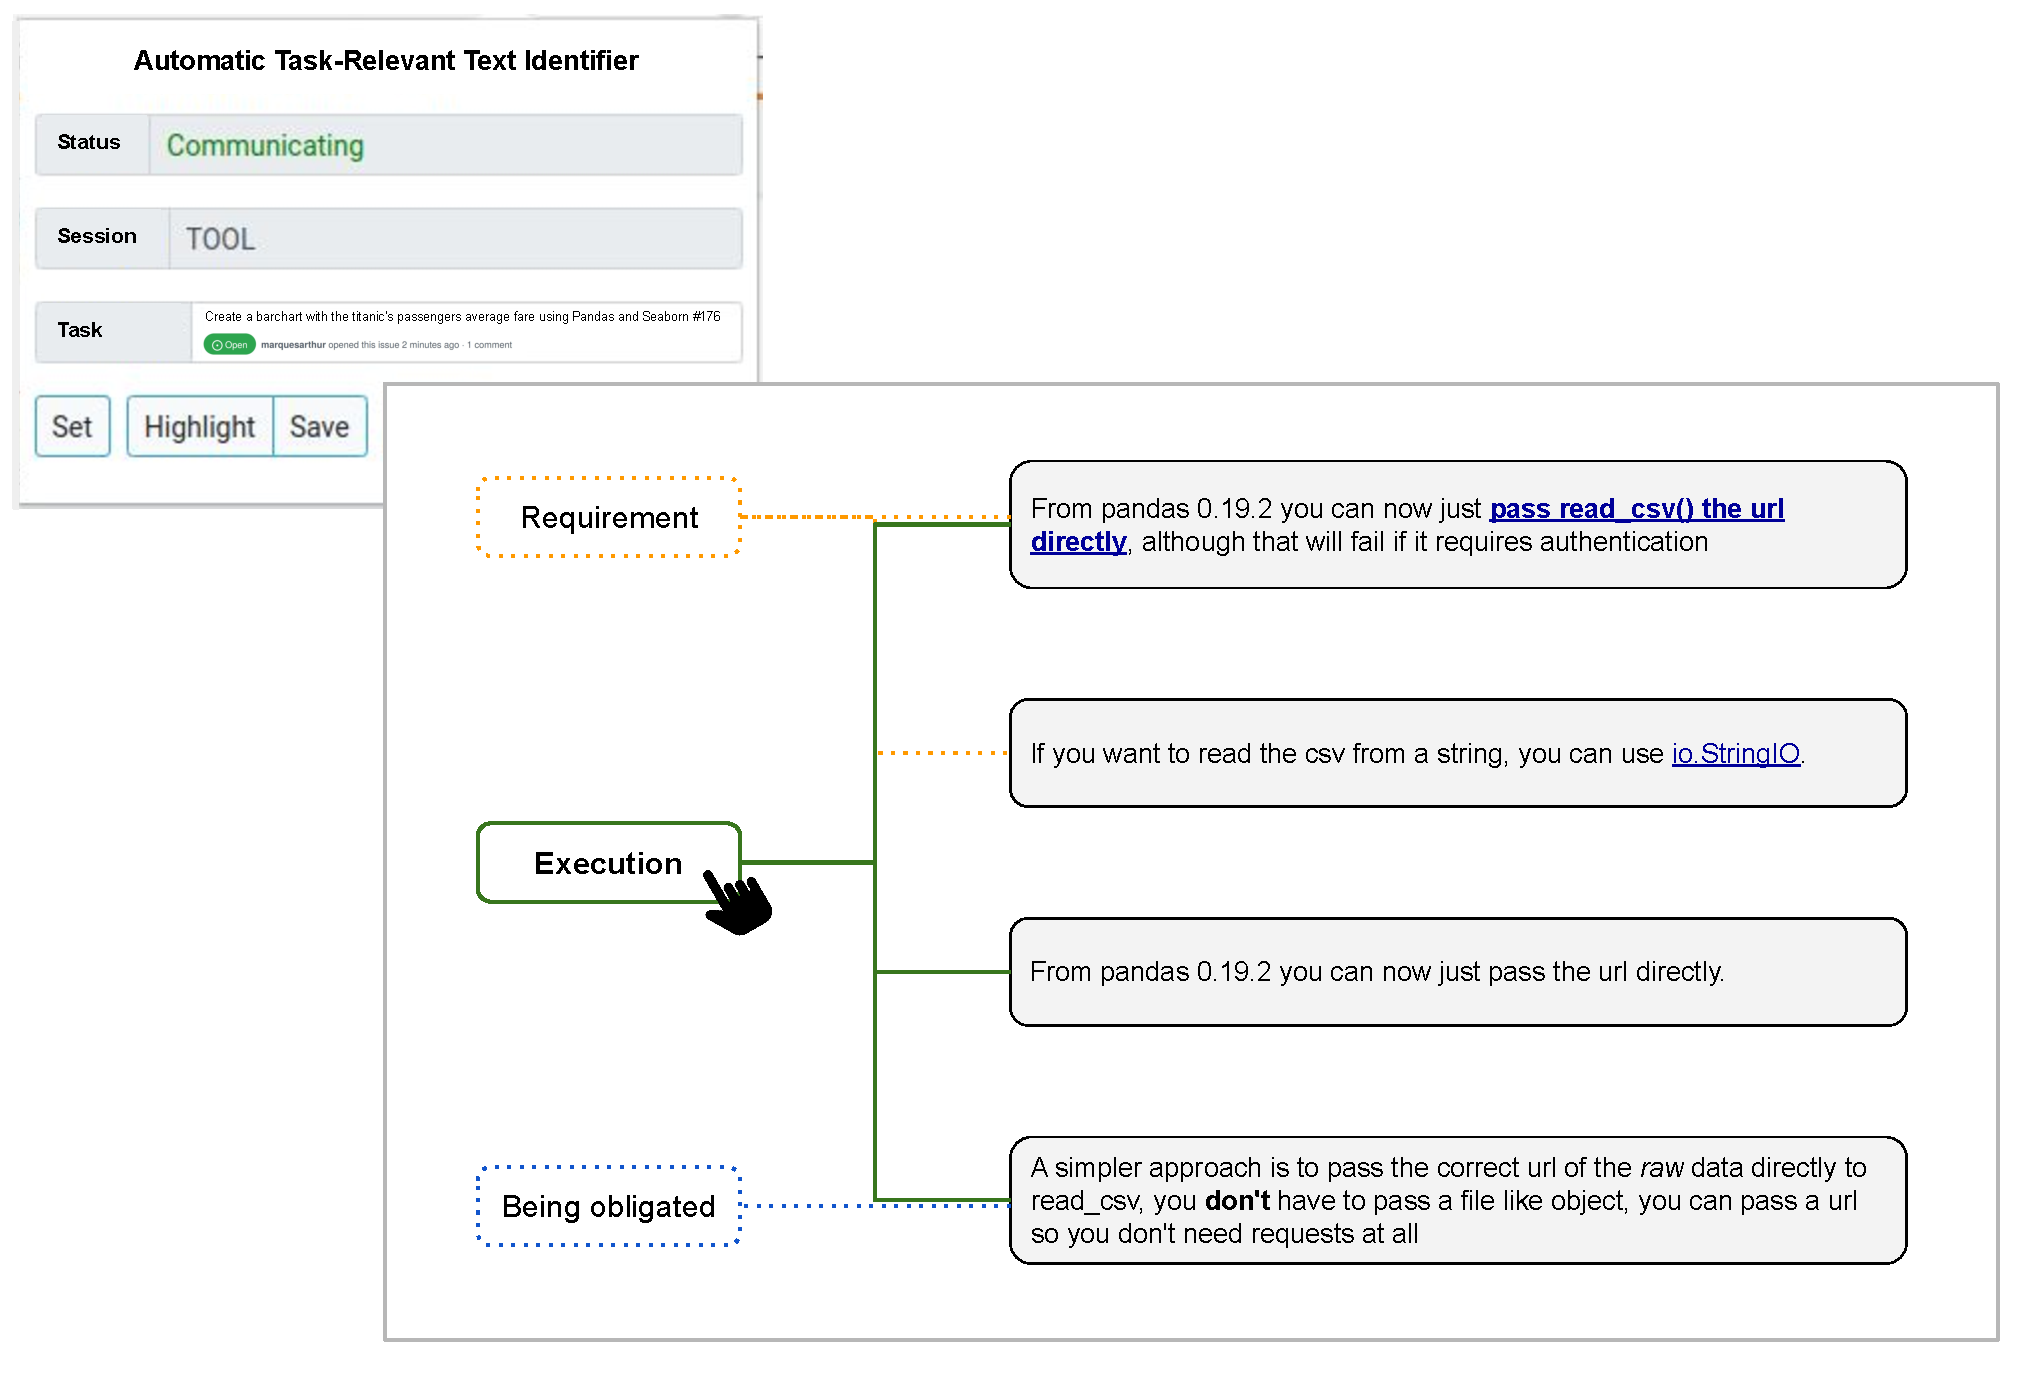
\includegraphics[width=0.95\textwidth]{fig/cp7/semantic-cues}
    \caption{Mock up of the highlights grouped by semantic frames; by hovering over a semantic frame, a user could quickly identify which of the text identified is associated with a certain semantic frame}
    \label{fig:semantic-cues}
\end{figure}






% \setcounter{chapter}{7}


\chapter{Summary}
\label{ch:summary}






\clearpage

\clearpage

%%%%%%%%%%%%%%%%%%%%%%%%%%%%%%%%%%%%%%%%%%%%%%%%%%%%%%%%%%%%%%%%%%%%%%

\begin{singlespace}
\raggedright
\bibliographystyle{abbrvnat}
\bibliography{biblio}
\end{singlespace}

\appendix
%    6. Appendices (including copies of all required UBC Research
%       Ethics Board's Certificates of Approval)
% \chapter{Supporting Materials}

This would be any supporting material not central to the dissertation.
For example:
\begin{itemize}
\item additional details of methodology and/or data;
\item diagrams of specialized equipment developed.;
\item copies of questionnaires and survey instruments.
\end{itemize}


\backmatter
%    7. Index
% See the makeindex package: the following page provides a quick overview
% <http://www.image.ufl.edu/help/latex/latex_indexes.shtml>


\end{document}